%\documentclass{revtex4-1}
\documentclass{book}
\usepackage[T2A]{fontenc}
\usepackage[utf8]{inputenc} % Выбор языка и кодировки
\usepackage[english,russian]{babel}
\usepackage{minted}
%\usepackage{listings}
%\usepackage[cmap]
\usepackage[pdftex]{graphicx}
\usepackage{amsmath}
\usepackage{amssymb}
%%\usepackage{upgreek}
%%\usepackage{siunitx}

\graphicspath{{./figures/}}

\usepackage{hyperref}
\hypersetup{
  colorlinks=true,
  allcolors=blue
}

%\lstset{language=Haskell}

\begin{document}

\title{Программирование для физиков}

\date{\today}
\author{Е. Н. Неруш}
%\email{nerush@appl.sci-nnov.ru}
%\affiliation{ИПФ РАН}
%\affiliation{ННГУ}

%\begin{abstract}
%C$++$
%\end{abstract}

\maketitle

\tableofcontents

\section{Введение}

TODO теория категорий, соответствие Карри--Говарда

В настоящее время почти ни одна статья по физике не обходится без компьютерного моделирования. В
сравнительно простых задачах оно позволяет выявить ошибки в аналитических моделях (хотя бы часть!).
В сложных задачах компьютерное моделирование позволяет <<заглянуть>> в области, недоступные в
настоящее время для эксперимента, например, узнать, что будет происходить с веществом в поле
магнетаров, по напряжённости намного большем доступного в настоящее время в лабораториях лазерного
поля. Часто эксперимент сам по себе настолько сложен, что требует компьютерной обработки
полученных данных (например, LIGO,  Event Horizon Telescope, эксперименты CERN). Однако стоит
помнить, что моделирование всегда основано на уже заложенных в него человеком некоторых базовых
законах, то есть не может существовать в отрыве от теоретических знаний.

Помимо базовых вопросов программирования, численных методов, структур данных и алгоритмов мы будем
здесь касаться вопросов проектирования качественного кода, а также вопросов, связанных с так
называемым <<метапрограммированием>>. Часто можно услышать, что ни то, ни другое не нужно. Однако
из-за того, что компьютерное моделирование прочно вошло в физику, обострилась проблема
воспроизводимости результатов. Код, содержащий ошибки, легко может привести к новым <<открытиям>>,
которые не имеют отношения к физической реальности. Код, написанный плохо, никто не сможет
проверить. Можно ли доверять результатам, полученным с его помощью? Что делать, если у двух разных
научных групп есть две программы для моделирования одной и той же задачи, которые дают разные
результаты? Решением (пусть и частичным) всех этих проблем видится публикация кода (как правило,
под открытой лицензией MIT или BSD) вместе со статьями, описывающими полученные результаты.

Метапрограммирование (в частности, использование шаблонов в C++) позволяет повысить качество кода и
возможности его проверки, уменьшить количество ошибок. Но, возможно, важнее даже то, как
метапрограммирование перестраивает мышление человека. Прежде всего, оно учит абстрактному мышлению,
учит отбрасывать всё лишнее, что само по себе является немаловажным умением не только для
программиста, но и для физика.

Несмотря на большие возможности компьютерного моделирования, стоит помнить, что оно ни в коем
случае не может заменить науку полностью. Цель науки --- не просто научиться воспроизводить
результаты эксперимента, цель - построение картины окружающего мира, который, что само по себе
удивительно, --- познаваем. Мы всегда можем выделить основные эффекты в любом, даже сложном,
явлении, можем <<уложить их в голову>> или описать <<на пальцах>>, и построить простые
аналитические модели, обладающие предсказательной силой. И это прекрасно.

Здесь я хотел бы привести пару ссылок. Во-первых,  \href{https://github.com/EvgenyNerush}{в моём
профиле на Github} можно найти примеры научного кода. Во-вторых,
\href{https://habr.com/ru/users/271828/posts/}{в моём профиле на Хабре} можно найти статьи,
перекликающиеся с темами этих лекций.

\section{Историческая справка}

Сегодня компьютеры используют, например, для проектирования зданий (с 70-x 80-x годов), управления самолётами и
автомобилями, для игры в шахматы и т. д. Как решали раньше задачи, которые требуют огромного
количества вычислений сегодня? Предположим, что нам нужно построить кирпичную арку. Сегодня мы
можем нарисовать что угодно на компьютере и смоделировать напряжения материала. Соответственно, мы
можем подобрать форму так, чтобы напряжения были минамальны и арка не разрушилась бы. Другой способ
--- построить теорию арки, вычислить её форму аналитически. Третий способ --- физическое
моделирование (аналоговые вычисления). Можно заметить, что на каждый кусочек веревки, подвешенной
за два конца, силы действуют только по касательной. Этого же мы хотим добиться, если складываем
арку из кирпича. Таким образом, можно использовать форму веревки для конструирования арки.

\begin{figure}
	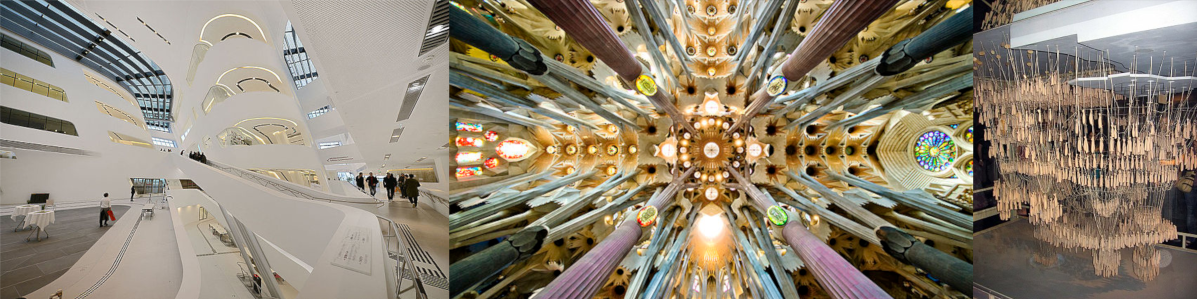
\includegraphics[width=1\linewidth]{arches.png}
    \caption{Слева направо: Венский Университет Экономики и Бизнеса (библиотека и учебный центр,
    2013, Заха Хадид, фотография Böhringer Friedrich), свод храма Святого Семейства, Барселона
    (1882, Антонио Гауди) и одна из веревочных моделей Гауди.}
\end{figure}
\begin{figure}
	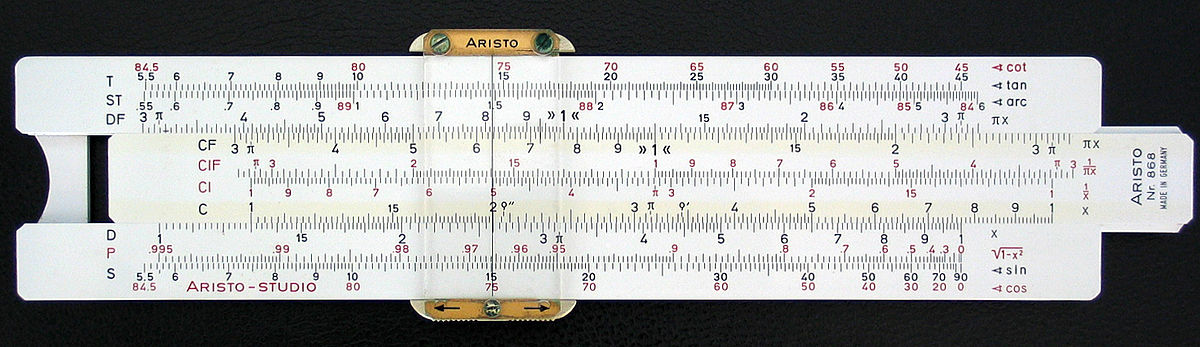
\includegraphics[width=1\linewidth]{sliderule.png}
    \caption{Логарифмическая линейка. Показано умножение чисел $1.3$ (шкала D) на $2$ (шкала C),
    ответ --- на шкале D, $2.6$.}
\end{figure}

Родилась вычислительная техника из общей проблемы проведения сложных вычислений.
Сначала использовали таблицы (с вычисленными вручную значениями) и аппроксимацию, позже, в XVII
веке, изобрели логарифмическую линейку. Идея:
\begin{eqnarray}
    \log(xy) = \log x + \log y,\\
    \log(x / y) = \log(x) - \log(y).
\end{eqnarray}

Арифмометры --- механические вычислительные машины для точного сложения и других операций появились
приблизительно в то же время. Первой ласточкой была машина Паскаля (19 летний Блез хотел помочь
своему отцу, сборщику налогов, с его расчётами; 1642 год), в 1673 году Лейбниц, мотивированный
астрономическими вычислениями, создал свой арифмометр. С тех пор арифмометры широко
распространились и выпускались до 70-х 80-х годов двадцатого века.

Более универсальной, по сравнению с простыми арифмометрами, была разностная машина Чарльза Бэббиджа
(начало XIX века), предназначенная для для вычисления многочленов и разностной аппроксимации,
которая, как и большинство арифмометров, использовала десятичную систему счисления. В
ходе работы у Бэббиджа возникла идея создания универсальной вычислительной машины, которую он
назвал аналитической и которая стала прообразом современного цифрового компьютера. В единую
логическую схему Бэббидж увязал арифметическое устройство, регистры
памяти, и устройство ввода-вывода, реализованное с помощью
перфокарт трёх типов. Перфокарты операций переключали машину между режимами сложения, вычитания,
деления и умножения. Перфокарты переменных управляли передачей данных из памяти в арифметическое
устройство и обратно. Числовые перфокарты могли быть использованы как для ввода данных в машину,
так и для сохранения результатов вычислений, если памяти было недостаточно. Ни разностная, ни
аналитическая машины не были построены, однако первая компьютерная программа была написана именно
для разностной машины Бэббиджа (вычисление чисел Бернулли, 1843 год, Ада Лавлейс). Программа, по
сути, была написана на ассемблере --- она описывала, какимы входными значениями должны быть
заполнены "регистры", какие операции (низкоуровневые --- умножение, сложение, деление) и между
какими регистрами нужно производить. В программе были циклы и в целом она содержала 25 строк, но
работа Ады над ней заняла около года --- на самом деле программа довольно непростая.

qwe
Двоичная система - проще делать устройства. Задачки на перевод. Шестнадцатеричная система.

Конрад Цузе: Z1 (механическая программируемая, 1938 г.), Z3 (на реле, также
программируемая, вычисление корня) --- для чисел с плавающей запятой
(использовалось двоичное представление, не было условных переходов и циклов) ---
май 1941 г., Германия. Расчёты для управляемых ракет, аэродинамика. Z4,
Планкалкюль (подпрограммы, циклы, массивы).

Задача. Логика на реле. Вычисление суммы на реле.

ENIAC, 1943, таблицы стрельбы. Реле (нарисовать устройство), электронные лампы.

Энигма --- портативная шифровальная (и дешифровальная) машина, с начала 1930-х
годов. Шифр замены, провода, диски и лампочки с буквами.

Лоренц, шифр Вернама. Ключ XOR текст даст шифротекст, который может быть
расшифрован при знании ключа. Взлом в 1942 г. из за грубой ошибки оператора.

M-100 Спектр. Довольно большая машина, 140 кг. Суммирование с псевдослучайными
числами на конечном поле. По-видимому, не была взломана.

Turing Bombe, Великобритания, 1940 г. Одна машина эмулировала одновременно
несколько десятков Энигм, перебор ключа при известной открытой части, и Энигма
не шифровала букву саму в себя. Блетчли--Парк, 210 машин, 3 тысячи сообщений
ежедневно.

Проблема разрешения (Гильберт): найти алгоритм, который бы выдавал для
некоторого формального языка и утверждения на нём, истинно или ложно это
утверждение. 1936 г., независимо Алонзо Чёрч и Алан Тьюринг показали
неразрешимость данной проблемы для арифметики, и, следовательно, более общая
проблема неразрешима. Тьюринг для доказательства ввёл понятие машины (Тьюринга). 

Машина Тьюринга способна имитировать любой исполнитель, каким-либо образом
реализующий процесс пошагового вычисления. В её состав входит неограниченная в
обе стороны лента, разделённая на ячейки, и управляющее устройство, способное
находиться в конечном числе состояний. В ячейки на ленте записаны символы
конечного алфавита, либо пустые, либо терминальные (конец работы) символы.
Управляющее устройство работает по правилам перехода, предписывающим в
зависимости от символа в текущей клетке записать в неё новый символ, перейти в
другое состояние или перейти по ленте вправо или влево. Программировать для
такой машины очень сложно.

Вычислимая функция --- функция, которая может быть реализована на машине
Тьюринга. Например, XOR на поле 0, 1. Пусть головка изначально в состоянии 0 и
находится над первым числом, и прописаны следующие правила. 0: 1 - w1r, 0 - w0r.
1: 0 - w1r, 1 - w0r. Машина будет вычислять xor всей последовательности чисел, и
записывать результат, пока не дойдёт до терминального символа. Пример
невычислимой функции --- проблема Гильберта. Проблема останова --- невычислимая функция.

Другой пример вычислимой функции
--- функция Аккермана:
\begin{eqnarray}
    A(m, n) = n + 1, \; m = 0,\\
    A(m - 1, 1), \; m > 0, \; n = 0,\\
    A(m - 1, A(m, n - 1)), \; m > 0, \; n > 0.
\end{eqnarray}
\begin{equation}
    A(1,1) = A(0, A(1,0)) = A(0, A(0,1)) = A(0, 2) = 2 + 1 = 3.
\end{equation}
$A(1,1) = 3$, $A(2,1) = 5$, $A(2,3) = 9$, $A(4,4) = ...$.

Почему можно вычислить за конечное время? Либо $n$, уменьшается, либо $m$.
Рано или позджно $m$ достигнет нуля, однако вычислить реально такую
функцию очень сложно.

Полнота по Тьюрингу. Исполнитель называется тьюринг-полным, если на нём можно
реализовать любую вычислимую функцию. Большинство современных языков
программирования --- Тьюринг-полные. Как доказать --- реализацией машины
Тьюринга на языке.

Теорема о структурном программировании (теорема Бёма -- Якопини, 1965): любая
программа может быть представлена в виде блок схемы с тремя управляющими
структурами: последовательностью, ветвлением и циклом. P\" --- первый полный
по Тьюрингу язык программирования без оператора goto.

FORTRAN, Formula translator, 1954 (первый компилятор)--1957 (оптимизирующий компилятор), IBM.
Первый язык высокого уровня с практическим применением. Начальная цель --- существенно сократить
число строк кода в программе (по сравнению с ассемблером).

Что такое компиляция? Компилятор анализирует ВЕСЬ текст программы, и преобразует его в машинный
код (в низкоуровневый язык, промежуточное представление и т. п. --- что-то положить в такой-то
регистр и т. п.). В простейшем случае работает,
заменяя (транслируя) высокоуровневые функции языка в низкоуровневый код. Например, вместо
\mintinline{cpp}{sqrt(x)}
подставляет конкретный алгоритм вычисления корня. Или (в фортране
появились) --- комплексные числа. На самом деле корень и т. п. вычисляются на floating point unit
(модуль операций с плавающей запятой) внутри процессора --- в нём алгоритмы уже зашиты аппаратно.

Оптимизирующая компиляция.
\begin{minted}{cpp}
    // пусть t на этапе компиляции неизвестно
    x = 0.5 * pi;
    y = pi * pi / 4 - pow((x - pi), 2) + t; // -> t
    x = sin(x + y) + sin(x - y); // -> 2 * cos(t) * sin(x) -> 2 * cos(t)
    // => вдвое меньше нужно вычислять тригонометрических функций!
\end{minted}
На самом деле такая оптимизация возможна только при ffast-math.

Типы данных. Компилятор может производить их анализ (если язык со строгой типизацией) и выдавать
ошибку в случае нарушений:
\begin{minted}{haskell}
    (1 :: Int) / (2 :: Int) -- Error - *div* should be used
\end{minted}

ALGOL (1958 - 1960). Получил распространение как практический язык (в Европе), и как академический
--- для публикации алгоритмов. Программа могла состоять из блоков --- отдельных частей. Ветвления,
циклы, последовательности блоков. Впервые (из промышленных языков) появилась возможность создания
рекурсивных процедур.

На каких машинах это работало? СССР - Большая электронно-счётная машина 6 (1968 --- пошла в серию,
1 млн. операций в секунду, как у американских конкурентов). Были свои трансляторы Фортрана и
Алгола.

LISP. List processing --- обработка списков. Джон Маккарти. Первый интерпретатор - 1958 г. Основан
на идее списков (S-expressions) и ссылках (указателях). Очень простой для синтаксического разбора.
Система автоматического управления памятью, сборщик мусора. Мотивация --- задачи искуственного
интеллекта (шахматы, например).

C. Деннис Ритчи, Bell Labs (aka AT\&T), 1969 -- 1973. Компилируемый статически типизированный язык.

C++, Бьёрн Страуструп, Bell Labs. Начало 80-х. Изначально --- усовершенствования Си для
моделирования телефонный вызовов (теория очередей). Язык стандартизирован, стандарты теперь ---
каждые 3 года. Очень сильное развитие по сравнению с ранними версиями.
1998 — C++ ISO standart. C++11, C++14, C++17, ...

Почему C++? Язык общего назначения, высокая эффективность, широко распространён (много
библиотек), гибкий механизм для конструирования пользовательских типов данных и абстракций,
возможность использовать разные парадигмы программирования, компилируемый, статические типы
данных.
Высокопроизводительные научные вычисления. Сейчас выбор языка уже не так очевиден, хотя
по производительности (предельной) конкуренты только догоняют.

Современное компьютерное моделирование. Что такое наука? Научное знание умещается у человека в
голове. Гипотеза, теория, экспериментальное опровержение. Проблема масштабов и размерностей ---
проблема многих электронов, атомные ядра, многомасштабность в GRBs.

    Задачки на двоичную систему. $2_{10}$, $100_2$. $63_{10}$, $10111_2$. 16-ричная система.
    $64_{10}$, $\mathrm{0xfff}$.

\subsection{Введение в C++}

Типы данных. Статические типы, проверка на этапе компиляции позволяет избежать множества ошибок.
Перегрузка функций.
bool, char, int (2 байта, т.е. 15 бит на значение и 1 бит на знак, $2^{15} - 1 = 32767$),
float, double (8 байт, IEEE 754, binary64, bit for sign, 11 bits for exponent and 53 bits for
fraction,
\begin{equation}
    (-1)^s \left(1 + \sum_{i = 1}^{52} b_{52 - i} 2^{-i} \right) \times 2^{e - 1023},
\end{equation}
 $3 = (2 \times 1.5)$). sizeof()

\begin{minted}{cpp}
#include <iostream> 

using namespace std;

int main( ) { 
    cout << "Hello, world!\n"; 
    return 0; 
    }
\end{minted}

Имена переменных. Инициализация. Оператор присваивания. Арифметика.
\mintinline{cpp}{\%, ==, !=, ++x, +=, \%=}.
\begin{minted}{cpp}
    int k = 18;
    double pi = 3.14159;
    char c = ...;
    z = sqrt(pi); // error - типа нет
\end{minted}

\subsection{Время жизни, область видимости, стэк, куча.}

В задаче о разложении числа (огромного!) и в других задачах у нас возникали последовательности
(множества) чисел. Где их хранить? Оперативная память. Стек и
куча (stack and heap). Стек (стопка), Тьюринг, 1946 г. список элементов, организованных по принципу LIFO
(англ. last in — first out, «последним пришёл — первым вышел»). Пример: вычисления в обратной
польской записи. Указатели. Локальные переменные
процедур размещаются в стеке, при вызове процедур процессор помещает в стек адрес команды,
следующей за командой вызова подпрограммы. Куча. Фрагментация. Управление памятью в куче гораздо сложнее.

\begin{minted}{cpp}
    // simple stack arrays
    int a[5]; // const int, const size_t, etc.
    a[0] = 42;
    std::cout << a[0] << "\t" << a[1] << "\n";
    // g++ warning: a[1] is used uninitialized
    int b[]{1,2,3};
    std::cout << b[0] * b[1] * b[2] << "\n";

    // see also std::array

    // heap arrays, динамические массивы;
    void* p; // указатель на объект неизвестного типа,
             // бывает полезно при преобразовании типов
    int* pi = new int; // int *pi = new int;
    *pi = 3;
    void* pv = pi; // ok
    // cout << *pv << endl; // error
    // могут быть очень большими, много больше стека!
    int main (){
        int n = 10;
        double* d = new double[n];
        d[0] = 3.14;
        cout << d[0] << endl;
        delete[] d;
        return 0;
    }

    // 2d array
    int nx, ny; // потенциальная ошибка...
    nx = 30003;
    ny = 25001; // уже не ограничены стеком
    double** a = new double*[nx]; // ...должны были использовать size_t
    for (int i=0; i < nx; ++i) {
        a[i] = new double[ny];
    }
    a[nx-1][ny-1] = 2.7;
    cout << a[nx-1][ny-1] << "\n";
    for (int i=0; i<nx; ++i) {
        delete[] a[i];
    }
    delete[] a;
    return 0;
    // другой способ --- использовать одномерный массив,
    // с ним порядок прохождения циклов будет не важен
\end{minted}

Передача аргумента по указателю и ссылке. Область видимости, время жизни.
Ссылки. Конструкторы деструкторы, пример! \mintinline{cpp}{& a} читается "ссылка на a".
\begin{minted}{cpp}
    ...
    void f(int x) {
        ++x; 
    }

    void g(int& x) {
        ++x; 
    }
    ... 
    int main() {
        int y = 5; 
        cout << y << "\n"; // 5 
        f(y); 
        cout << y << "\n"; // 5 
        g(y); 
        cout << a << "\n"; // 6
        return 0;
    }
\end{minted}
Передача по указателю...

{\it Задача}. Попробуйт ответить на следующие вопросы. Что такое область видимости
(scope) и время жизни (lifetime) переменной? Где (в стеке или в куче) хранятся переменные
\mintinline{cpp}{a, b, c, d} программы ниже? Где хранится код функции \mintinline{cpp}{f}? Где
потенциальная ошибка в приведённой программе, и что она выведет на экран?

\inputminted{cpp}{lifetime.cpp}

Из приведённого примера становится ясно, что хранение локальных переменных с использованием стека и
время жизни, ограниченное блоками, окружёнными фигурными скобками, прекрасно сочетаются. Так,
создать <<пропуск>> в стеке практически невозможно, то есть невозможно создать ситуацию, при
которой переменная, область видимости которой закончилась, будет <<закрыта>> в стеке переменной
<<сверху>> и не сможет быть удалена из стека. На самом деле, такой ситуации можно бы было добиться
с использованием ключевого слова \mintinline{cpp}{static}, которое позволяет создавать переменные с
временем жизни, большим области видимости (такие переменные инициализируются при первом выполнении
строки с их объявлением, и живут до конца работы программы). Также <<дыры>> в стэке можно было бы
добиться с помощью передачи переменной по ссылке в многопоточной программе, однако, как мы увидим,
в стандартной реализации (C++11) передача аргументов в функцию, исполняемую другим потоком,
возможна только через копирование.


\subsection{Euclid}

(Задача о том, что $p^2 - 1$ делится на 24).

Числа  --- это интересно. Они простые, но образуют очень разнообразные узоры. Например, группы с
умножением по модулю, или простые числа. Сколько простых чисел, меньших заденного целого числа?
Группы Галуа, вязвны с геометрией.

НОД (наибольший общий делитель) двух чисел --- наибольшее число, на которое оба делятся. Как
искать? Перебором?
Строго следовать определению? Составить
таблицу делителей для каждого числа, выбрать совпадающие и найти из них максимальный. Было бы очень
громоздко!

Чем плоха
таблица? Ограниченность, трудно проверить (нужно проверять все числа, а не доказывать алгоритм,
который будет работать для всех. Другой способ --- воспользоваться свойствами функции НОД$(x, y)$ (инвариантность).
Алгоритм
Евклида (Дейкстра, стр. 18). Машина для вычисления НОД$(X, Y)$: лист картона с начерченными линиями
$x = const$, $y = const$, $x + y =
const$ и $x = y$. Если фишка не находится на линии ответа ($x = y$), рассматриваем наименьший
равнобедренный прямоугольный треугольник, у которого вершина прямого угла совпадает с фишкой, а
конец гипотенузы (либо слева, либо снизу фишки) находится на одной из осей. Фишка перемещается в
другой конец гипотенузы, и всё повторяется сначала. Как доказать? Новая точка $x' = x$, $y' = y -
x$, либо $x' = x - y$, $y' = y$. Можно доказать, что НОД$(x, y) = $НОД$(x', y')$, т. е. НОД ---
инвариант нашего преобразования ($x - y$ делится на НОД, числа совпали --- сами себе НОД, и НОД не
может быть больше их, поскольку они на него делятся). Очевидно, конечное число шагов перенесёт
фишку на линию ответа.

Нашем программу, запрашивающую два натуральных числа и выдающую их НОД. Программа
должна использовать оба варианта --- с рекурсией и без, не должна
использовать операцию остатка от деления, а должна использовать алгоритм Евклида, должна
производить сопутствующие проверки (отрицательность, равенство нулю).

Рекурсия на машине Тьюринга (в ф-ии Аккермана, например). К задаче --- Бом--Якопини не требуют
рекурсии.

Напишем программу с рекурсией.
Top-down метод. Легче сначала написать программу с функцией-заглушкой, потом написать простую
функцию через рекурсию, потом без рекурсии, потом добавить проверки...

Первая версия --- Hello, world.
\begin{minted}{cpp}
// euler.cpp
#include <iostream>
using namespace std;

int main() {
    cout << "Hello, world!\n";
    return 0;
}
\end{minted}

Пытаемся скомпилировать и запустить. Добавляем чтение переменных:
\begin{minted}{cpp}
    int a, b;
    cout << "Введите первое число:\n";
    cin >> a;
    cout << "Введите второе число:\n";
    cin >> b;
    cout << "a + b = " << a + b << "\n"; // minted bug
\end{minted}

Для реализации нам понадобится рекурсивная функция gcd (greatest common divisor).
\begin{minted}{cpp}
int gcd(int x, int y) {
    if (x < 0) { // проверка
        return gcd(-x, y);
    } else if (y < 0) {
        return gcd(x, -y);
    } else if (x > y) {
        return gcd(x - y, y);
    } else if (x < y) {
        return gcd(x, y - x);
    } else {
        return x;
    }
}

int main() {
    int a, b;
    cout << "Введите первое число:\n";
    cin >> a;
    cout << "Введите второе число:\n";
    cin >> b;
    cout << "НОД = " << gcd(a, b) << "\n"; // minted bug
    return 0;
}
\end{minted}

\begin{minted}{bash}
    $ g++ euler.cpp # cl euler.cpp
    $ ./a.out # a.exe
\end{minted}

Для версии без рекурсии понадобятся циклы.
\begin{minted}{cpp}
    for(int i = 0; i < 10; ++i ) { // тело выполняется,
                                   // пока выполнено условие i < 10
          cout << i << ...;
    } // можно без {}, но лучше ставить

    // i++ сначала возвращает, потом прибавляет; i++ наоборот
    // i = ++i++; // неопределенное поведение
    for(int i = 0; i<10; cout << ++i << ...) 
        ; // даст 1...10, i++ даст 0...9

    //  while (statement) { expression }
    //  do { expression } while (statement); // тело выполнится хоть один раз

    // gcd без проверок
    /* while (x != y) {
        while (x > y) {
            x = x - y;
        }
        while (x < y) {
            y = y - x;
        }
    } // not beautiful
    */
    while (true) {
        if (x > y) {
            x = x - y;
        } else if (y > x) {
            y = y - x;
        } else {
            break;
        }
    }
\end{minted}

Сложность алгоритма? Сколько операций нужно?

\textit{Задача, множитель 1, deadline 12 апреля}.
Для любого заданного $r \geq 0$ найти все существенно различные формы представления $r$ в виде:
\begin{equation}
    r = x^2 + y^2, \qquad and \qquad x \geq y \geq 0.
\end{equation}
($25 = 3^2 + 4^2 = 5^2 + 0^2$). Для определённости пусть программа выдаёт список пар $(x,
y)$, упорядоченный по возрастанию $x$. Для $74*74*41*41*25*25$ должно получиться $(55370,51840),(56248,50886),..$.

\subsubsection{Фундаментальная теорема арифметики}

Любое натуральное число, большее единицы, имеет единственное разложение на простые сомножители.

Будем считать доказанным, что такое разложение существует. И предположим, что оно не единственное:
\begin{equation}
    N = p_1 \cdot ... \cdot p_r = q_1 \cdot ... \cdot q_s.
\end{equation}
Тогда существует $p_i$, являющееся делителем $N$, но не являющееся делителем ни одного из $q_1, ...
q_s$. Для примера пусть $s = 2$, и пусть $q_1$ не делится на $p_i$. Покажем, что $q_2$ при этом
делится на $p_i$, что докажет нашу теорему. НОД$(p_i, q_1) = 1$ --- числа не делятся. Применим
алгоритм Евклида задом наперёд: $x''^{...} = $НОД$=1$, в то же время $x''^{...} = np_i + mq_1$ (на
первом шаге это так, далее --- по индукции), где $m, n$ --- целые числа (могут быть $<0$):
\begin{equation}
    np_i + mq_1 = 1.
\end{equation}
Умножим на $q_2$:
\begin{equation}
    np_i + mN = q_2.
\end{equation}
$p_i$ является делителем левой части, следовательно --- она делитель и правой части. Теорема
доказана.

Похожая теорема для полиномов (из Галуа)...

\subsection{Задача из Дейкстры (стр. 187) о наименьшем простом множителе большого числа}

Сколько всего простых чисел? Легко доказать, что их бесконечно много. Доказательство Евклида: пусть
есть список простых чисел $p_1$, $p_2$, ... $p_n$. Рассмотрим число $p_1 p_2 ... p_n + 1$. Оно
не делится ни на одно из $p_i$, следовательно оно содержит множителем новое простое число (либо само по себе
простое). Примеры: $2 *
3 + 1 = 7$, $2 * 3 * 5 + 1 = 31$, $2*3*...*11 + 1 = 2311$, простые; составные: $2 * 3 * 5 *
7 * 11 * 13 + 1 = 30031 = 59 * 509$.

Логично исследовать простые числа в качестве возможных множителей в порядке их возрастания.
Максимальный простой множитель не превосходит корня квадратного из этого числа. Если мы не найдем
множителя вплоть до этого корня, это будет значить, что наше число --- простое. Тогда код программы
мог бы быть таким:
\begin{minted}{cpp}
    long long f = 2;
    while (N % f != 0 && f * f < N) {
        f = next_prime(); // how to do this?
    }
    if (N % f != 0) {
        return N; // N is prime
    } else {
        return f;
    }
\end{minted}
Хранение простых чисел в таблице предполагаем невозможным, поскольку исходное число, $N$, считаем
большим (это потребует хранения $O(N^2 / \log N)$ чисел, трюк с корнем существенно
ослабляет требования по хранению, но все равно будем считать хранение неприемлимым). Число можно
вычислять, проверяя на простоту $f + 1$, $f + 2$ и т. д., но проверка на простоту сводится к
проверке, равно ли число своему минимальному простому множителю! Но наименьший простой множитель
числа $N$ является одновременно наименьшим натуральным числом, на которое делится N. Поэтому можно
уйти от проверки на простоту.

\inputminted{cpp}{prime-factors.cpp}

Можно проверить 2 отдельно и дальше проверять только нечетные и т. д., это несколько ускорит, но
усложнит код. Можно упростить вычисление остатка от деления и т. п., но принципиально сложность
вычислений это не изменит.

Если считать вычисление остатка от деления простой операцией, то для нахождения минимального
простого множителя потребуется не более $\sim \sqrt{N}$ операций, сложность $O(\sqrt{N})$. Казалось
бы --- это немного, но если смотреть на зависимость от числа цифр, то получается экспонента: $N
\sim 10^m$ даст сложность $O(10^{m/2})$. Например, максимальное 256-битное число есть $\approx 1.15
\times 10^{77}$, вычисление минимального простого множителя для него может потребовать $10^{38}$
операций!

Мы легко теперь можем найти разложение числа на простые множители (найдем первый, разделим на него
--- далее повторим процедуру поиска, за $O(\sqrt{N})$).

\section{Lehmer random number generator}

Компьютер --- детерменированное устройство (если нет специальной карты для генерации физического
шума), поэтому не может генерировать случайные последовательности чисел, но может генерировать
псевдослучайные последовательности чисел, то есть такие, которые по своим свойствам в определённом
смысле похожи на действительно случайные последовательности. Для многих приложений (интегрирование
методом Монте-Карло, криптография) этого достаточно.

В качестве примера генерации псевдослучайных чисел рассмотрим алгоритм Лехмера. На первый взгляд он
очень простой: следующее псевдослучайное число получается из предыдущего так:
\begin{equation}
    x_{i + 1} = a x_i \mod p.
\end{equation}
Здесь используется операция << умножение по модулю $p$ >>, результат которой есть остаток от
деления на $p$ результата уможения $a x_i$. Например, $2 \times 2 \mod 3 = 1$.

Какие нужно взять $a$ и $p$, чтобы получить <<хорошее>> распределение псевдослучайных чисел и что
вообще значит <<хорошее>>? Давайте посмотрим, что происходит с последовательностью $1..p-1$ при
умножении на $a$, например, для $p = 4$:
\begin{table}[h]
    \centering
    \begin{tabular}{ c | c | c }
        $x_i$ & $2 x_i$ & $3 x_i$ \\
        1 & 2 & 3 \\
        2 & 0 & 2 \\
        3 & 2 & 1 \\
    \end{tabular}
\end{table}
Средний столбец выглядит ужасно --- наш <<генератор>> при $a = 2$ будет генерировать
последовательность нулей для любого входного числа! При $a = 3$ наш генератор будет всегда выдавать
$2$, если $x_0 = 2$, и последовательность $1,3,1,3...$, если $x_0 = 1$ или $3$.  Попробуем взять $p
= 5$:
\begin{table}[h]
    \centering
    \begin{tabular}{ c | c | c | c }
        $x_i$ & $2 x_i$ & $3 x_i$ & $4 x_i$ \\
        1 & 2 & 3 & 4 \\
        2 & 4 & 1 & 3 \\
        3 & 1 & 4 & 2 \\
        4 & 3 & 2 & 1 \\
    \end{tabular}
\end{table}
Здесь всё в порядке (для $a = 2$ или $a = 3$) --- для любого начального числа мы проходим целиком все возможные значения от
$1$ до $p - 1$. Очевидно, что генерируемая последовательность --- периодическая, и период нашей << случайной >> последовательности не может быть
больше, чем $p-1$. То есть мы в данном примере получили максимально возможный период. Кроме того,
каждое число в последовательности на периоде встретится ровно один раз, таким образом, наш
генератор даёт равномерное распределение << случайных >> чисел.

На таких примерах можно прийти к гипотезе, что в качестве $p$ нужно брать
простые числа. Гипотезы в математике очень важны --- иногда они существуют недоказанными многие
годы, существенно влияя, тем не менее, на развитие науки. Так, великая теорема Ферма оставалась
недоказанной около 300 лет.

Интересным примером гипотезы, которая так и не стала теоремой, является гипотеза Эйлера: для любого
натурального $n > 2$ уравнение
\begin{equation}
    \sum_{i = 1}^{n - 1} a_i^n = a_n^n
\end{equation}
не имеет решения в натуральных числах. Например, $a_1^3 + a_2^3 = a_3^3$. Для $n = 3$ гипотеза
верна, для $n = 5$ была опровергнута в 1966 г. с помощью одного из самых <<мощных>> на тот момент
компьютеров, с помощью достаточно <<хитрого>> перебора. Математическая статья, в которой
опровергалась гипотеза Эйлера, состояла буквально из одного предложения:
\begin{equation}
    27^5 + 84^5 + 110^5 + 133^5 = 144^5.
\end{equation}

Вернёмся к генератору Лехмера. Можно доказать следующую теорему.

{\bf Теорема}. Если $p$ --- простое число, то умножение последовательности чисел $1..(p - 1)$ на
любое число $a \in [1, p - 1]$ эквивалентно перестановке последовательности чисел.

Доказательство --- от противного. Предположим, что два числа совпали, то есть
\begin{equation}
    a c_1 \mod p = a c_2 \mod p,
\end{equation}
тогда $a (c1 - c2) \mod p = 0 $, то есть $a (c1 - c2) = n p$.  Последнее равенство не может быть
выполнено, поскольку $a < p$, $|c_1 - c_2| < p$, а $p$ --- простое. Другими словами, при разложении
произведения $a (c1 - c2)$ на множители мы должны среди множителей получить $p$, но каждое из чисел
$a$, $c_1 - c_2$ меньше $p$.

{\bf Следствие 1}. Множество чисел $1..(p - 1)$ с операцией умножения по модулю $p$, где $p$ --- простое,
образуют группу.

Группа --- это множество с ассоциативной операцией (<<умножением>>), для которой в множестве есть
нейтральный элемент (единица; любой элемент не меняется при умножении на неё) и для каждого
элемента есть обратный. Например, группой является множество чисел $1, 2,.., n - 1$, с операцией
сложения по модулю $n$. Единицей в такой группе является число $0$. Такая группа часто обозначается
$\mathbb Z_n$. В качестве упражнения можно попробовать доказать существование обратных элементов
для всех чисел из группы.

В группе, образованной числами $1..(p-1)$ c операцией умножения по модулю $p$, как мы уже доказали,
умножение на $a$ эквивалентно перестановке. Следовательно, при умножении на $a$ единица окажется на
каком-то новом месте, а значит, элемент, обратный для $a$, стоял на месте единицы, таким образом
для любого $a$ существует обратный.

Попробуем ответить на вопрос: какое взять число $a$, чтобы для данного простого $p$ для любого
$x_0$ получался бы максимальный период? Как уже было отмечено, если мы получим максимальный период
($p-1$), то мы построим генератор случайных чисел, дающий, во-первых, много чисел, и, главное ---
дающий числа, имеющие равномерное распределение --- каждое число даст все другие значения по одному
разу. Мы увидим, что для поиска нужного $a$ нам не обязательно переберать для каждого кандидата все
возможные $x_0$.

{\bf Следствие 2}. Множество чисел $1,\; a,\; a^2, ...$, где под умножением подразумевается
умножение по модулю $p$ (следовательно, это конечное множество --- пока не встретится повтора),
образует группу.

Это множество содержится в множестве всех чисел $1...(p=1)$, то есть оно образует
подгруппу группы из следствия 1. Множество $1,\; a,\; a^2, ...$ по определению конечно, в то же время умножение на $a$ эквивалентно
перестановке нашего множества (может показаться, что умножение на $a$ выведет какой-то из элементов
из нашего множества, но по процедуре построения нашего множества этого не может случиться).
Таким образом, единица будет присутствовать в переставленном
множестве, и $a^{-1}$ в исходном множестве находился на том месте, где появилась единица, то есть
$a^{-1}$ в исходном множестве также есть. Отсюда следует интересный вывод: можно не перебирать все $x_0$ для
каждого $a$, а возводить $a$ в степень до тех пор, пока не получится $1$. Если для этого
пришлось возвести $a$ в степень $p$ (то есть при меньшей степени единица не встретилась), то мы
нашли хорошее $a$. Группа, получающаяся из степеней одного и того же элемента (как в нашем случае),
называется циклической, а этот элемент --- образующим группы.

Как долго потребуется возводить $a$ в степень в случае, если в конечном итоге число элементов в
подгруппе $1, a, a^2...$ окажется меньше, чем $p - 1$?  Теорема Лагранжа отвечает на этот вопрос:
порядок (число элементов) конечной группы $G$, для которой группа $H$ --- подгруппа, делится на
порядок группы $H$. Мы не будем её доказывать; наиболее простое и красивое доказательство этой
теоремы использует понятие смежных классов, и может быть легко найдено в Сети.

Из теоремы Лагранжа следует, что порядок нашей подгруппы $1,\; a,\; a^2, ...$ (число элементов)
является делителем для $p - 1$. Например, для $p = 7$: период последовательности $1$, $2$, $2^2 =
4$ ($2^3 = 1$) равен $3$, что делит $p - 1 = 6$. Для $a = 3$ период равен $6$, то есть максимально
возможный.  Таким образом, для создания <<хорошего>> генератора мы можем выбрать простое и
достаточно большое $p$, и $a$ такое, что его степени дадут полную последовательность $1..(p - 1)$
(для поиска таких чисел на самом деле существуют более эффективные методы, чем рассмотренный здесь
перебор, при котором мы идём, пока не встретим единицу). Тогда при любом $x_i$ (он окажется одной
из степеней $a$) мы получим максимально возможный период, а генератор будет давать равномерно
распределённые псевдослучайные числа.

В C++11 функция \mintinline{cpp}{minstd_rand} использует $p = 2^{31} - 1 = 2\,147\,483\,647$ и $a =
48271$ (оба числа простые). Максимальный делитель $p - 1$ есть $331$, поэтому даже перебор всех
возможных $a$ был бы не очень долгим.

У генератора Лехмера можно обеспечить большой период и равномерность распределения, но мы не
контролируем другие его статистические свойства. Например, параметры
можно выбрать настолько плохо (как в случае известного генератора RANDU), что в трёхмерном пространстве (первое число --- координата
по $x$, второе --- по $y$, третье --- по $z$) точки, сгенерированные таким методом, лягут всего на (около) 15
плоскостей. Также может оказаться, что если смотреть на минорные (младшие) биты сгенерированных
чисел, то окажется, что последовательность, составленная из них, имеет гораздо меньший период, чем
$p - 1$. Например, при совсем неудачном выборе параметров можно получить чередование чётных и нечётных
чисел. Поэтому в настоящее время распространение получили другие генериторы псевдослучайных чисел,
такие
как генераторы семейства xorshift (например, xorshift1024*).

\section{Алгоритм быстрого возведения в степень (exponentiation by squaring) и параметрический
полиморфизм (шаблоны)}

Если следовать определению, то возведение числа в целую положительную степень можно было бы
реализовать примерно так:
\begin{minted}{cpp}
    // n^m
    int n = 5;
    int m = 3;
    int p = 1;
    for (int i = 0; i < m; ++i) {
        p = p * n;
    }
    std::cout << p << '\n'; // 125
\end{minted}
При этом, очевидно, сложность данного алгоритма есть $O(m)$.

Еще в XV веке был предложен гораздо более быстрый алгоритм. Рассмотрим сначала его суть на
простейших примерах. Число $2^5$ может быть представлено как $2 \times 2 \times 2 \times 2 \times
2$ (4 умножения), с другой стороны, можно выделить возведения в квадрат: $2^5 = 2 \times a$, $a = b
\times b$, $b = 2 \times 2$ (3 умножения). Как это можно формализовать? Если степень нечётная --- просто
умножаем ответ на множитель (степень при этом уменьшается на единицу), если чётная --- возводим
множитель в квадрат (степень при этом делится на два!). Итерируем до тех пор,
пока степень не иссякнет. Благодаря делению степени на два (как минимум, на каждой второй итерации
алгоритма), сложность возведения в степень данным методом будет $O(\log m)$. Реализуем этот
алгоритм на C++:
\begin{minted}{cpp}
    // n^m; exponentiation by squaring
    int n = 2;
    int m = 15;
    int p = 1; // for result
    while (m != 0) {
        if (m % 2 == 1) {
            m = m - 1;
            p = p * n; // for instance, 2^15 = 2 * 2^14
        } else {
            n = n * n;
            m = m / 2; // for instance, 2^14 = (2 * 2)^7
            // do nothing with p in this case
        }
    }
    // Example:
    // 2^15 = 2 * 2^14 = 2 * 4^7 = 2 * 4 * 4^6 = 2 * 4 * 16^3
    // = 2 * 4 * 16 * 16^2 = 2 * 4 * 16 * 256 = 32768
    std::cout << p << '\n';
\end{minted}

\subsection{RSA шифрование}

Рональд Ривест, Ади Шамир и Леонард Адлеман, MIT. Изучая группы, на которых построен генератор
Лехмера псевдослучайных чисел, мы получили $a^{p - 1} = 1 \mod p$, если $p$ --- простое число, a $a
\in [1, ..., (p-1)]$. Для произвольного, не простого, числа $n$, верно следующее соотношение:
\begin{equation}
    \label{fermat}
    a^{\varphi(n)} = 1 \mod n,
\end{equation}
где $a$ --- взаимно простое с $n$, $\varphi(n)$ --- функция Эйлера --- число натуральных чисел от $1$ до $n - 1$, являющихся
взаимно простыми с $n$. Если $n$ --- простое, то, очевидно, $\varphi(n) = n - 1$. Доказать
утверждение~\ref{fermat} можно, рассматривавя множество взаимно простых с $n$ чисел от $1$ до $n -
1$. С операцией умножения по модулю $n$ эти числа образуют группу.

Рассмотрим такое $n$, которое разлагается на произведение всего двух простых чисел: $n = pq$. Тогда
не взаимно простыми с $n$ (и меньшими $n$) будут только числа $pi$ и $q j$, с $i = 1, 2, ..., (q -
1)$, $j = 1,..., (p  - 1)$, следовательно,
\begin{equation}
    \varphi(n) = (p q - 1) - (q - 1) - (p - 1) = (p - 1)(q - 1).
\end{equation}
Тогда из~\ref{fermat}:
\begin{equation}
    \label{RSA}
    a^{1 + m (p - 1) (q - 1)} = a \mod pq
\end{equation}

Можно заметить, что для $a$, не являющегося взаимно простым с $n = pq$, соотношение~\ref{RSA} также
верно. Для этого достаточно, чтобы были выполнено условие $a^{1 + m (p - 1) (q - 1)} = a$ при
умножении по модулю $p$ и при умножении по модулю $q$. Так, для умножения по модулю $p$ имеем $a^{1
+ m (p - 1) (q - 1)} = a (a^{p - 1})^{(q - 1)} = a$, т. к. $a$ и $p$ --- взаимно простые и $a^{p -
1} = 1$ (либо тривиальное $a = 0 \mod p$). Аналогично для $q$. 

Соотношение~\ref{RSA}--- ключевое соотношение в алгоритме RSA.
Предположим, что мы нашли пару чисел $e$ и $d$ таких, что
$de = 1 + m (p - 1) (q - 1)$, то есть $de = 1 \mod (p - 1) (q - 1)$. Тогда мы можем произвести
шифрование, возведя в степень $e$, и дешифрование, возведя зашифрованное число в степень $d$!

Как именно это применяется? Предположим, что Алиса где-то взяла (сгенерировала) числа $p$, $q$, $e$
и $d$. Она может сообщить Бобу пару чисел $(e, n = pq)$ (открытый ключ), не сообщая при этом сами
$p$ и $q$. Тогда Боб может зашифровать своё сообщение $a$, возведя его в степень, $a^e \mod n$ (за
$O(\log e)$ операций), и Алиса сможет также легко расшифровать его сообщение, $(a^e)^d = a$. В то
же время, если кто-то перехватит открытый ключ, для расшифровки сообщения ему потребуется разложить
$n$ на множители, что потребует $O(\sqrt{N})$ операций, то есть экспоненциально сложно по
количеству цифр в $n$.

Где взять большие простые числа $p$ и $q$? Казалось бы, если их находить перебором, то потребуется
слишком много времени на проверку, простые ли они. Однако тесты простоты для чисел
специального вида могут быть проведены гораздо быстрее, чем для произвольных чисел. Например, тест
Люка--Лемера позволяет за полиномиальное время от битовой длины числа Мерсенна ($2^l - 1$)
определить, простое оно или нет.

Здесь следует заметить, что условия компьютерной сети отличаются от условий "прямой видимости"
Алисы и Боба. В сети они передают сообщения только через посредников, которые могут попытаться их
обмануть, осуществив, например, так называемую атаку man in the middle. Суть её в следующем. Алиса
передаёт промежуточному узлу открытый ключ. Промежуточный узел дает Бобу другой (!), свой, открытый
ключ. Боб шифрует им сообщение, промежеточный узел расшифровывает его, читает, и зашифровывает
ключом Алисы, после чего посылает его Алисе. Таким образом, злоумышленник --- промежуточный узел
--- читает всю переписку. Для предотвращения такой атаки необходим другой канал связи между Алисой
и Бобом, который либо недоступен злоумышленнику, либо подмена ключа в котором крайне маловероятна.
Например, Алиса может позвонить Бобу и спросить у него тот открытый ключ, который она передала ему
в компьютерной сети. Если ключ, полученный Бобом, именно тот, что передавала Алиса, то атаки man in
the middle не произошло. Если Боб сообщает Алисе ключ голосом, или в виде картинке (по видеосвязи),
то верояность замены его "на лету" можно считать очень низкой. Хотя в принципе атака man in the
middle не может быть исключена полностью здесь. Таким образом, для создания шифрованного канала
связи нужно однократно использовать дополнительный достоверный канал связи.

В ряде случаев нужно не только зашифровать канал связи, но и скрыть сам факт передачи сообщения от
Алисы Бобу. Как это сделать, если на маршруте в компьютерной сети между Алисой и Бобом находится
злоумышленник? Один из вариантов решения проблемы --- луковая маршрутизация (onion routing),
приближенно сводящаяся к слудующему. Из компьютеров добровольцев создаётся <<луковая сеть>>,
компьютеры которой дают свои ключи шифрования Алисе. Алиса определяет некоторый квазислучайный
маршрут через компьютеры луковой сети, для определенности 3--8--2--1--4--7, и далее к Бобу. К
своему зашифрованному сообщению она добавляет номер последнего компьютера в маршруте, 7, и шифрует
это ключом предпоследнего компьютера и т. д. Луковая чешуя. Tor browser. Уязвимости. Важно помнить,
что если есть хоть какой-то дополнительный канал связи (но достоверный), то препятствовать
шифрованию невозможно.

\subsection{Параметрический полиморфизм}

Если мы оформим алгоритм быстрого возведения в степень в виде функции, то сможем его несколько
улучшить, например, явно указав (с помощью типа), что степень --- целое беззнаковое число. Но
наиболее заметное улучшение можно сделать, заметив, что в натуральную степень можно возводить не
только \mintinline{cpp}{int}, но и \mintinline{cpp}{long int}, \mintinline{cpp}{unsigned long int,
float, double}, хотя с числами с плавающей запятой можно несколько потерять точность. Подобные
обобщения (абстракции) очень часто встречаются в математике, где теоремы стараются формулировать
наиболее <<широко>>.

Как обобщение, описанное в конце прошлой части, можно реализовать? Самый простой способ ---
скопировать код нашей функции много раз, и заменить в этих копиях тип аргумента, которой возводится
в стемень, на те типы, которые нам нужны. Такой подход возможен --- C++ допускает существование в
коде функций, имеющих одинаковое имя, но разный тип аргументов (такая возможность называется
перегрузкой функций). Однако подобный подход имеет ряд существенных проблем. Во-первых, нельзя
заранее предусмотреть, какие именно типы нам понадобятся. В частности, при написании библиотеки
(кода, которым в своих программах будут пользоваться другие программисты) вообще неизвестно, какие
типы понадобятся в будущем (а ведь бывают еще и типы, определённые пользователем!), и такой подход
оказывается в принципе невозможным. Во-вторых, такой код было бы очень трудно поддерживать и
сопровождать. Предположим, что в нашей функции обнаружилась ошибка. Для её исправления нам пришлось
бы переписать все варианты нашей функции, полученные через copy-paste, и никто не гарантирует, что
мы смогли бы их все переписать правильно, не внеся новых ошибок.

Для поддержки абстракций в коде (абстракции такого типа называют <<параметрическим полиморфизмом>>)
и решения описанных проблем был придуман мехинизм шаблонов. Упрощенно его работу можно представить
так. Перед компиляцией исходный код пропускается через программу-предпроцессор, которая ищет вызовы
шаблонных функций и определяет, для каких конкретных типов потребуются реализации шаблонов. После
этого программа-предпроцессор копирует код шаблона, подставляя в качестве шаблонного типа типы, для
которых нужны реализации данной функции. После этого получается код, в котором определены все
функции, которые в нём встретятся. Хотя все эти функции имеют одно и то же имя, но за счёт
поддержки перегрузки функций данный код уже может быть отдан компилятору.

Рассмотрим простой пример.  Чтобы возводить в квадрат (и, главное, получать в качестве результата)
разные типы, используем шаблон.
\begin{minted}{cpp}
    #include <iostream>

    // шаблон; вводим абстрактный тип T,
    // а затем используем его
    template <typename T> T squared(T a) {
        return a * a;
    }

    int main() {
        //         здесь T = double
        std::cout << squared<double>(3.14) // получим 9.8596
                  << '\t'
                  //     T = int
                  << squared<int>(2) // результат = 4
                  << '\n'
                  ;
        return 0;
    }
\end{minted}
При использовании шаблонных функций не обязательно указывать тип в треугольных скобках --- он часто
может быть выведен из типа аргументов функции [например, в случае \mintinline{cpp}{squared(3.14)}
очевидно, что \mintinline{cpp}{T = double}]. Однако не стоит этим злоупотреблять (как минимум,
чтобы программу было проще читать и чтобы не запутаться самому).  Например, в Python
параметрический полиморфизм реализован на первый взгляд проще, но при его использовании гораздо
проще совершить ошибку, по сравнению с C++:
\begin{minted}{python}
    # определение полиморфной (по обоим аргументам!) функции div
    def div(a, b):
        return a / b

    print(div(2, 3)) # int или float?
\end{minted}

Вернёмся к возведению в степень, воспользовавшись шаблонами:
\inputminted{cpp}{pow.cpp}
Размер кода почти не изменился, и теперь у нас есть удобная, понятная функция и её можно
использовать для множества типов!

В C++ шаблоны, как уже было сказано, реализуются, по сути, с помощью копирования кода шаблона и
подстановки того типа, для которого в программе будет вызвана шаблонная функция. На самом деле этот
механизм работает не только для типов, но и для значений (так называемые шаблоны с нетиповыми
параметрами).  При этом, как можно заметить, возможна ситуация, когда одного прохода по коду
недостаточно для того, чтобы определить все значения параметров, необходимых для подстановки в
шаблон, но такой случай также предусмотрен в языке и не является проблемой для компилятора:
\inputminted{cpp}{fac-template.cpp}
При использовании оптимизирующего компилятора вычисление факториала в данном примере будут
проведено еще на этапе компиляции, а в машинном коде уже будет содержаться ответ.

{\it Задача}. Написать программу, которая вычисляла бы числа Фибоначчи тремя способама: через
рекурсию, с использованием цикла и на этапе компиляции через шаблоны.


\subsection{Пользовательские типы}

Во многих задачах мы имеем дело с объектами, для которых нет подходящего типа среди стандартных
типов C++, например, в стандартной библиотеке нет матриц и функций из линейной алгебры. Однако C++
позволяет определять пользовательские типы, такие же удобные, как и встроенные типы. Так, есть
возможность самостоятельно определить матрицы, и переопределить для них (например) оператор
умножения.

В простейшем случае новые типы можно определять, используя структуры:
\begin{minted}{cpp}
    #include <iostream>

    struct pair {
        int a;
        int b;
    }; // обратите внимание на точку с запятой

    int main() {
        pair p = {2, 3}; // или {2, 3,};
        p.a = p.a + p.b;
        std::cout << p.a << '\n'; // 5
        return 0;
    }
\end{minted}
Для работы с \mintinline{cpp}{pair} мы можем определить различные функции. Однако сразу стоит
оговориться, что при передаче арнумента в функцию происходит его копирование, и внутри функции мы
работаем с копией. Это значит, прежде всего, что мы можем потерять в производительности кода (если
функция выполняет мало действий, но вызывается много раз) и в потреблении памяти (если передаваемая
структура очень много <<весит>>). Чтобы избежать подобных проблем, используют передачу по ссылке,
при которой копирования не происходит, а изменения происходят с передаваемым объектом:
\begin{minted}{cpp}
    void f(int x) { // передача по значению
        x = x + 1; 
    }

    void g(int& x) { // передача по ссылке
        x = x + 1; 
    }
    // ... 
    int y = 5; 
    f(y); // y по-прежнему равен 5
    g(y); // теперь y = 6
\end{minted}
Если аргумент, передаваемый по ссылке, модифицируется функцией, то его обычно ставят в начало
списка аргументов. Если же он не модифицируется, стоит указать это явно с помощью ключевого слова
\mintinline{cpp}{const} перед его типом. Вместо ссылки (и для тех же целей) можно передавать в
функцию указатель.

Вернёмся к \mintinline{cpp}{pair}.  Наша пара подойдёт, например, для целочисленных коорддинат, или
для времени (часы, минуты), но ни для координаты с плавающей точкой, ни для людей (имя, фамилия),
ни для продуктов в кулинарном рецепте (название, вес) она не годится, хотя во всех этих примерах
также нужны пары. Для обобщения нашей структуры, как легко догадаться, можно воспользоваться
шаблонами:
\begin{minted}{cpp}
    template <typename A, typename B> struct pair {
        A a;
        B b;
    };
    //...
    pair<int, int>           p    = {2, 3};
    pair<std::string, float> kiwi = {"kiwifruit", 0.2}; // разнородная пара
\end{minted}

Шаблоны открывают широкие возможности абстракции, однако ими (как и многим другим) стоит
пользоваться с умом. В частности, не всегда легко понять, какой именно шаблон будет использован в
конкретном месте:
\inputminted{cpp}{oops_templates.cpp}
Почему в этом примере получилось $334$? Для начала ответим на вопрос, какие реализации шаблонов
могут встретяться в нашем коде? Очевидно, это будут: реализация шаблона $3$ для пары из пар целых
чисел (\textit{3-pair-pair}), реализация шаблона $3$ для пары целых чисел (\textit{3-pair-int}),
реализация шаблона $2$ для типа \mintinline{cpp}{pair<int, int>} (\textit{2-pair-int} и реализация
шаблона $2$ для типа \mintinline{cpp}{int} (\textit{2-int}). При вызове \mintinline{cpp}{oops(p)}
вызывается функция \textit{3-pair-pair} (что даёт $100$), которая вызывает две функции:
\textit{3-pair-int} ($+100$) и \mintinline{cpp}{oops<B>(...)}, где \mintinline{cpp}{B} выводится из
типа аргумента функции \textit{3-pair-pair}, то есть \mintinline{cpp}{B = pair<int, int>}. Таким
образом, в этом случае используется шаблон с одним шаблонным параметром, что приводит к вызову
функции \textit{2-pair-int}, а уже она вызывает \textit{3-pair-int} ($+110$)! Каждая из двух
функций \textit{3-pair-int} вызывает функцию \textit{1} и функцию \textit{2-int} ($+22$). Далее,
функции \textit{2-int} вызывают функцию \textit{1} ($+2$). Итого получается, наконец, $334$.
Проследить эту цепочку вызовов довольно легко, добавив в наши функции \mintinline{cpp}{cout}
номеров функций.  Хочется верить, что этот пример не отпугнёт читателя от использования шаблонов, а
научит использовать шаблоны с осторожностью, не смешивая шаблонные и нешаблонные функции, и шаблоны
с разным числом параметров, а заодно не экономить, и писать скобки \mintinline{cpp}{<...>}, там,
где они подразумеваются, не надеясь на автоматический вывод.

Теперь попробуем ответить на вопрос, что будет, если мы вызовем \mintinline{cpp}{oops(r)}? Через ту
же цепочку она приведёт к вызову \mintinline{cpp}{oops<double>(...)} (реализация второго шаблона),
которая рекурсивно вызывает саму себя до бесконечности!

Вернёмся к пользовательским типам, говоря о которых, часто начинают с объектно-ориентированного
подхода, то есть с классов, инкапсуляции и наследования. Здесь мы намеренно откладываем эти темы,
поскольку структур и шаблонов уже достаточно для построения качественного кода, и вполне достаточно
для решения слещующей задачи.

\textit{Задача. Числа Фибоначчи.}
Рассмотрим задачу вычисления чисел Фибоначчи: $F_0 = 0$, $F_1 = 1$, $F_n = F_{n-1} + F_{n-2}$.
Фибоначчи (Леонардо Пизанский, первый крупный математик средневековой Европы, 1170--1250) пришёл к
этой последовательности, как к решению абстрактной задачи о размножении кроликов. Вычислять числа
Фибоначчи можно по-разному. В данном случае требуется написать три функции, вычисляющие число
Фибоначчи для заданного номера $n$ разными способами, и, желательно, измерить время работы функций.
Первый способ --- с использованием простой рекурсии. Второй способ --- с использованием циклов.
Требуется, чтобы вычисление вторым способом было принципиально быстрее, чем первым. Третий способ
связан с тем, что вычисление чисел Фибоначчи можно представить с помощью матриц:
\begin{equation}
    \begin{pmatrix}
        F_n \\
        F_{n-1}
    \end{pmatrix} =
    \begin{pmatrix}
        1 & 1 \\
        1 & 0
    \end{pmatrix}
    \begin{pmatrix}
        F_{n - 1} \\
        F_{n - 2}
    \end{pmatrix} =
    \begin{pmatrix}
        1 & 1 \\
        1 & 0
    \end{pmatrix}^{n - 1}
    \begin{pmatrix}
        1 \\
        0
    \end{pmatrix}.
\end{equation}
Таким образом, задача свелась к возведению матрицы в степень. В данном случае нужно создать
структуры для представления матриц в программе, написать шаблонную функцию для возведения в степень
быстрым алгоритмом (exponentiation by sqyaring), определить оператор умножения для матриц, и
собрать всё это вместе. Для всех трёх способов вычисления необходимо оценить сложность в терминах
$O$-нотации. Программа должна при запуске выводить на экран $F_{9}$, $F_{34}$ и $F_{50}$
(получающиеся значения стоит указать, например, в комментариях в коде).
% $F_{9} = 34$, $F_{34} = 5702887$, $F_{50} = 12586269025$, в последнем случае необходимо для
% возыращаемого значения использовать long long int.

\clearpage

Например, можно написать функцию, поэлементно перемножающую два массива:
%\inputminted{cpp}{mult-arrays.cpp}
(не так!!! qwe) При этом, что очень важно, мы избавляемся от ряда возможных ошибок: например, если мы вызовем нашу
функцию для массивов разной длины, код просто не скомпилируется.

\subsection{Задача --- числа Фибоначчи}
Рассмотрим задачу вычисления чисел Фибоначчи. $F_0 = 0$, $F_1 = 1$, $F_n = F_{n-1} + F_{n-2}$.
$F_{12} = ?$.
13 век, задача о кроликах. Эти
соотношения можно представить в виде матрицы:
\begin{equation}
    \begin{pmatrix} F_n \\ F_{n-1} \end{pmatrix} = \begin{pmatrix} 1 & 1 \\ 1 & 0 \end{pmatrix}
    \begin{pmatrix} F_{n - 1} \\ F_{n - 2} \end{pmatrix} = \begin{pmatrix} 1 & 1 \\ 1 & 0
\end{pmatrix}^{n - 1} \begin{pmatrix} 1 \\ 0 \end{pmatrix}.
\end{equation}
Задача --- написать функцию-шаблон для возведения в степень быстрым алгоритмом, вычислить с помощью
неё числа Фибоначчи. Сравнить с рекурсивным и линейным алгоритмами. (Тип
\mintinline{cpp}{long long int} имеет длину не менее 64 бит, \mintinline{cpp}{long int} --- не
менее 32). Вычислите $F_{45} < 2^{31}$, $2^{31} < F_{47} = 2971215073 < 2^{32}$, $F_{50} =
12586269025 > 2^{32}$.  Какой тип возвращаемого значения должна иметь функция для вычисления
каждого из этих чисел?  (Проверка: $F_{9} = 34$, $F_{34} = 5702887$). Ниписать тремя способами.

\clearpage
\textit{Задача}. Дано множество чисел $\{0,1,2,3,4\}$ с операцией сложения по модулю $5$. Докажите,
что данное множество образует группу. Найдите все её подгруппы.

\section{Математический маятник. Метод Эйлера и метод средней точки.}

Задача об осцилляторе.

wolframalpha.com: dx/dt=v, dv/dt=-x, x(0) = 0, v(0) = 1

Решение: $x = sin(t), \; v = cos(t)$.

Метод Эйлера: $x_{n+1} = x_n + v_n \Delta t$, $v_{n+1} = v_n - x_n \Delta t$, на Cpp:

\begin{minted}{cpp}
#include <iostream> 
using namespace std;

int main( ) { 
    double x, v, t, dt; // or float
    x = 0; 
    v = 1; 
    t = 10; 
    dt = 0.1; 
    int i; // or long int (long)
    for(int i=0; i < int (t / dt); ++i) { 
        float a = x; 
        x = x + v * dt; 
        v = v - a * dt; 
        cout << x << "\t" << v << "\n";
    } 
    cout << "Bye!\n";
    return 0; 
}
\end{minted}
За $t = 10$ (а чему равен период маятника?) амплитуда доросла до $1.5$! На самом деле она растёт
экспоненциально. При $dt = 0.01$ амплитуда доходит до $1.05$, но поскольку она растёт
экспоненциально, практически никакое уменьшение шага не спасёт на больших временах: при $t = 100$
получаем те же самые $1.5$. Почему так происходит?

Задачи для решения у доски. Написать аналитическое решение для численной схемы Эйлера (ещё один вид
маятника). Решение: $(x_n, v_n) = (x_0, v_0) \cdot e^{i \omega n \Delta t}$, что даст
\begin{equation}
    (1 - e^{i \omega \Delta t})^2 = -\Delta t^2.
\end{equation}
Дальше можно найти $\omega$ в виде $\omega = \omega_0 + \omega_1 ...$, где $\omega_0 = O(1)$ и
$\omega_1 = O(\Delta t^2)$ (получится, что
$\omega_0 = 1$, а $\omega_1 = -i \Delta t / 2$? --- имеет отрицательную мнимую часть, что в решении
даст нарастающую экспоненту).

Таким образом, проблема не просто в точности решения!

\subsubsection{Midpoint}

Давайте попробуем увеличить точность метода Эйлера и посмотрим, что из этого получится. Из картинки
$x(t)$ понятно, что точность у метода Эйлера хуже там, где кривизна больше. Интуитивно понятно, что
если взять производную в средней точке ($x_{n+1}$ определять через $v_{n + 1/2}$), то точность
решения будет выше. Midpoint, Leap frog.
\begin{eqnarray}
    x_{n + 1} = x_n + v_{n + 1/2} \Delta t, \\
    v_{n + 3/2} = v_{n + 1/2} - x_{n + 1} \Delta t.
\end{eqnarray}
(Внимание на индексы). Во-первых, не для любого уравнения так можно сделать, во-вторых, нужно не
забывать на пол-шага сдвигать, например, скорость в начале. Что при этом будет с устойчивостью ---
задание для решения у доски. Должно получиться $(e^{i \omega \Delta t} - 1)^2 = -\Delta t^2 e^{i
\omega \Delta t}$, что даёт
\begin{equation}
    \sin^2 \frac{\omega \Delta t}{2} = \left( \frac{\Delta t}{2} \right)^2.
\end{equation}
Очевидно, что решение ($\omega$) вещественное, то есть неустойчивости нет, пока $\Delta t < 2$.

\subsubsection{Задача (10.03): pi + период физического маятника}
(7 баллов = 1 б. значение pi, 3 б.
период от амплитуды (картинка, правильная) + 1 б. метод средней точки + 1 б. корректно выбраны начальные
условия + 1 б. линейная аппроксимация для уточнения места нуля скорости.)

Написать программу реализующую метод средней точки для уравнений математического маятника, и
физического маятника:
\begin{eqnarray}
    \frac{dx}{dt} = v, \\
    \frac{dv}{dt} = - \sin x.
\end{eqnarray}
Определить период колебаний, и для математического маятника вычислить из него число $\pi$, а для
физического построить зависимость периода от начальной амплитуды. Присылать шаги и полученное
значение пи, версию с физическим маятником и картинку с периодом от амплитуды.

Что с точностью данных схем? Рассмотрим простое уравнение (получим точное решение численных схем у
доски):
\begin{equation}
    \frac{dx}{dt} = t
\end{equation}
Схема Эйлера нам даст:
\begin{equation}
    x_n = x_0 + \Delta t^2 \sum_{i = 1}^n i = \frac{\Delta t^2 N (N + 1)}{2} = \frac{t^2}{2} +
    \frac{t \Delta t}{2}.
\end{equation}
O-нотация.

Схема midpoint:
Получится точное решение, поскольку на одном шаге схема даёт точное решение.
\begin{eqnarray}
    \frac{x_{n+1} - x_n}{\Delta t} = t_{n+1/2} = (n + 1/2) \Delta t, \\
    x_{n + 1} = x_n + (\Delta t )^2 \times (n + 1/2),
\end{eqnarray}
Если предположить, что $x_n = t_n^2 / 2$, то есть найдено точно, то и $x_{n + 1}$ найдено точно:
\begin{equation}
    x_{n + 1} = \frac{\Delta t^2 (n^2 + 2 n + 1)}{2} = \frac{(n + 1) \Delta t}{2}.
\end{equation}
Начальное условие известно точно ($x_0 = 0$), дальше делаем шаги и т. п.
Другой способ, для любого начального условия --- просто суммируем ряд:
\begin{eqnarray}
    x_{n + 1} = x_n + \Delta t^2 \times (n + 1/2) = \\
    x_{n + 1} = x_{n - 1} + (n - 1 /2) \Delta t^2 + (n + 1 / 2) \Delta t^2 = \\
    x_0 + \Delta t^2 \times \left\{ \sum_{i = 0}^n (i + 1/2) \right\} = \\
    x_0 + \Delta t^2 \times \left\{ \frac{n (n + 1)}{2} + (n + 1) / 2 \right\} = \\
    x_0 + (\Delta t)^2 \times \frac{(n + 1)^2}{2}.
\end{eqnarray}
$x(T = t_N = N \Delta t)$, $n + 1 = N$,
\begin{equation}
    x_n = x_0 +(\Delta t)^2 \times \frac{N^2}{2} = x_0 + T^2 / 2.
\end{equation}
Почему получилось точное решение? Высшие производные равны нулю! Ряд Тейлора для Эйлера и средней
точки. Снова O-нотация.

Не для любой правой части можем написать схему средней точки. Рассмотрим другое уравнение:
\begin{equation}
    \frac{dx}{dt} = -x, \qquad x(0) = 1,
\end{equation}
(Если sin x справа, то уже метод средней точки в простом виде не пройдёт).
Должно получиться $x_{n+1} = e^{-(n+1) \Delta t}$.

Эйлер:
\begin{equation}
    x_{n+1} = x_{n} - \Delta t \times x_n = (1 - \Delta t)^{n + 1} x_0.
\end{equation}
Midpoint (leap frog):
\begin{eqnarray}
    x_{n+1} = x_{n} - \frac{\Delta t}{2} \times (x_n + x_{n+1}), \\
    x_{n+1} = \left\{ (1 - \Delta t / 2) / (1 + \Delta t / 2) \right\}^{n+1} x_0.
\end{eqnarray}
Анализ --- чему равна ошибка на первом шаге. Снова ряд Тейлора (разложим аналитическое решение...).

\section{Простые алгоритмы}

Как вычислять, например, обратное число или корень?
Методы нахождения нуля функции. Метод деления пополам. Метод Ньютона.

Multiplicative inverse algorithm.
\begin{eqnarray}
    b = a^{-1} + x, \\
    ax = ab - 1, \\
    b_{i + 1} = b_i - b_i (ab_i - 1).
\end{eqnarray}
Newton-rhapson algorithm.
$a_{i+1} = (a_i + n / a_i) / 2$

Как эти методы выглядят с точки зрения конечно-разностных схем для решения дифф уравнений?

  $f(0) = 1$, $f(n>0) = \sqrt{2 + f(n - 1)}$. Данная функция связана с
   одним из методов вычисления числа $\pi$ (Лю Хуэй, 265 г. н. э.). Периметр
   правильного шестиугольника, вписанного в окружность единичного радиуса, равен
   $6$. Удваивая число вершин вписанного многоугольника, получаем связь прежней
   длины стороны $M$ с новой $m$:
   \begin{equation}
     1 - \sqrt{m^2 - (M / 2)^2} = \sqrt{1 - (M / 2)^2},
   \end{equation}
   откуда $m = \sqrt{\left(1 - \sqrt{1 - (M / 2)^2}\right)^2 + (M / 2)^2} =
   \sqrt{2 - 2\sqrt{1 - (M / 2)^2}}$, или
   \begin{equation}
     2 - m^2 = \sqrt{2 + (2 - M^2)}.
   \end{equation}


Разбор задачи о представлении в виде суммы квадратов.

\subsubsection{Задача из Дейкстры}
Для любого заданного $r \geq 0$ найти все существенно различные формы представления $r$ в виде:
\begin{equation}
    r = x^2 + y^2, \qquad and \qquad x \geq y \geq 0.
\end{equation}
Для определённости пусть программа выдаёт список пар $(x, y)$, упорядоченный по возрастанию $x$.
Замечание --- пар с одним и тем же $x$ не может быть, и пусть $x$ начинается с 1 ((2, 0) будет,
(0, 2) --- нет).
\begin{minted}{haskell}
    go :: (Integer, Integer) -> Integer -> [(Integer, Integer)]
    go (x, y) r
        -- [1, 2, 3] == 1:[2,3] == 1:(2:[3]) == 1:2:3:[]
        | x * x > r      = []
        | x * x + y * y == r = (x, y) : (go (x + 1, 0) r)
        -- просто перебираем все варианты.
        | x * x + y * y < r  = go (x, y + 1) r
        | otherwise          = go (x + 1, 0) r

    f :: Integer -> [(Integer, Integer)]
    f r = go (1, 0) r

    main :: IO()
    main = print (f 4) -- [(2, 0)]
              -- 25    -> [(3,4), (4,3), (5, 0)]
              -- 625   -> [(7,24),(15,20),(20,15),(24,7),(25,0)]
\end{minted}

С какого $x$ начать и до какого идти? Можно начать с нуля и идти увеличивать $x$ на единицу до тех
пор, пока $2 x^2 < r$ --- и с этого $x$ начать (с меньшим мы не обеспечим верхнюю формулу). За счёт
этого избавимся от повторов вида (15, 20), (20, 15).

Решения может не быть как для конкретного $x$, так и вообще для данного $r$. Однако всегда можно
добиться выполнения двух условий, всегда есть такая пара чисел:
\begin{equation}
    x^2 + y^2 \leq r \qquad \text{and} \qquad x^2 + (y + 1)^2 > r.
\end{equation}
Будем следовать этим условиям --- пусть для нашей программы они будут инвариантом, то есть цикл
будет (стремиться) их выполнять.
\begin{minted}{haskell}
    f :: Integer -> [(Integer, Integer)]
    f r = go (x0 0 r, x0 0 r) r

    x0 x r
        | 2 * x * x < r = x0 (x + 1) r
        | otherwise     = x

    go :: (Integer, Integer) -> Integer -> [(Integer, Integer)]
    go (x, y) r
        -- порядок условий важен
        | x * x > r      = []
        | x * x + y * y > r  = go (x, y - 1) r
        -- ...после этих итераций будет выполнено x^2 + y^2 <= r
        -- и x^2 + (y + 1)^2 > r
        | x * x + y * y == r = (x, y) : (go (x + 1, y) r)
        -- x >= y, поэтому к y единицу можно не прибавлять
        | x * x + y * y < r  = go (x + 1, y) r
        -- теперь программа работает гораздо быстрее

    main :: IO()
    main = print (f (74*74*41*41*25*25)) -- [(55370,51840),(56248,50886),...]
    -- избавились от повторов за счёт x0
\end{minted}

Что изменилось? Программа стала гораздо быстрее и осталась такой же понятной(!).

\subsection{Контрольная, 1 час?}

\newpage

\begin{enumerate}
    \item Перевести числа в двоичную систему: 2, 8, 15, 48.
    \item Что делает код \mintinline{cpp}{template<typename A> A f(A& a) { return a++; }}?
    \item Написать функцию, выводящую на экран возрастающую последовательность чисел, делящихся на 7
        или на 11, начиная с 7 (7, 11, 14, 21, 22, ...), не используя операцию остатка от деления
        (\mintinline{cpp}{%}).
    \item Предложите численную схему для системы уравнений и приведите пример физической системы,
        движение которой описывается данными уравнениями:
        \begin{equation}
            \frac{dx}{dt} = y + 1, \quad \frac{dy}{dt} = t - x.
        \end{equation}
    \item Дано множество чисел $\{0,1,2,3,4\}$ с операцией сложения по модулю $5$. Докажите, что
        данное множество образует группу. Найдите все её подгруппы.
\end{enumerate}

\begin{enumerate}
    \item Перевести числа в десятичную систему: 10, 111, 1100, 100111.
    \item \mintinline{cpp}{template<typename T> T f(T* x) { (*x) *= 2; return (*x); }}
    \item Написать функцию, возвращающую true или false в зависимости от того, является или не
        является её аргумент степенью числа 8.
    \item
        \begin{equation}
            \frac{d^2x}{dt^2} + \frac{dx}{dt} + x = t \exp(-t^2).
        \end{equation}
    \item Дано множество чисел $\{1,2,3,4\}$ с операцией умножения по модулю $5$. Докажите, что
        данное множество образует группу. Найдите обратные элементы для всех элементов данной группы.
\end{enumerate}

\begin{enumerate}
    \item Перевести числа в двоичную систему: 1, 5, 16, 31.
    \item \mintinline{cpp}{template<int i> void f(int& j) { j += i; }}
    \item Написать функцию, возвращающую остаток от деления её аргумента на 5, не используя
        операцию остатка от деления (\mintinline{cpp}{%}).
    \item
        \begin{equation}
            \frac{dx}{dt} = y + t, \quad \frac{dy}{dt} = t^2/2 - x.
        \end{equation}
    \item Для квадрата $ABCD$ введена операция поворота на $90^\circ$ (обозначим эту операцию $a$),
        переводящая квадрат в себя. Для какого числа $p$ операция $a$, применённая $p$ раз (то есть
        $a^p$) не изменит положение вершин $ABCD$? Докажите, что множество ${a, a^2, a^3, ...}$
        (множество всех возможных степеней, без повторeния элементов) образует группу. Найдите её подгруппы.
\end{enumerate}

\newpage

\subsubsection{ООП --- инкапсуляция и наследование}
Классы. Инкапсуляция --- сокрытие методов и их реализации внутри типа. Пользовательский интерфейс.
public and private. Конструкторы. Деструкторы. В чём разница со структурами?
\begin{minted}{cpp}
    #include <iostream>
    using namespace std;

    struct S {
        int x;
        int y;
    };

    int dot(S a, S b) {
        return a.x * b.x + a.y * b.y;
    }

    class C {
        public:
            int x;
            int y;
    };

    int dot(C a, C b) { // перегрузка функции
        return a.x * b.x + a.y * b.y;
    }

    int main() {
        S s;
        s.x = 1;
        s.y = 2;
        cout << dot(s, s) << "\n"; // 5
        C c;
        c.x = 1;
        c.y = 2;
        cout << dot(c, c) << "\n"; // 5
        return 0;
    }
\end{minted}
--- здесь классы --- те же структуры, только пришлось писать public. Инкапсуляция:
\begin{minted}{cpp}
#include <iostream>

class C {
    public:
        int x;
        int y;
        int norm(); // описание функции
};

int C::norm() { // определение функции
    return x * x + y * y; // &this
}

int main() {
    C c;
    c.x = 1;
    c.y = 2;
    std::cout << c.norm() << "\n"; // 5; инкапсуляция
    return 0;
}
\end{minted}
В чём смысл? Технически полный аналог функции, принимающей ссылку на объект, для которого она
вызвана. Зачем нужно? Иногда таким образом структурированный код легче воспринимать. Чётко видно,
какие функции к кому относятся (в случае шаблонов это неочевидно, пользователь может вызвать их не
для того, для чего они написаны). (Наследование...). Можем сделать часть внутренних переменных и
функций --- private. Ещё --- создание типов, ни чем не отличающихся от встроенных: конструкторы и
деструкторы:
\begin{minted}{cpp}
    #include <iostream>
    using namespace std;

    class C {
        private:
            int x;
            int y;
        public:
            C(); // default constructor
            C(int); // constructor with parameter
            ~C(); // destructor
            void print();
    };

    C::C() {
        x = 1;
        y = 2;
    }

    C::C(int z) {
        x = z;
        y = z;
        cout << "hi!\n";
    }

    C::~C() {
        cout << "bye!\n";
    }

    void C::print() { // определение функции
        cout << x << "\t" << y << "\n";
    }

    int main() {
        C c; // -> default constructor
        {
            C d(5); // hi!
            d.print(); // 5 5
            // bye!
        }
        c.print(); // 1 2
        // bye!
        return 0;
    }
\end{minted}
Обращаемся --- как с обычными, встроенными типами (int,...).

\subsection{Наследование}

Вернёмся к возведению в степень через умножение. Какой тип может принимать соответствующая функция?
int, float, double... Все эти типы обладают общим свойством --- переменные
этих типов можно умножать.

Две проблемы. Первая. В C++ мы можем написать функцию-шаблон, но в описании функции совсем не видно будет того общего
свойства, которое нам нужно (в коде, конечно, будет видно использование оператора $*$). Вторая ---
оперирование разнородными элементами (дальше будет подробнее), например, списками из int, double,
float вместе. Другой пример - посылаем сообщения. Разные типы данных могут быть посланы,
принимающие "функции" могут делать разные вещи. Что делать с этой разнородностью?

Наследование (inheritance) придумали для решения этих проблем (в основном второй). Как оно
реализовано в C++. Пусть есть набор фигур --- кругов и квадратов. Общее --- координаты и размер
стороны (или радиус в случае круга).
\begin{minted}{cpp}
#include <iostream>

// base class
class shape {
public:
    double x, y, r;
};

// derived class
class circle: public shape
{};

// derived class
class square: public shape
{};

int main() {
    square s;
    s.x = 1;
    circle c;
    c.r = 1;
    std::cout << s.x - c.r << "\n";
    return 0;
}
\end{minted}

Ввели два довольно бесполезных типа --- но они разные, и это проверяет компилятор, если случайно
смешать --- код не скомпилируется. А что делать с методами --- площадь вычисляется по-разному для
circle и square (отличие от шаблонов - там, наоборот, один и тот же код).
\begin{minted}{cpp}
#include <iostream>
#include <cmath>

// base class
class shape {
public:
    // private - not available for derived classes
    // protected - available for derived but as private for others
    double x, y, r;
    // derived class do not inherit constructors
    // and destructors in C++03 and does in C++11 standart
    shape() {
        x = 1;
        y = 2;
        r = 3;
    }
    // virtual means what derived classes can provide its own function
    virtual double area() {
        return 0;
    }
};

// derived class
class circle: public shape {
public: // area was public, but should define this again
    double area() {
        return M_PI * r * r;
    }
};

// derived class
class square: public shape { // , public polygon // multiple inheritance
public:
    double area() {
        return r * r;
    }
};

int main() {
    square s;
    std::cout << s.x << "\n"; // 1, constr. can be inherited
    s.r = 1;
    circle c;
    c.r = 1;
    std::cout << s.area() << "\t" << c.area() << "\n";
    return 0;
}
\end{minted}
Однако мы хотели большего --- мы хотели бы не писать шаблонных функций, а потом конкретизировать их
каждый раз в square и circle, а хотели бы писать функции для shape. Основное свойство для этого ---
указатель на производный (derived) класс совместим по типу с указателями на базовый класс.
\begin{minted}{cpp}
void print_area(shape* p) {
    std::cout << "Area of the shape is " << p -> area() << "\n";
}

int main() {
    square s;
    s.r = 1;
    circle c;
    c.r = 1;
    shape* p1;
    shape* p2;
    p1 = &s; // this is ok!
    p2 = &c;
    print_area(p1);
    print_area(p2);
    return 0;
}
\end{minted}
В этом смысл наследования, хотя выглядит это часто более громоздко, чем в других языках, с выводом
типов, например.

Идеи о классах, шаблонах и наследовании появились в Си++ для удобства, из практических соображений.
Но на них можно посмотреть и со стороны математики --- как на применение абстракций в
программировании. То есть классы, шаблоны, наследование --- всё это нужно только тогда, когда
возможна, например, реализация алгоритма в абстрактной форме.

Очень много возможностей. Виртуальные, невиртуальные, члены с данными, private, public и т. д. Что
нам нужно было для сортировки --- только сравнение. Для возведение в степень --- только умножение.
У треугольника три стороны (характеризуется тремя числами), у квадрата --- четыре, и делать три из
них через наследование --- странно. Круг --- один параметр и т. п. Общее --- не члены с данными, а
функции --- все имеют площадь и периметр. На самом деле наследование лучше ограничить случаем
базового класса без членов с данными, а только с виртуальными функциями, которые обязательно должны
реализовывать наследники (это аналог типажей (traits) в Rust, например).

\begin{minted}{cpp}
#include <iostream>
#include <cmath>
using namespace std;

class shape {
    public: // или protected,,,
        virtual double perimeter() = 0; // это значит, что наследник
            // обязательно должен предложить своё определение функции,
            // свою реализацию.
        virtual double area() = 0; // мог быть шаблон и T вместо double
};

class triangle: public shape {
    public:
        double x, y, z;
        double perimeter() {
            return x + y + z;
        }
        double area() {
            return 1; // smth
        }
};

class circle: public shape {
    public:
        double r;
        double perimeter() {
            return 2 * M_PI * r;
        }
        double area() {
            return M_PI * r * r; // smth
        }
};

int main() {
    triangle t;
    t.x = 1;
    t.y = 1;
    t.z = 1;
    circle c1, c2;
    c1.r = 1;
    c2.r = 2;
    //shape* p = new shape[3]; // как это было бы размещено в памяти?
    shape** p = new shape*[3];
    p[0] = &t;
    p[1] = &c1;
    p[2] = &c2;
    for (int i = 0; i < 3; ++i) {
        cout << p[i] -> perimeter() << "\n"; // как это реализовано? как
        // компилятор решает, какую функцию вызвать? dynamic dispatch, vtable
        // дополнительные расходя памяти на каждый объёкт класса!
    }
    return 0;
}
\end{minted}

\subsubsection{Числа с точки зрения наследования}

(Система типов в Haskell так сделана). Bool, $\&\&$. Num - даёт операцию $+$. И натуральные числа можно
складывать между собой, рациональные --- между собой, комплексные и т. д. Fractional, $/$. Ord,
$<,\; >$. Eq, $==$, Real? (sqrt). Распределить наследование ($+,\; >,\; /,\; \sqrt{}$) для натуральных чисел, рациональных
чисел, иррациональных чисел, комплексных чисел. (Сплошная математика).

\subsubsection{JSON}

JSON --- популярный текстовый формат. Используется для представления сложных
структур данных, и обмена ими, например, между браузером и сервером. В научном коде может
использоваться для описания задачи (конфигурации, начальных условий и т. п.). В JSON данные
представляются либо как пары ключ--значение, либо как ключ и массив однородных по типу значений,
либо как JSON-данные. Пример:
\begin{minted}{cpp}
    {
        "name": "Duglas",
        "age": 70,
        "address":
        {
            "city": "Kyiv"
            "building": 25
        },
        phoneNumbers: [1234, 5678]
    }
\end{minted}

Попробуем написать игрушечное представление JSON на C++.
\inputminted{cpp}{json.cpp}

Для приведения полученного результата к привычному виду с отступами нужна дополнительная работа ---
вычисление уровня вложенности, переходы на новую строку и т. п.

\textit{Задача}. fizzbuzz через рекурсию.
Написать функцию, выводящую на экран возрастающую последовательность чисел, делящихся на 7 или на
11, начиная с 7 и заканчивая 110 (7, 11, 14, 21, 22, ... 110), не используя операцию остатка от
деления (\mintinline{cpp}{%} и циклы \mintinline{cpp}{for, while}).

    \textit{Задача}. Maybe. Используя наследование, написать тип данных Maybe, который может либо
    содержать число Some{value), либо не содержать значения, Empty. \mintinline{cpp}{isEmpty(),
    get_value, Some::Some}.

ЗАДАЧА про поезд???

\subsection{Стандартная библиотека, std::vector.}

В решении задач численного моделирования физических процессов самым распространенным типом данных,
скорее всего, является массив чисел фиксированной длины. Для этих целей можно использовать
\mintinline{cpp}{std::array}, однако его длина задаётся шаблонным параметром и должна быть известна
на этапе компиляции, что часто неудобно. Поэтому чаще используют vector или list, свойства которых,
однако, существенно отличаются от линейного массива фиксированной длины.

Помимо массивов известной длины часто нуны массивы не известной заранее длины --- например, в
случае применения фильтров к массивам, или, например, в задаче Дейкстры про представление в виде
суммы квадратов: для функции, возвращающей все пары x, y.

\mintinline{cpp}{vector} --- хранит данные в памяти последовательно, что обеспечивает быстрый
доступ по индексу --- адрес данных по индексу находится за $O(1)$ операций. Другой отличительной
особенностью является переменный размер --- при необходимости можно добавлять по одному элементу в
хвост массива. Однако нужно быть осторожным с указателями на элементы!
\begin{minted}{cpp}
#include <vector>
#include <iostream>
using namespace std;

int main() {
    vector<int> v(10); // 10 elements, <T> - can storage everything
    //vector<int> v(10, 2); // 2, 2, 2,...
    for (auto& x: v) { // C++11
        static int i = 0;
        x = i++;
    }
    v[2] = 25; // 0 1 25 3 4 ...
    // === push_back, iterators ===
    for (int i = 0; i < 6; i++) {
        v.pop_back(); // 0 1 25 3
    }
    v.push_back(49); // 0 1 25 3 49
    // без using... -> std::vector<int>::iterator
    for (vector<int>::iterator it = v.begin(); it != v.end(); ++it) {
        cout << *it << " "; // 0 1 25 3 49
    }
    cout << "\n";
    // === operator = ; size() ===
    v = vector<int>(3);
    cout << v.size() << "\t" << v.capacity() << "\n"; // 3 3
    v.reserve(10); // увеличивает емкость до значения, большего или равного указанному
    cout << v.size() << "\t" << v.capacity() << "\n"; // 3 10
    for ( int i = 0; i < 40; ++i) {
        size_t c = v.capacity();
        v.push_back(1);
        if (c != v.capacity()) {
            cout << v.capacity() << "\n"; // 20 40 80
        }
    }
    // [], resize, const iterators, front, back, data...
}
\end{minted}

Из последнего примера можно понять, как устроен вектор. Если выделенной памяти не хватает, память
выделяется в новом месте (вдвое большего объема), прежние данные копируются в это новое место, и
push back может снова добавлять данные. Легко оценить, что цена заполнения вектора как в случае
заранее сделанного reserve, так и вслучае использования изначально короткого вектора одинакова по
порядку и составляет $O(N)$.

\subsection{Std::list.}

List --- контейнер, для вставки или удаления элемента в который требуется $O(1)$ операций
независимо от места вставки или удаления. Очевидно, не может быть реализован с использованием
\mintinline{cpp}{std::vector}. Реализуется обычно в виде двусвязного списка.

\inputminted{cpp}{list.cpp}

Как мы могли бы сами написать, например, односвязный список?
\begin{minted}{cpp}
#include <iostream>

// простейший односвязный (single-linked) список
// со вставкой в произвольное место, с удалением и
// length
// в стд есть forward_list и deque
class list {
private:
    // should be inside the list class
    class elem {
    public:
        int value;
        elem* next;
        elem(int x) {
            value = x;
        }
    };

    elem* front;
    elem* current;
public:
    list() {
        front = nullptr; // void list
        current = front;
    }
    void push_front(int x) {
        elem* p = new elem(x);
        p -> next = front;
        front = p;
        current = front;
    }
    // undefined behavior if current is not ok
    void emplace_forward(int x) {
        elem* p = current->next;
        current->next = new elem(x);
        (current->next)->next = p;
    }
    bool current_ok() {
        if (current == nullptr) {
            return false;
        } else {
            return true;
        }
    }
    // undefined behavior if current is not ok
    bool next_ok() {
        if (current->next == nullptr) {
            return false;
        } else {
            return true;
        }
    }
    void adjust() {
        current = front;
    }
    // undefined behavior if current is not ok
    int get_current() {
        return current->value;
    }
    // undefined behavior if current is not ok
    void set_current(int x) {
        current->value = x;
    }
    // undefined behavior if current is not ok
    void erase_current() {
        // heavy function
        elem* p = front;
        elem* prev = nullptr;
        while (p != current) {
            prev = p;
            p = p->next;
        }
        prev->next = current->next;
        current = current->next; // variants are possible
        delete current;
    }
    // undefined behavior if current is not ok
    // and if current->next is not ok
    void erase_next() {
        elem* p = current->next;
        current->next = (current->next)->next;
        delete p;
    }
    ~list() {
        adjust();
        if (current_ok()) {
            /*while (current != nullptr) {
                erase_current(); // too heavy
            }*/
            while (next_ok()) {
                erase_next();
            }
            delete current;
        }
    }
    // undefined behavior if current is not ok
    void step_forward() {
        current = current->next;
    }
    size_t length() { // not int!
        if (front == nullptr) {
            return 0;
        } else {
            elem* p = front;
            size_t l = 0;
            while (p != nullptr) {
                ++l;
                p = p->next;
            }
            return l;
        }
    }
};

int main() {
    list l;
    for (int i = 5; i > 0; --i) {
        l.push_front(i); // 1 2 3 4 5
    }
    std::cout << "length = " << l.length() << '\n'; // 5
    while(l.current_ok()) {
        l.set_current(l.get_current() * 2);
        l.step_forward();
    } // 2 4 6 8 10
    l.adjust();
    l.step_forward();
    l.emplace_forward(25); // 2 4 25 6 8 10
    l.step_forward();
    l.erase_next(); // 2 4 25 8 10
    std::cout << "length = " << l.length() << '\n'; // 5
    l.adjust();
    while (l.current_ok()) {
        std::cout << l.get_current() << '\n';
        l.step_forward();
    }
    return 0;
}
\end{minted}

Сколько стоит доступ по индексу, \mintinline{cpp}{xs[i]}? Вставка в середину, в хвост, сравнение с
вектором, в терминах $O$.  Примеры - где нужен лист, где вектор? Данные на численной сетке? Данные
для графика? Ходы фигуры в шахматах? Список возможных ходов? Узлы численной сетки, неравномерной?
Bloxorz и занятые (!) поля - нужно что-то другое - set.

\subsection{Binary trees}

Двоичное дерево --- иерархическая структура, в которой каждый узел содержит (хранит) некоторое
значение и имеет не более двух потомков (поддеревьев, тоже деревьев).
\begin{minted}{haskell}
data Tree a = Node a (Tree a) (Tree a) | Empty
              deriving (Show)

tree1 = Node 1 (Node 2 Empty Empty) (Node 3 Empty Empty)
-- где здесь шаблоны?
tree2 = Node 4 (Empty) (Node 5 Empty Empty)
tree3 = Node 15 (tree1) (tree2)

insertToLeft :: Int -> Tree Int -> Tree Int
insertToLeft a Empty = Node a (Empty) (Empty)
insertToLeft a (Node b t1 t2) = Node b (insertToLeft a t1) t2

main = print (insertToLeft 137 tree3)

{- Node 15
       (Node 1
           (Node 2
               (Node 137 Empty Empty)
               Empty)
           (Node 3 Empty Empty))
       (Node 4
           Empty
           (Node 5 Empty Empty))
-}
\end{minted}
Вставка занимает в среднем логарифмическое (по сравнению с числом узлов) время.

Двоичное дерево поиска (сортированное), двоичная куча --- двоичное дерево, в котором для любого
узла X значения, хранимые во {\bf всех} в узлах левого поддерева, меньше значения, хранимого в узле
X, а значения, хранимые в узлах правого поддерева --- больше. Примеры, рисунки. Задание --- дерево
для толкового (например) словаря. Сколько времени занимает поиск, вставка, удаление? В среднем
$O(log n)$, в худшем случае --- $O(n)$, но маловероятно; $n$ --- число узлов. Потребление памяти
--- $O(n)$.

Балансировка деревьев применяется для того, чтобы все поддеревья имели примерно равную глубину. Для
балансировки может применяться поворот:
\begin{minted}{haskell}
    -- до поворота
    Node 4
        (Node 2
            (Node 1
                Empty
                Empty)
            (Node 3
                Empty
                Empty))
        Empty)
    -- после поворота
    Node 2
        (Node 1
            Empty
            Empty)
        (Node 4
            (Node 3
                Empty
                Empty)
            Empty))
        Empty)
\end{minted}
Поворот не меняет упорядоченность, но изменяет длину поддеревьев на $\pm 1$. Красно-чёрные деревья,
АВЛ (советское, 1962 г., создали первого компьютерного шахматного чемпиона) деревья ---
дополнительные операции при вставке элементов, но зато деревья --- сбалансированные (АВЛ ---
поддеревья различаются по высоте (глубине) не более, чем на 1).

Std set. Хранилище для ключей. Упорядоченное. Обычно реализуется с использованием черно-красных
деревьев.

\inputminted{cpp}{set.cpp}

Std map. Key-value хранилище.
\begin{minted}{cpp}
#include <iostream>
#include <map>

using namespace std;

int main () {
    map<string ,int> m1, m2;
    m1["weight"] = 10;
    m1["length"] = 30;
    m1["height"] = 2;
    m2["weight"] = 5;
    m2["density"] = 11;
    cout << m1["weight"] << '\n'; // 10
    for (map<string, int>::iterator it = m1.begin(); it != m1.end(); ++it) {
        //cout << *it ... // error
        cout << (*it).first << " = " << (*it).second << '\n';
        // std::map is an ordered map:
        // height = 2
        // length = 30
        // weight = 10
    }
    // C++11
    for (auto x: m2) {
        std::cout << x.first << " = " << x.second << '\n';
        // density = 11
        // weight = 5
    }
    // хотим найти элемент с ключом k; m[k] добавит элемент, этого хотим избежать
    map<string, int>::iterator p = m2.find("height");
    if (p == m2.end()) { // true
        cout << "height not found\n";
    }
    // --, empty, size, max_size, ...
    return 0;
}
\end{minted}
Время работы map --- логарифмическое.

\subsection{Оптимизация в спп}

Компиляторы транслируют программу из языка программироавния в машинные команды. При этом прямого
соответствия команд нет, и у компилятора есть определённая свобода. Основные компиляторы: msvc,
icc, gcc. Флаги компиляции --- способ управления компилятором. msvc --- debug, release.
\begin{minted}{bash}
    g++ -O0 main.cpp
\end{minted}
--- скомпилировать без оптимизаций. O1, O2, O3 --- включают всё больше и больше флагов оптимизации.

Что может замедлять? Вызов функции (накладные расходы), вычисление некоторых функций (например,
exp), простые операции имеют разную сложность (умножение, деление, сложение). Операции со степенями
двойки могут быть записаны через битовые операции, что может быть быстрее.

Пример. Если мы будем решать уравнения Максвелла (двумерные), то можем написать:
\begin{minted}{cpp}
for (size_t i = 0; i < nx; ++i) {
    for (size_t j = 0; j < ny; ++j) {
        # operation in a big loop...
        bx[i][j] -= 0.5 * dt * (ez[i][j] - ez[i][j - 1]) / dy;
    }
}
\end{minted}
Очевидно, что можно уменьшить число операций в цикле, если вычислить произведение констант вне
цикла:
\begin{minted}{cpp}
dtdy05 = 0.5 * dt / dy;
...
    bx[i][j] -= dtdy05 * (ez[i][j] - ez[i][j - 1]);
\end{minted}
Экономим одно деление и одно умножение на каждом шаге. Очевидное улучшение, но даже при O3
компилятор не делает его. Дело в том, что иногда нужна вся возможная точность double (например,
хотим знать, внутри многоугольника точка или нет). А от порядка умножений может зависеть результат
(поскольку double ограничен): очень большое на очень маленькое на очень маленькое может дать при
умножении с конца ноль. Мы можем нарушить стандарт вычислений (если у нас нет таких ситуаций) и
включить флаг ffast-math. Тогда компилятор сделает упрощение.

Блокировщики оптимизации. https://habrahabr.ru/post/309796/
Компиляторы, как правило, делают только безопасные оптимизации, и иногда их нужно заставлять делать
оптимизации, как в примере выше, или подсказывать им.
\begin{minted}{cpp}
// v is an object of some class
for (int i = 0; i < v.length(); ++i) {
    v.x += f() + f() + f();
}
\end{minted}
Три вызова функции (доп. накладные расходы) и два сложения хочется заменить на одно умножение
\mintinline{cpp}{v.x += 3 * f();}, но это можно сделать, в общем случае, только если f --- чистая
функция. Если же она меняет глобальные переменные или пишет что-то на экран --- результат будет
совсем другой. Иногда компилятор не может определить, чистая ли это функция и можно ли сделать
такую замену, например \mintinline{cpp}{v.x += v.f() + v.f() + v.f();}. Сможет ли определить
компилятор, можно ли вынести вызов length из цикла? Не всегда сможет, поскольку v меняется в цикле,
лучше явно подсказать:
\begin{minted}{cpp}
int n = v.length();
for (int i = 0; i < n; ++i) {
    v.x += 3 * f();
}
\end{minted}
Ещё пример:
\begin{minted}{cpp}
    void f1(int* xp, int* yp) {
        *xp += *yp;
        *xp += *yp;
    }
    void f2(int* xp, int* yp) {
        *xp += 2 * (*yp);
    }
\end{minted}
В общем случае компилятор не может свести f1 к f2, так как случай, при котором xp и yp ссылаются на
одну и ту же ячейку, не исключён.

Вернёмся к циклам. Если тело цикла маленькое, накладные расходы на обслуживание цикла могут быть
большими:
\begin{minted}{cpp}
dtdy05 = 0.5 * dt / dy;
for (size_t i = 0; i < nx; ++i) { // накладные расходы
    for (size_t j = 0; j < ny; ++j) { // накладные расходы
        bx[i][j] -= dtdy05 * (ez[i][j] - ez[i][j - 1]);
    }
}
\end{minted}
Можно сделать две (несколько) итерации за шаг цикла:
\begin{minted}{cpp}
dtdy05 = 0.5 * dt / dy;
for (size_t i = 0; i < nx; ++i) {
    for (size_t j = 0; j < ny; j += 2) {
        bx[i][j] -= dtdy05 * (ez[i][j] - ez[i][j - 1]);
        bx[i][j + 1] -= dtdy05 * (ez[i][j + 1] - ez[i][j]);
    }
}
...// обработка "хвоста"
\end{minted}
К счастью, компилятор, как правило,сам догадывается сделать такую оптимизацию (развёртывание
цикла, O3?), если его ничто не блокирует.

Введение аккумуляторов --- для уменьшения числа обращений к памяти.
\begin{minted}{cpp}
void sum(vec* v, float* res) {
    long i, len = vec_len(v);
    float acc = 1; // аккумулятор
    for (i = 0; i < len; i++) {
        acc += v->data[i];
    }
    *res = acc;
}
\end{minted}
Если бы мы вместо acc использовали res, то получили бы лишние обращения чтение-запись к памяти,
которые компилятор не смог бы убрать, res потенциально может ссылаться на внутренности v.

Векторизация...

Конвейер. Даже простейшие операции (умножение, сложение) в процессоре разбиты на шаги. И эти шаги
(чтение памяти, сложение чисел, запись в память) выполняют разные функциональные блоки. Выполнение
одной инструкции может занимать несколько тактов, однако, как правило, можно организовать конвейер:
один шаг от одной инструкции делается на одном функциональном блоке, другой шаг другой инструкции
--- в это же время --- на другом. Однако эффективно организовать конвейер можно только при
независимых данных. Пример зависимых данных:
\begin{minted}{cpp}
    // in a loop
    acc = acc * v[i];
\end{minted}
мы не можем начать второе умножение, если первое не завершилось ещё. Конечно, компилятор может
здесь сам улучшить код, но не всегда может это сделать (если acc - double, например). Если
производительность критична --- можно поэкспериментировать.
\begin{minted}{cpp}
    // in a loop
    //... i += 2 ...
    acc0 = acc0 * v[i];
    acc1 = acc1 * v[i + 1];
    //...
    acc = acc0 * acc1;
\end{minted}

Что происходит с if в конвейере? Для эффективности конвейер должен быть задействован, и часто он не
может ждать, пока проверится условие. Поэтому процессор использует предсказатель переходов ---
пытается угадать, какая ветка if будет нужна с большей вероятностью, и эту ветку отправляет на
конвейер. В случае удачи конвейер задействован полностью, в случае, если предсказатель переходов не
угадал --- результаты многих шагов конвейера (10-20, например), приходится отбросить и считать всё
заново. Если вычисление предиката просты, то можно заменить передачу управления передачей данных.
\begin{minted}{cpp}
void minmax1(int a[], int b[], int n) {
    for (int i = 0; i < n; i++) {
        if (a[i] > b[i]) {
            int t = a[i];
            a[i] = b[i];
            b[i] = t;
        }
    }
}

void minmax2(int a[], int b[], int n) {
    for (int i = 0; i < n; i++) {
        int min = a[i] < b[i] ? a[i] : b[i]; // a < b, тогда a
        int max = a[i] < b[i] ?  b[i] : a[i]; // дважды проверяем условие,
            // больше промежуточных
            // переменных, но нет проблем с конвейером
        a[i] = min;
        b[i] = max;
    }
}
\end{minted}
Второй вариант работает быстрее (например, в 10 раз).

Зачем ещё нужна оптимизация? Байка про оптимизацию и раскачку колебаний на Аполлоне 11.

Кэш. Чтение из произвольного места в памяти --- довольно долгая операция. Однако быстро можно
получить не одну ячейку, а сразу кусочек данных, которые лежат в памяти рядом, и поместить их в кэш
--- быструю, но малоёмкую память процессора. Пример.
\begin{minted}{cpp}
for (size_t i = 0; i < nx; ++i) {
    for (size_t j = 0; j < ny; ++j) {
        # operation in a big loop...
        bx[i][j] -= 0.5 * dt * (ez[i][j] - ez[i][j - 1]) / dy;
    }
}
\end{minted}
Перемена мест циклов может изменить производительность.

Другой пример.
\inputminted{cpp}{cache.cpp}

Компиляция:
\begin{minted}{bash}
    g++ -std=c++11 -O0 cache.cpp
    g++ -std=c++11 -O3 cache.cpp
\end{minted}
Результаты на графике. O3 уменьшает время с 17 до 3 (для несортированного списка), а сортированный
независимо от оптимизации при больших размерах даёт время около 100 нс на элемент. Чем выделено
число 100000? 64 бита на double плюс 2 указателя тоже по 8 байт, получается около 2 МБ. Кэш верхнего
уровня (L3) - 8 MB. Замечание: могли бы написать свою сортировку, которая перевыделяла бы память
под элементы списка, и всё было бы быстро. list sort видимо, манипулирует только указателями, не
перезаписывая сами элементы списка (для производительности с большими элементами списка, или для
безопасности).
\begin{figure}[h]
  \centering
  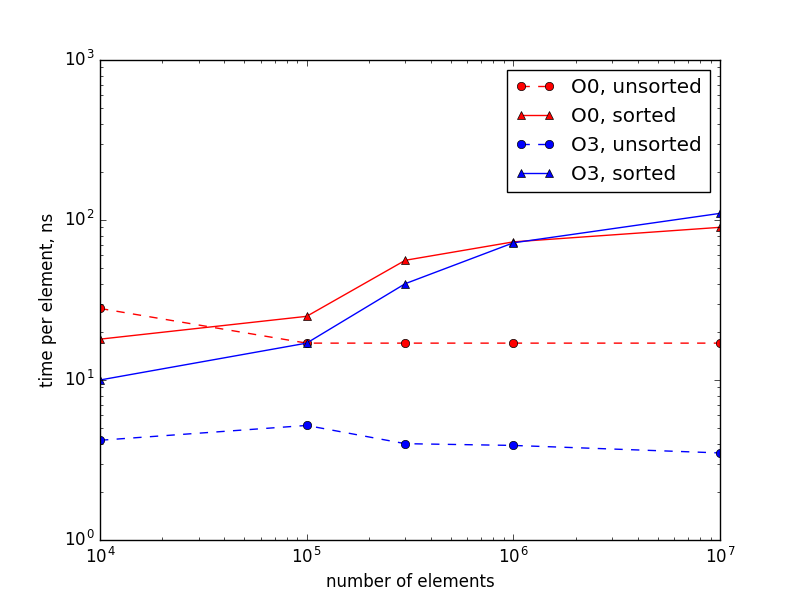
\includegraphics[width=8.3cm]{cache.png}
    \caption{\label{fig:stereo}Time of {\it sum} function.}
\end{figure}

\subsection{Потоки в C++}

Поддержка потоков появилась в стандарте C++ 2011 года, до этого приходилось
пользоваться сторонними библиотеками (например, Pthreads).

Поток (thread) --- наименьшая единица обработки, исполнение которой может быть назначено ядром
операционной системы. Несколько потоков могут существовать в рамках одной и той же программы
(процесса) и иметь общий доступ к её ресурсам.  Потоки могут быть использованы для реализации
одновременности (concurrency; пример --- cin, или приложение с графическим интерфейсом, игровой
сервер), в том числе на одноядерных системах, а также для реальных параллельных вычислений. В
последнем случае потоки выполняются параллельно на разных процессорах (ядрах). Как правило,
необходима синхронизация работы потоков. Синхронизация может быть выполнена с помощью семафоров
(semaphore) и мьютексов (mutex, mutual exclusion) (E.  Dijkstra, 1963 -- 1965).

A parallel program is one that uses a multiplicity of computational hardware (e.g., several
processor cores) to perform a computation more quickly. The aim is to arrive at the answer earlier,
by delegating different parts of the computation to different processors that execute at the same
time.

By contrast, concurrency is a program-structuring technique in which there are multiple threads of
control. Conceptually, the threads of control execute “at the same time”; that is, the user sees
their effects interleaved. Whether they actually execute at the same time or not is an
implementation detail; a concurrent program can execute on a single processor through interleaved
execution or on multiple physical processors.

Работа многопоточной программы является недетерменированной, поэтому
синхронизация крайне важна. Ошибки в многопоточных программах может быть
чрезвычайно трудно <<отлавливать>>, поскольку они, как правило,
невоспроизводимы (см. Therac-25, убрана аппаратная защита, полностью положились на компьютер,
слишком быстрое нажатие кнопки вверх могло привести к переоблучению, поскольку одна и та же
переменная использовалась для чтения чисел и установленной дозы, деление на ноль, синхронизации не
было вообще). Рассмотрим программу:
\begin{minted}{cpp}
  int x = 0;
  ...
  // Поток 1
  x = x + 1;
  // Поток 2
  if (x % 2 == 0)
    std::cout << "x = " << x << '\n';
\end{minted}
Возможны три варианта развития событий, в том числе, программа может напечатать 
\mintinline{bash}{x = 1}. (Состояние гонки, race condition).

Пусть есть переменные $A$ и $S$. Доступ к $A$ возможен только в том случае, если $S
== Green$. В данном примере $S$ является семафором, а $A$ можно рассматривать
как железнодорожную станцию. Поезд, прибывая на станцию, зажигает на путях
красный свет, сигнализируя о том, что пути заняты. Отправляясь от станции, поезд
зажигает зелёный свет. Другим примером использования может быть функция входа в
систему с ограниченным числом пользователей. Пользователь при входе увеличивает
$S$ на единицу, при выходе --- уменьшает, если $S$ больше некоторого значения,
система не пускает новых пользователей.

Мьютексы подобны бинарным семафорам, однако для них определено понятие
владельца, то есть того, кто может переключать состояние. Представьте комнату
--- разделяемый ресурс. Поток, <<заходя>> в <<комнату>>, закрывает за собой
дверь и оставляет ключ в замке. Тогда снаружи никто, даже имея ключ, не может
открыть дверь. И только после того, как поток, находящийся внутри, откроет дверь,
другой поток сможет войти.

Рассмотрим примеры.
\begin{minted}{cpp}
  #include <thread>
  #include <iostream>
  using namespace std;

  void hi(int id) {
      cout << "Thread " << id << " says \'hi!\'\n";
  }

  int main() {
      thread t0(hi, 0);
      thread t1(hi, 1);
      thread t2(hi, 2);
      // threads should be joined or detached, otherwise destruction will
      // terminate the program
      t0.join(); // join function returns when the thread execution has completed
      t1.join();
      t2.join();
      cout << "This is the last message.\n";
      return 0;
  }
\end{minted}
Пример того, что данная программа напечатает:
\begin{minted}{bash}
  Thread 1Thread 0 says 'hi!'
  says 'hi!'
  Thread 2 says 'hi!'
  This is the last message.
\end{minted}
В данном примере синхронизация между порождёнными потоками и основным потором
есть, а порождённые потоки пытаются одновременно получить доступ к устройству
вывода. Синхронизуем с помощью мьютексов.
\begin{minted}{cpp}
  #include <thread>
  #include <iostream>
  #include <mutex>
  using namespace std;

  mutex mtx; // constructor creates mutex in unlocked state

  void hi(int id) {
      mtx.lock();
      cout << "Thread " << id << " says \'hi!\'\n";
      mtx.unlock();
  }

  int main() {
      thread t0(hi, 0);
      thread t1(hi, 1);
      thread t2(hi, 2);
      t0.join();
      t1.join();
      t2.join();
      cout << "This is the last message.\n";
      return 0;
  }
\end{minted}
Пример вывода:
\begin{minted}{bash}
  Thread 0 says 'hi!'
  Thread 2 says 'hi!'
  Thread 1 says 'hi!'
  This is the last message.
\end{minted}
При попытке разблокировать мьютекс потоком, не владеющим им, получаем
непредсказуемый результат.
\begin{minted}{cpp}
  void hello(int id) {
    mtx.unlock(); // undefined behaviour; mutex should be locked by this thread before
    cout << "Thread " << id << " says \'hello!\'\n";
  }
\end{minted}
Если хотим вывести сообщения последовательно, в соответствии с id --- тогда
следует завести массив мьютексов.

<<Подводные камни>>. Во-первых, потоки нельзя копировать, поскольку они
соответствуют реальным нитям исполнения, и копирование для них ---
неопределённая операция (копирование происходит, например, при передаче объекта
в функцию). Во-вторых, при передаче аргументов функции потока через конструктор
\mintinline{cpp}{thread()} происходит копирование аргументов, поэтому
использовать ссылки в качестве аргументов напрямую нельзя. Рассмотрим пример:
\begin{minted}{cpp}
  #include <iostream>
  #include <vector>
  #include <thread>

  using namespace std;

  // thread function, changes x[id]
  /* thread() copies arguments, thus we shoud use pointer instead of reference */
  void f(vector<int>* x, int id) {
    (*x)[id] += 1;
  }

  int main(){
    vector<int> x;
    vector <thread> v(5);
    for (auto it = v.begin(); it != v.end(); ++it) {
      static int id = 0;
      x.push_back(0); // ERROR: pointer to vector can be changed by push_back
      *it = thread(f, &x, id);
      ++id;
    }
    /* thread objects cannot be copied, so this causes an error:
    for (auto x : v)
      x.join();
    but this is ok:
    for (auto& x : v)
      x.join();
    */
    for (auto it = v.begin(); it != v.end(); ++it)
      it->join();
    for (auto y : x) {
      static int i = 0;
      cout << "x[" << i << "] = " << x[i] << '\n'; // 1 1 1 1 1
      ++i;
    }
    return 0;
  }
\end{minted}

\section{Openmp}

Недостатки программы с C++11 threads: не везде есть поддержка стандарта (потоки --- разные, трудно
писать кроссплатформенные приложения), скомпилировать программу без потоков нельзя (для
какого-нибудь утюга с малой памятью итп), сложная логика, синхронизация и т. п., большая зарплата
программистов.

\begin{figure}
  \centering
  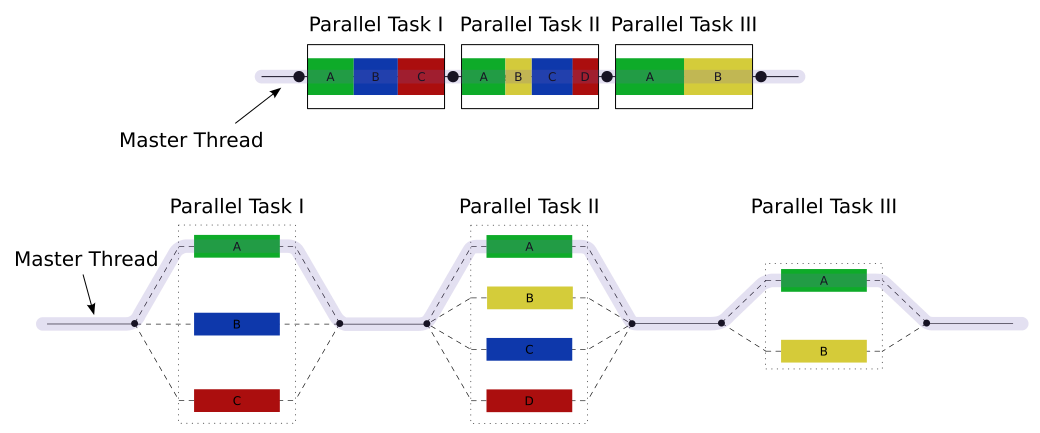
\includegraphics[width=12cm]{Fork_join_omp_wiki.png}
  \caption{\label{fig:mathgl_stereo}Master thread forks and joining tasks.}
\end{figure}

OpenMP (Open Multi-Processing) предоставляет как библиотечные функции для работы
с потоками, так и директивы компилятора --- прагмы (pragmatic information).
Прагмы обрабатываются препроцессором или компилятором. Если компилятор не
понимает директивы --- он её игнорирует, что очень удобно для создания
переносимых программ. Рассмотрим примеры.

\begin{minted}{cpp}
  #include <iostream>
  #include <omp.h>
  using namespace std;

  int main(){
    #pragma omp parallel /* -> fork additional threads only for enclosed work */
    cout << "Hello, world!\n";
    cout << "Hi, Universe!\n";
    return 0;
  }
\end{minted}
Результат для двухъядерного процессора:
\begin{minted}{bash}
  Hello, world!
  Hello, world!
  Hi, Universe!
\end{minted}
--- по числу ядер, но синхронизации нет, может быть смешение в первых двух
строчках.

В качестве примера посложнее рассмотрим заполнение массива. При заполнении все
элементы независимы, спокойно можем делать в нескольких потоках.

\begin{minted}{cpp}
  #include <iostream>
  #include <omp.h>
  using namespace std;

  const int number_of_threads = 4;
  const long n = 1000;

  int main(){
    omp_set_num_threads(number_of_threads);
    double* a = new double[n];
    #pragma omp parallel for // team of threads processing the loop
    for (long i = 0; i < n; ++i) {
      a[i] = i;
    }
    for (long i = 0; i < n; ++i) { // this loop processed by the master thread
      cout << a[i] << ' ';
    }
    cout << '\n';
    delete[] a;
    return 0;
  }
\end{minted}

Если бы мы заполняли вектор с помощью pushback, могли бы нарваться на ошибки.
Однако можно создать вектор из имеющегося массива, а можно и выделить память под
вектор большой длины, а потом его заполнять.

Как быть с обменом? Попробуем написать reduce. Map и reduce --- две
знаменитые абстрактные функции, пришедшие из функционального программирования.

\begin{minted}{cpp}
  #include <iostream>
  #include <omp.h>
  #include <chrono>
  using namespace std;

  // 'greedy' reduce
  // !!! parallel version, can be used only for commutative operation f !!!
  template<typename T> T reduce(T f(T, T), T r0, T* a, long n) {
    T rsh = r0;
    T rpr;
 /* team of threads is created here;
    `rsh` is visible and accessible by all threads simultaneously;
    `rpr` is used as a temporary variable (local copy)
 */
    #pragma omp parallel shared(rsh) private(rpr)
    {
      rpr = 0;
      #pragma omp for
      for (long i = 0; i < n; ++i)
        rpr = f(rpr, a[i]);
      // the following section is executed only by one thread at a time
      #pragma omp critical
      rsh += rpr;
    }
    return rsh;
  }

  double sum(double a, double b) {
    return a + b;
  }

/* for the task about a sequence with all numbers repeated twice but one is unique
  int fxor(int a, int b) {
    return a^b;
  }
*/

  const int number_of_threads = 4;
  const long n = 1000000;

  int main(){
    omp_set_num_threads(number_of_threads);
    double* a = new double[n];
    #pragma omp parallel for // team of threads processing the loop
    for (long i = 0; i < n; ++i)
      a[i] = i + 1;
    auto start =  chrono::high_resolution_clock::now();
    cout << reduce<double>(sum, 0, a, n) << '\n'; // (n * n - n) / 2 + n = (n^2 + n) / 2
    auto end =  chrono::high_resolution_clock::now();
    cout << static_cast<double>((n * n + n) / 2) << '\n';
    cout << "reduce takes = " << (chrono::duration_cast <chrono::nanoseconds> (end - start)).count() << " ns\n";
    delete[] a;
    return 0;
  }
\end{minted}

\subsubsection{Задача (7 баллов, 14 Oct, 3 б за правильный ответ, оценка шага 1 б, время 1 б,
опенмп и график времени от числа потоков 2 б.)}

Исходные тексты (.cpp, .hpp) посылайте на nerush\_at\_appl.sci-nnov.ru. Баллы
держатся 2 недели, потом убывают на 1 балл в неделю.

Задача: вычислить методом прямоугольников в средней точке следующий интеграл:
\begin{equation}
  \int_0^{(31 \pi /2)^{1/3}} 3 x^2 \sin (x^3) \, dx
\end{equation}
\begin{enumerate}
  \item Использование OpenMP приветствуется. % +1
  \item Программа должна выводить правильный ответ в консоль. % +3
  \item Оценка шага интегрирования приветствуется. % +1
  \item Вывод времени интегрирования и график (число потоков, время). % +2
\end{enumerate}

\subsection{Message Passing Interface (MPI)}

Поток --- наименьшая единица обработки, испольнение которой может быть назначено
ядром операционной системы. Поток находится внутри процесса. Процесс ---
программа, которая выполняется в текущий момент (включая адресное пространство,
стек, глобальные переменные и т. п.). Потоки <<видят>> общие переменные
программы и могут их использовать. В то же время при попытке доступа к <<чужой>>
памяти из программы произойдёт SegFault. Для общения между процессами служит
стандарт MPI (существует 2 реализации --- openMPI и mpich2).

MPI позволяет создать $n$ копий одной и той же программы, отличающихся id. Число программ не
изменяется во вроемя выполнения, обмен --- только за счёт пересылки сообщений. MPI стоит
использовать, даже если вы пишите приложение под одну машину --- сильной потери скорости по
сравнению с потоками и разделяемой памятью скорее всего не будет. Ограничения на обмен на самом
деле упрощают написание программы и избавляют от ошибок. Программа с самого начала разделена на
независимые части. Однако фиксированное число процессов может быть неудобно.  Есть синхронизация и
т. д. Пример с движением большого числа частиц. А что делать, если они взаимодействуют? Работает
часто не медленнее потоков, накладные расходы невелики. Главный плюс --- работает на системах с
распределённой памятью --- часть задач может быть на одном компьютере, часть --- на другом.

\section{OpenCL, CUDA.}

Graphics Processing Unit (GPU) --- процессор видеокарты. Используются для
текстурирования трёхмерных объектов и т. п. Поскольку типичные задачи ведеокарт
хорошо распараллеливаются, число ядер в них, как правило, $\gg 1$. Ядра,
организация памяти
и т. п. могут сильно отличаться от ядер CPU и оперативной памяти в компьютере,
но способны проводить вычисления с плавающей точкой (обычно float, double
медленнее, если есть). Таким образом, некоторые вычисления можно переложить на
GPU.

CUDA (2007) --- Compute Unified Device Architecture, даёт разработчику доступ к
набору инструкций графического ускорителя и к управлению его памятью.
Реализация --- упрощённый диалект C. nVidia only.

OpenCL (2009) --- Open Computing Language --- платформа для написания
компьютерных программ, связанных с параллельными вычислениями, на различных
устройствах. AMD, nVidia, Intel (phi), etc. Позволяет писать программы на С (с
определёнными дополнениями). Из-за общности (для любых устройств) обладает
моделью памяти, отличной от CUDA, из-за чего, как правило, её код работает на
(говорят) 20 процентов медленнее. Одгако может работать как с проприетарными,
так и с открытыми драйверами.

Изначальная идеология: один и тот же код под все устройства, CPU, GPU. Однако
критические места --- разные, и для получения максимальной производительности
нужно модифицировать код.

OpenCL архитектура.

Compute device --- CPU, GPU, ... compute units, processing elements. Kernel runs
on PEs in parallel. Compute unit не обязательно равно core. Модель памяти:

global memory: shared by all processing elements, but has high access latency;

read-only memory: smaller, low latency, writable by the host CPU but not the
compute devices;

local memory: shared by a group of processing elements;

per-element private memory (registers).

Работает чрезвычайно быстро, может на ноутбучной видеокарте обогнать процессор в
несколько раз даже при простой архитектуре приложения.

\subsection{Блокчейн, криптовалюты, биткоин (BTC)}

Хэш (hash, хэш-сумма).

Хэш-функция переводит массив из бит (файл, структуру в памяти, или просто кусок памяти) в число
(обычно фиксированной длины, 256 бит, например). На неё накладывается два очень важных условия,
которые говорят о её "непредсказуемости":

1) Для массивов, отличающихся даже на 1 бит, хэш-суммы должны значительно отличаться.

2) Не существует (или хотя бы неизвестен) алгоритм, позволяющий сгенерировать файл, дающий наперёд
заданную хэш-сумму.

Таким образом, вероятность того, что хэш какой-то структуры (или массива и т. п.) попадёт в наперёд
заданный узкий интервал, будет маленькой. Одна из самых известных хэш-функций - sha256

Хэш-чеин (hash chain).

Помните, как устроен односвязный список? Каждый элемент списка помимо значения хранит указатель
(адрес) следующего элемента списка, тот - следующего за ним, и так до конца. Блокчеин в простейшем
виде - тот же односвязный список, но в нем каждый следующий элемент ещё хранит хэш предыдущего
элемента. При этом этот хэш считается от всего элемента, включая ту часть, в которой записан хэш
элемента перед предыдущим.

Если в обычном списке замена элемента обойдётся в O(1) операций, то в таком простейшем блокчеине
для замены элемента нужно будет вычислить заново и записать хэш-суммы всех последующих элементов,
стоить это будет O(N).

Дерево Меркла

Теперь представим двоичное дерево, построенное по несколько похожему принципу. Пусть нижние ноды
дерева содержат хэши данных (разбитых на блоки), для этих нод попарно вычисляется хэш от суммы (или
объединения) их хэшей, и так далее, до верхушки. Построение такой структуры выполняется за O(N)
операций, однако изменение одного блока данных и перестройка дерева будет стоит O(log N). Проверка
того, что данный блок принадлежит дереву, также дешёвая - для этого достаточно посчитать хэш блока
и пройтись по нодам снизу вверх, за O(log N).

Proof-of-work

Bitcoin хранит транзакции в дереве Меркла. Транзакции - это переводы средств с одного адреса на
другой. Очевидно, в этой сети можно легко проверить, что транзакция записана верно, просто вычислив
цепочку хэшей длиной O(log(N), идя по дереву снизу вверх. Но возникает некоторая проблема - в
дереве Меркла переписать цепочку нод так же легко. Для того, чтобы переписать или изменить что-либо
в дереве было практически невозможно, дерево Меркла строится на основе блокчейна.

Блокчейн (blockchain, цепочка блоков) - это тот же хэшчейн (на самом деле часто и то и другое
называют блокчейном), но каждый элемент списка имеет определённое поле, в котором может быть
записано что угодно, а на хэши накладывается условие, обеспечивающее сложность вычислений:
например, требуется, чтобы хэш-сумма не превышала определённого значения. Меняя данные в поле для
произвольных данных, и пересчитывая хэш, можно подобрать содержимое этого поля таким, что условие
будет выполнено.

Если пороговое значение для хэша не очень большое, то подбирать данные для произвольного поля
придётся достаточно долго. В то же время на сложности проверки блокчейна все эти условия и
дополнительные поля никак не сказываются.

Майнинг - это и есть перебор чисел в свободном блоке и вычисление хэшей. Поскольку эта операция
затратная, но необходимая для работы сети (без неё не записать транзакции), то он оплачивается -
теми же биткоинами.

\subsection{Сортировка слиянием.}

Существует множество методов сортировки, среди которых нет <<лучшего>>. Выбор
метода может зависеть от свойств набора данных. Свойства метода сортировки:
необходимое время и объём памяти, устойчивость.

Наверное, самый простой способ сортировки --- создать ещё один массив нужной длины, и заполнять его
по порядку минимальными элементами из сортируемого массива (заменяя при этом сами минимальные
элементы на число, большее максимального).
 
Пузырьковая сортировка (bubble sort). Алгоритм: меняем местами соседние элементы
сортируемого массива по принципу <<меньший --- налево>> до тех пор, пока таких
замен при проходе массива не придётся делать (массив стал упорядоченным).
Требует $O(1)$ памяти и может быть устойчив (безопасен), но время выполнения
$O(n^2)$ для массива из $n$ элементов.

Insertion sort iterates, consuming one input element each repetition, and growing a sorted output
list. Each iteration, insertion sort removes one element from the input data, finds the location
it belongs within the sorted list, and inserts it there. It repeats until no input elements
remain. Легко представить алгоритм с потреблением памяти $O(1)$ (in-place алгоритм, слева
сортированный массив, справа --- несортированный).

Быстрая сортировка (quick sort или qsort, T. Hoare, 1959). Алгоритм:
\begin{enumerate}
  \item Выбираем некоторое число-разделитель.
  \item Делим массив на два массива: один из чисел меньших числа-разделителя,
    другой --- из больших или равных.
  \item Для каждого из полученных массивов выполняем первые два пункта.
  \item Очевидным образом соединяем полученные массивы в один.
\end{enumerate}
Пример кода на Haskell:
\begin{minted}{haskell}
qsort []     = []
qsort (x:xs) = qsort lhs ++ [x] ++ qsort rhs
    where lhs = filter  (< x) xs
          rhs = filter (>= x) xs
\end{minted}
Доказательство очевидно. Может быть безопасной. В среднем требует $O(n\log n)$ сравнений элементов
("времени"), однако в некоторых случаях время выполнения $O(n^2)$. Например, в случае, если в
качестве элемента-разделителя выбирается среднее значение элементов массива, а элементы
распределены с плотностью $f(x) \sim 1 / \sqrt{x}$. Проблема повторяющихся элементов, решение: делить на три
части и не делать qsort для средней, $[x,x,x,x]$ (то есть для разделения использовать солвер
проблемы национального голландского флага). Если разделитель выбирать случайным, вероятность
попасть на неоптимальное распределение довольно мала.
Требует в простейшей реализации $O(n)$ памяти (может быть улучшена до
$O(\log n)$: сначала рекурсия (требует на каждом шаге хранение постоянного объёма аргументов
вызываемой функции, что приводит к потреблению памяти $O(\log(n))$, а для оставшихся коротеньких
массивов можно применить bubble sort, потребление памяти которым может быть сведено к минимуму).

Иногда просто её реализация оказывается
быстрее, чем msort (небезопасная примерно вдвое быстрее, чем msort).

Сортировка слиянием (merge sort, J. von Neumann, 1945). Алгоритм:
\begin{enumerate}
  \item Разделить массив на $n$ массивов из одного элемента.
  \item Объединять массивы, сравнивая <<головы>> массивов и <<отщипывая>>
    минимальный элемент. Повторять этот шаг до тех пор, пока не получится один
    массив, который окажется отсортированным.
\end{enumerate}
Код (Haskell):
\begin{minted}{haskell}
join [] a = a
join a [] = a
join (y:ys) (z:zs)
    | y < z     = y : (join ys (z:zs))
    | otherwise = z : (join (y:ys) zs)

split [] = ([], [])
split [u] = ([u], [])
split (v:w:ts) = (v:vs, w:ws)
    where (vs, ws) = split ts

msort :: [Int] -> [Int]
msort [] = []
msort [x] = [x]
msort x = join (msort lhs) (msort rhs)
    where (lhs, rhs) = split x
\end{minted}
Доказательство --- по индукции. В случае слияния массивов из одного элемента
получатся упорядоченные массивы из двух элементов. Теперь предположим, что
происходит слияние упорядоченных массивов из нескольких элементов. В
массив-результат мы всегда добавляем меньший элемент из исходных массивов,
значит, он меньший и в объединённом массиве.

Данный алгоритм затрачивает $O(n)$ памяти и $O(n\log n)$ времани на сортировку.

Heapsort. Williams, 1964.


functionnal init, xcels example

\subsection{SO3}

\section{Второй курс}

Параллелелизм в котлин, питон?

\subsection{О линейной алгебре и теории групп}

Рассмотрим задачу из книги~\cite{Kirillov08} (Example 1.1), кажущуюся на первый взгляд чисто
практической, но имеющую очень красивое математическое решение. Пусть у нас есть комплексные числа $a_1, ...,
a_n$, и есть преобразование $A$, заменяющее $a_1$ на $(a_n + a_2) / 2$, $a_2$ на $(a_1 + a_3) /
2$ и т.~д. Если много раз применить преобразование $A$, что в итоге получится?

Для ответа нужно найти собственные значения оператора $A$, однако явное вычисление корней
характеристического многочлена --- непростая задача. Тем не менее можно заметить, что задача
обладает вращательной симметрией. Введём оператор $B$ такой, что он делает "вращение" на $2 \pi
/ n$, а именно посылает числа $a_1, a_2, ..., a_n$ в ячейки $a_2, a_3, ..., a_1$. Очевидно, что
$B A B^{-1} = A$, то есть $A$ и $B$ коммутируют.

Оператор $B$ порождает группу, изоморфную группе $\mathbb Z_n$ (группа целых чисел ${0, 1, ..., n -
1}$ со сложением по модулю $n$). Как можно использовать эту группу для поиска собственных
векторов оператора $A$? Можно использовать хорошо известный из линейной алгебры результат: если
$A$ и $B$ коммутируют в векторном пространстве $V$, и $V_\lambda$ есть линейное
подпространство, соответствующее некоторому собственному числу $\lambda$ оператора $B$, то $A
V_\lambda \subset V_\lambda$ (легко доказать "от противного"). Следовательно, если оператор $B$
диагонализуем так, что исходное векторное пространство раскладывается в прямую сумму $V =
\bigoplus V_\lambda$, тогда $A$ сохраняет эту декомпозицию и задача сводится к диагонализации
$A$ отдельно в каждом из $V_\lambda$, что существенно проще.

\textit{Задача для решения у доски.} Можно заметить, что $B^n = \mathrm{id}$ (единичный оператор), следовательно, все
собственные значения $B$ есть $n$-ые корни мнимой единицы. Показать, что все собственные значения
различны, найти их, найти собственные вектора (они же собственные вектора $A$!) и найти собственные
значения $A$. Что будет с $(a_1, ..., a_n)$ при многократном применении $A$?

\subsection{Повторение}

int main. const. static. Структуры. Шаблоны. Шаблоны с числовым параметром (non-type template parameter). Классы.
Наследование. 
Структурирование кода. Функции, передача функций в качестве аргумента. Top-down method. 

Стандартная библиотека. Vector, List, Map. Размещение в памяти. $O(N)$ нотация и стоимость операций
вставки, удаления. Сбалансированные деревья. Сортировка быстрая, слиянием.

потоки. OpenMP, MPI, OpenCL

\subsection{Интегрирование методом Монте-Карло}

Феномен Пиаже (как комментарий к задаче Кириллова). А какик собственные вектора у оператора,
который локально заменяет $a_2$ на $3 a_1 + a_4$, и т. д.? Наше пространство симметрично
относительно трансляций, оно одно и тоже в разных точках, поэтому симметрия в физических задачах
оказывается так важна.

\subsection{Методы генерации случайных чисел с заданным распределением}

\subsubsection{Rejection sampling (выборка с отклонением, или с отбраковкой)}

\begin{figure}
	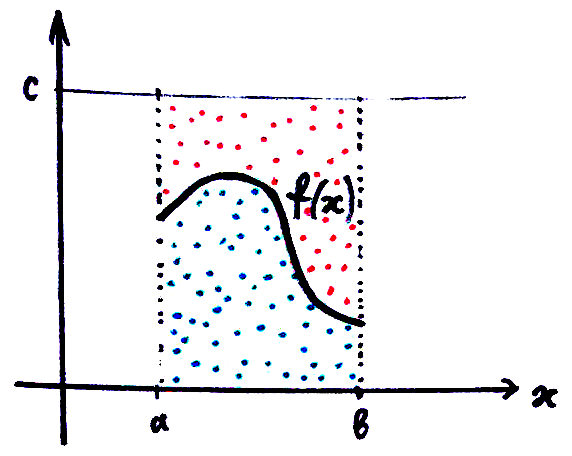
\includegraphics[width=0.6\linewidth]{rejection-sampling.png}
    \caption{\label{dots-for-monte-carlo}Rejection sampling: точки под кривой (синие) имеют
    распределение $dN/dx = f(x)$.}
\end{figure}

Этот метод является очень простым, и в то же время имеет много общего с геометрическим методом
Монте-Карло для вычисления интегралов. Суть его простейшего варианта в следующем. Предположим, что
мы умеем генерировать числа, равномерно распределённые на отрезке $(a, b)$, но нам нужен генератор
псевдослучайных чисел, имеющих распределение $dN/dx = f(x)$ на этом отрезке. Таким образом,
вероятность попадания числа в интервал $(x, x + \Delta x)$ для $\Delta x \to 0$, должна быть
пропорциональна $f(x)$.  Считаем, что $f(x)$ ограничена, то есть $f(x) < c$ [также очевидно, что
$f(x)$ не может быть меньше нуля]. Тогда мы можем равномерно засеять область $x \in (a, b)$, $y \in
(0, c)$ случайными точками, и отбраковать (отклонить) те из них, которые окажутся над кривой $f(x)$.
Оставшиеся точки будут иметь нужное нам распределение!

Для доказательства найдём число точек, попадающих в среднем в интервал $(x, x + \Delta x)$ при
малом $\Delta x$. Поскольку распределение точек на интервале $(a, b)$ до отбраковки равномерное, то
их число (опять же, до отбраковки) в интервале $(x, x + \Delta x)$, будет пропорционально $\Delta
x$ и не будет зависеть от $x$. После отбраковки число точек уменьшится в $c / f(x)$ раз, то есть
число оставшихся в интервале $(x, x + \Delta x)$ точек пропорционально $f(x)$, что и требовалось
доказать. Остаётся только отметить, что при программировании данного метода отбраковку точки можно
производить сразу же по критерию $y_j > f(x_j)$, без сохранения всех точек в какие-либо временные
структуры.

\subsubsection{Обращение $N(x)$}

\begin{figure}
	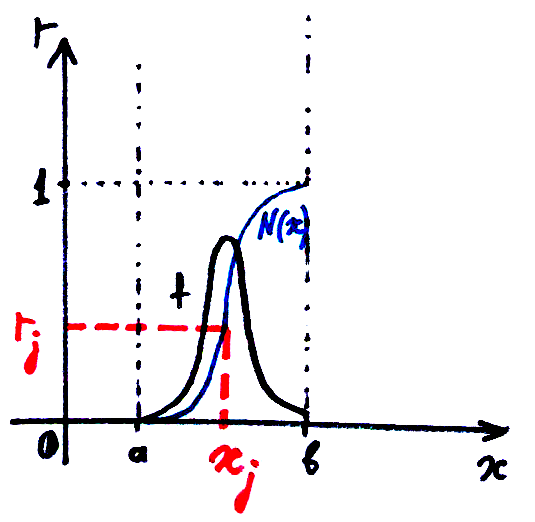
\includegraphics[width=0.6\linewidth]{inversion-of-N.png}
    \caption{\label{dots-for-monte-carlo}Генерация случайных чисел с использованием обратной
    функции для N(x).}
\end{figure}

Для заданного распределения $dN/dx = f(x)$ на отрезке $[a, b]$ можно ввести функцию
\begin{equation}
    N(x) = \int_a^x f(x') \, dx',
\end{equation}
при этом мы считаем, что $f(x)$ нормирована таким образом, что $N(b) = 1$. Для простоты будем
считать, что не существует интервалов, не которых $f(x) \equiv 0$, тогда $N(x)$ --- монотонно
растущая функция, и существует однозначная обратная функция $\tilde N(r)$ \{$r \in [0, 1]$\}
такая, что
\begin{equation}
    \label{tilde_N_N}
    \tilde N(N(x)) = x.
\end{equation}

Если $\tilde N(r)$ может быть найдена в аналитической форме, то распределение точек $x_j = \tilde
N(r_j)$ пропорционально $f(x)$, при условии, что случайные числа $r_j$ имеют равномерное
распределение на отрезке $[0, 1]$. Для доказательства рассмотрим бесконечно малый интервал $[r, r +
\Delta r]$, и обозначим число точек $r_j$, попавших на этот интервал, $\Delta N$.
Интервалу $\Delta r$ соответствует
\begin{equation}
    \Delta x = \tilde N(r + \Delta r) - \tilde N(r) \propto \frac{d \tilde N}{dr} \propto \left(
    \frac{dN}{dx} \right)^{-1} = \frac{1}{f(x)},
\end{equation}
где мы использовали уравнение~(\ref{tilde_N_N}), продиффиренцированное по $x$.
В силу равномерного распределения чисел $r_j$ имеем $\Delta N /
\Delta r = \mathrm{const}$ (то есть не зависит от $r$), следовательно, $\Delta N / \Delta x \propto f(x)$, что и требовалось
доказать.

Рассмотрим пример. Пусть нам требуется сгенерировать числа, имеющие распределение $f(x) = 2 x$ на
отрезке $[0, 1]$. В этом случае $N(x) = x^2$, и для получения точек, имеющих распределение $f$,
нужно применить к равномерно распределённым точкам $r_j$ функцию $\tilde N(r) = r^{1/2}$. Очевидно,
основным недостатком данного метода является невозможность нахождения в аналитической форме функции
$\tilde N$ в большинстве случаев.

\textit{Вопрос.} Какой алгоритм следует использовать для генерации псевдослучайных чисел с
распределением (а) $f(x) = 1 / x^{1/2}$, (б) $f(x) = \cos (x^2)$, (в) $f(x) = 1 / x$  на интервале
$(0, 1)$, а также для (г) $f(x) = \exp(-x^2)$, $x \in (-\infty, \infty)$?

\textit{Задача}. (Kotlin!) Cгенерировать массив наперёд заданной длины из псевдослучайных чисел с
функцией распределения либо
\begin{equation}
    \frac{dN}{dx} \propto \exp(\sin(\pi x^2)), \qquad x \in (0, 1),
\end{equation}
либо
\begin{equation}
    \frac{dN}{dx} \propto 1 / x^{1/2}, \qquad x \in (0, 1).
\end{equation}
Продемонстрировать корректность работы генератора:
\begin{enumerate}
  \item Найти и вывести на экран <<центр масс>> полученного распределения (среднее значение $x$,
      должно получиться 0.561418 в первом случае и $1/3$ во втором случае).
  \item Найти функцию распределания чисел, раскидав сгенерированные числа по
      корзинкам, и сравнив с теорией на графике.
\end{enumerate}
Задачу выполнять группами по 4 человека, каждый отвечает за свою часть кода: генерацию
распределения (того или другого), вычисление среднего, вычисление и построение функции
распределения.

\subsubsection{Why Kotlin?}

Какое отношение Kotlin имеет к научному программированию? Почему мы почти не будем изучать гораздо
более распространённый в научной среде Python? Дело в том, что программирование (научное в том числе) - это не
только написание своего кода, но и взаимодействие с коллегами (умение объяснять, чтение чужого кода
и документации, код-ревью), рефакторинг (то есть улучшение кода без изменения его
функциональности), поддержка и тестирование, работа с системами контроля версий. Учиться этим
аспектам лучше на новых платформах: они удобнее, проще для освоения, они позволяют хотя бы мельком
взглянуть на новые возможности (более понятные сообщения об ошибках, помощь в рефакторинге и т.
п.), они могут быть избавлены от старых ошибок. Python в этом смысле не очень подходит. Его
дополнительная проблема состоит в том, что многие легко осваивают простейшие операции и пару библиотек (numpy,
matplotlib) и им кажется, что изучение Python на этом можно закончить. Низкий порог входа отбивает
желание двигаться дальше. Динамическая типизация также даёт ложное ощущение простоты. Kotlin лишь
за счёт статической строгой типизации и вывода типов позволяет избежать множества ошибок, легко
проникающих в программу, написанную на Python. Kotlin поддерживает pattern matching (сопоставление
с образцом) и другие особенности функционального программирования гораздо лучше, нежели Python...
Таким образом,  мы сосредоточимся на  самой сути программирования, и отсутствие для Kotlin хороших
библиотек для численного решения дифференциальных уравнений не будет для
нас проблемой. Кроме того, Kotlin, кажется, имеет высокую производительность и вполне подходит для
научного программирования. А Matplotlib и Scipy для Python читатель может изучить самостоятельно.

%tdd, командные задачи Объём шара. ГСЧ, функция-фильтр (внутри-снаружи, от функции-условия, то есть
%не только для шара), график от размерности. Тесты, презентация проекта? github. Рефакторинг - 1) на
%произвольную форму, 2) параллелелизм.  идеи. паттерн матчинг, полиморфизм, typeclasses?,  lazy
%evaluations. func chain тест вейля, свойство гспч продолжать с середины

\subsubsection{Промежуточное представление и виртуальная машина}

Создание компилятора (преобразующего исходный код в машинный код) - сложная задача. В начале
компьютерной эры под каждую новую платформу (со своей особенной архитектурой) приходилось писать
свой компилятор, что отнимало много времени и сил. Для решения этой проблемы была предложена идея
промежуточного представления (intermediate representation). При этом компилятор состоит из двух
частей. Первая из исходного кода генерирует код на достаточно простом промежуточном языке. Вторая
часть транслирует промежуточный код (байт-код) в машинный код. Впервые эта идея была реализована
для языка BCPL около 1967 года, за счёт чего при портировании компилятора на новую платформу
приходилось переписывать лишь $1/5$ часть его кода.

Впоследствии эта идея получила очень широкое распространение. Кроме простоты портирования
компиляторов, использование промежуточного представления позволяет отвязать исходный
высокоуровневый язык от конкретной ахитектуры. Например, можно ``постановить'', что Int -
целочисленный тип длиной 32 бита, а Long - 64 бита (я думаю, читатель помнит, что в C++ для int и
long определены лишь верхний и нижний пределы их длины, а не их длина в точности). При этом
реализация этих типов на конретной архитектуре осуществляется при написании второй части
компилятора, переводящего байт-код в машинный код.

Вместо второй части компилятора можно использовать интерпретатор, который покомандно (построчно)
выполняет байт-код. Такой интерпретатор называется виртуальной машиной (virtual machine).
Интерпретатор, как правило, легче реализовывать, кроме того, он, например, может проверять
корректность ссылок (на этапе компиляции реализовать такую проверку можно далеко не всегда).
Подобным образом - за счёт дополнительных проверок - Java virtual machine (JVM) защищает данные от
случайного повреждения, а саму себя - от падения. Язык Kotlin создавался для компиляции в байт-код
JVM, хотя может компилироваться в машинный код через промежуточное представление LLVM.

скорость работы...

\subsubsection{Kotlin basics}

Kotlin --- язык программирования, разрабатываемый компанией JetBrains, компилируемый в байт-код для
Java virtual machine. Самый простой способ начать его осваивать --- установить среду разработки
(Integrated development environment, IDE) Intellij IDEA и создать в ней новый проект. После её установки потребуется либо
скачать Java SDK из интерфейса Intellij IDEA (File -> Project Structure -> SDKs -> +), либо
установить Java SDK самостоятельно и указать путь к нему в том же интерфейсе. Точкой входа в
программу на языке Kotlin является функция main, поэтому простейшая программа может состоять из
одного файла (для его создания можно кликнуть правой кнопкой мыши директорию src в проекте, и далее
выбрать New -> Kotlin File -> hw; будет создан файл hw.kt), содержащего следующий код:
\begin{minted}{kotlin}
    fun main() {
        println("Hi, world!")
    }
\end{minted}
Для компиляции и выполнения программы достаточно нажать Shift+F10.

Kotlin --- статически типизированный язык, тип переменных необходимо либо указывать явно после
двоеточия, либо не указывать --- если его можно вывести из выражения. Переменные могут быть
объявлены read-only константами (val), либо быть действительно переменными (var). Рассмотрим
примеры, поясняющие основы синтаксиса языка Kotlin.
\begin{minted}{kotlin}
    val a: Int = 1 // const; 32-bit signed integer
    val b: Double = 3.14 /* const; double-precision
                            64-bit IEEE 754 floating point number */

    var c = 3 // `Int` type is inferred
    c += 1    // can be reassigned (var)

    // sum of arguments
    fun sum(a: Int, b: Int): Int {
        return a + b
    }

    // use `Unit` instead of `void`
    fun printSum(a: Int, b: Int): Unit {
        // `println` adds line break, while `print` doesn't
        println("sum of $a and $b is ${a + b}") // look at this!
    }

    // in Kotlin, `if` can also be used as an expression;
    // and function can set with =
    fun maxOf(a: Int, b: Int) = if (a > b) a else b

    // classes, inheritance, templates are also available in Kotlin...
\end{minted}

Для работы с массивами (списками, деревьями...) в Kotlin реализованы необходимые структуры данных
(коллекции). Одной из простейших структур является List - неизменяемая (immutable) структура данных
с возможностью доступа по индексу. Для изменяемых массивов данных (с изменяемым размером) можно
использовать MutableList. Если требуется гарантия быстрого доступа по индексу, то следует
использовать ArrayList (в каком-то смысле это аналог std::vector из C++). Рассмотрим примеры:
\begin{minted}{kotlin}
fun main() {
    val xs = listOf(1, 4, 2, 7) // immutable
    println(xs[0]) // 1
    println(xs.indexOf(7))  // 3
    println(xs.indexOf(25)) // -1

    for (x in xs) {
        print("$x\t") // 1 4 2 7
    }
    println()
}
\end{minted}

\begin{figure}
	\includegraphics[width=1\linewidth]{LetsPlotExample.png}
    \caption{\label{LetsPlotExample}Простейший график, построенный с помощью lets-plot.}
\end{figure}

Для выполнения задачи понадобится работа со случайными числами и построение графиков, поэтому будет
полезно рассмотреть следующий пример (результат работы которого - на
рисунке~\ref{LetsPlotExample}):
\begin{minted}{kotlin}
import jetbrains.letsPlot.export.ggsave // IDEA сама подсказывает,
                                        // какие модули нужно импортировать
import jetbrains.letsPlot.geom.geomPoint
import jetbrains.letsPlot.letsPlot
import kotlin.random.Random

fun main() {
    val n = 5000
    val gen = Random(12345) // seeded
    var xs: ArrayList<Double> = ArrayList(n) // lists cannot be declared
                                             // without initialization
    var ys: ArrayList<Double> = ArrayList(n)

    for (i in 1..n) { // `1..n` is a Range
        xs.add(gen.nextDouble())
        ys.add(Math.pow(gen.nextDouble(), 2.0))
    }

    val data = mapOf<String, Any>("x" to xs, "y" to ys)

    val fig = letsPlot(data) + geomPoint(
        color = "dark-green",
        size = 1.0
    ) { x = "x"; y = "y" }

    ggsave(fig, "LetsPlotExample.png")
}
\end{minted}

Для компилации последнего примера в проект требуется добавить зависимости (File -> Project Settings
-> Modules -> Dependencies -> + -> Library -> From Maven):
org.jetbrains.lets-plot:lets-plot-kotlin-jvm и org.jetbrains.lets-plot:lets-plot-image-export. 
Подробнее использование библиотеки lets-plot мы рассмотрим чуть позже.

\subsubsection{Алгоритм Метрополиса}

Во многих случаях при генерации случайных чисел с целевой функцией $dN/dx = f(x)$ ни аналитическая
форма, ни общий вид функции $f$ не известены, кроме того, функция $f$ может содержать особенности,
а $x$ может быть вектором многомерного пространства. Мы позже будем
рассматривать пример, в котором $x$ есть траектория частицы (то есть лежит в пространстве функций
--- бесконечномерном), а $f$ определяется действием (то есть некоторым интегралом от траектории).
Очевидно, что в этом случае ни метод выборки с отбраковкой, ни тем более метод с обращением $N(x)$
неприменимы. Тем не менее, есть простой метод, предложенный N.~Metropolis, A.~Rosenbluth,
M.~Rosenbluth и E.~Teller в 1953 году (для краткости --- алгоритм Метрополиса), и подходящий для
чрезвычайно широкого класса $f(x)$.

В алгоритме Метрополиса последовательность случайных чисел генерируется с использованием
цепей Марковa, то есть последовательности случайных состояний, в которой вероятность наступления
состояния зависит от предыдущего состояния. Пусть, например, случайная величина $x$ может принимать
два значения, $+1$ и $-1$. Однако, мы можем представить систему, в которой вероятность того или
иного следующего состояния
системы, $x_i$, зависит от предыдущего, $x_{i - 1}$, например, при $x_{i - 1} = -1$ вероятность
того, что <<выпадет>> $x_i = -1$, равна $1/4$, а при $x_{i - 1} = +1$ эта вероятность равна $1/2$.
Несмотря на такую зависимость вероятности состояний, последовательность чисел $x_0, x_1,...$ будет,
очевидно, случайной.

Цепи Маркова в алгоритме Метрополиса используются следующим образом. Пусть нам нужно сгенерировать
последовательность псевдослучайных чисел, имеющих распределение $f(x)$, то есть $f(x)$ --- наша
целевая функция (target distribution). Тогда мы выбираем (достаточно произвольно) симметричную
функцию $g(x)$ [то есть $g(x) = g(-x)$]. Эта функция будет определять распределение кандидатов в
$x_i$ для заданного $x_{i - 1}$, в английской литературе она часто называется proposal density или
jumping distribution. При выборе этой функции следует учитывать, что мы должны уметь легко
генерировать случайные числа с распределением $g$, поэтому $g$ часто выбирают довольно простой. На
первом шаге относительно произвольно выбирается начальное значение $x_0$, затем марковская цепь
строится так:
\begin{enumerate}
    \item \label{metropolis_1} С использованием распределения $g(x-x_i)$ вычисляется квазислучайное
        число $x'$ --- кандидат для значения $x_{i + 1}$.
    \item Вычисляется так называемое отношение принятия (acceptance ratio) $\alpha = f(x') / f(x_i)$.
    \item Генерируется случайное число $r$ \{с использованием генератора, дающего равномерное
        распределение на отрезке $[0, 1]$\}.
    \item \label{metropolis_acceptance} Если $r \leq \alpha$, то кандидат принимается (следующее
        число в последовательности кладётся равным $x_{i + 1} = x'$), в противном случае кандидат
        отвергается, а следующий элемент нашей марковской цепи полагается равным предыдущему, $x_{i
        + 1} = x_i$ (таким образом, в нашей последовательности присутствуют повторы, но ничего
        страшного в этом нет).
    \item Для генерации следующего числа переходим к пункту~\ref{metropolis_1}, используя $x_{i +
        1}$ вместо $x_i$.
\end{enumerate}

\begin{figure}
	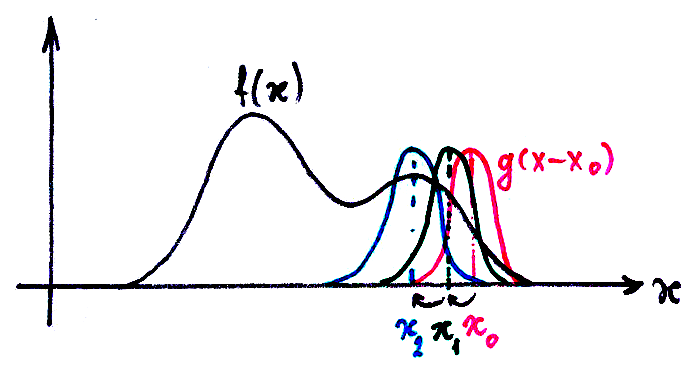
\includegraphics[width=0.8\linewidth]{metropolis.png}
    \caption{\label{dots-for-monte-carlo}Генерация последовательности случайных чисел в алгоритме
    Метрополиса.}
\end{figure}

Из теории цепей Маркова известно, что для того, чтобы распределение чисел цепи сходилось к
(существующему и единственному) распределению $f(x)$, достаточно выполнения
условия детального равновесия:
\begin{equation}
    \label{metropolis_detailed_balance}
    P(x' \to x) f(x') = P(x \to x') f(x),
\end{equation}
где $P(x_1 \to x_2)$ есть вероятность перехода в марковском процессе из точки $x_1$ в точку $x_2$.
Очевидно, что для алгоритма Метрополиса можно записать $P(x \to x') = g(x - x') \, A(x \to x')$, где
$A$ --- вероятность принятия, определяемая шагом~\ref{metropolis_acceptance} и, следовательно,
равная $A(x \to x') = \min \{1, f(x') / f(x) \}$. Подставляя $A$ и $P$ в
уравнение~(\ref{metropolis_detailed_balance}), легко убедиться, что оно выполнено.

Таким образом, суть алгоритма Метрополиса состоит в том, что мы заставляем некоторую точку блуждать
в пространстве случайным образом (но в то же время подчиняясь некоторому закону). При этом на
каждом шаге от своего текущего положения точка не может отойти дальше, чем <<ширина>> функции $g$.
Следовательно, если мы выберем $g$ много уже, чем характерная ширина функции $f$, то для того,
чтобы последовательность $x_i$ <<покрыла>> ширину функции $f$, потребуется очень много шагов. В то
же время, если мы выберем $g$ гораздо шире, чем $f$, то на большинстве шагов мы получим $x_{i + 1}
= x_i$. Таким образом, ширина распределения $g$ в оптимальном случае должна быть порядка ширины
функции $f$.

\textit{Вопрос.} Какой ширины должна быть proposal density в случае $f$, состоящей из двух пиков
шириной $a$ на расстоянии $b$ друг от друга? Эффективен ли алгоритм Метрополиса в данном случае?
Что произойдёт, если мы выберем $x_0$ вдали от пиков функции $f$?

\subsubsection{Метод имитации отжига}

\begin{figure}
	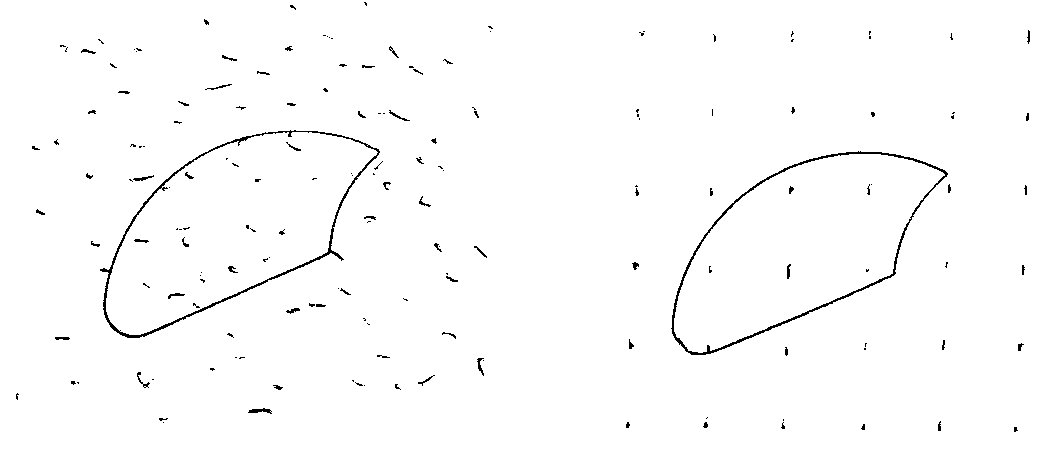
\includegraphics[width=1\linewidth]{dots-for-monte-carlo.png}
    \caption{\label{dots-for-monte-carlo}Заполнение фигуры случайными точками, имеющими равномерное
    распределение на плоскости (слева) и точками, находящимися в узлах регулярной прямоугольной
    сетки (справа).}
\end{figure}

\subsubsection{Вычисление интегралов методом Монте-Карло}

Как мы увидим, не всегда для вычисления интегралов достаточно использовать известный метод
прямоугольников или метод трапеций. И основная проблема здесь --- невысокая точность при вычислении
интегралов в пространстве высокой размерности. Например, попробуем оценить точность метода
прямоугольников при вычислении площади под прямой $y = x$ на отрезке $x \in [0, 1]$. Если для
вычисления мы возьмём $n$ прямоугольников, то ошибка вычисления интеграла, как легко вычислить,
будет порядка $O(1/n)$ ($n$ <<краешков>> прямоугольников площадью $\sim 1/n^2$ каждый попадают над
или под кривую, для которой мы вычисляем площадь). Если мы захотим вычислить методом
прямоугольников площадь под косо располозенной плоскостью, над основанием, разбитым на $n \times n$
прямоугольников (по осям $x$ и $y$), то ошибка снова будет порядка $O(1/n)$. Однако при этом
количество прямоугольников уже $\sim n^2$. Экстраполируя наши выводы на $D$-мерный интеграл, можно
заметить, что общее число прямоугольников ($\sim n^D$), и общее число вызовов интегрируемой
функции, растёт экспоненциально с ростом $D$ при сохранении определённого уровня точности ($\sim
1/n$). Это делает метод прямоугольников неприменимым в пространствах большой размерности. Наверное,
в этот момент стоит вспомнить, что в физике (и не только) встречаются задачи и в бесконечномерном
пространстве.

Метод Монте-Карло, который мы рассмотрим --- это настоящее математическое чудо, поскольку не
теребует экспоненциального роста числа точек в зависимости от размерности, при том, что он, на
первый взгляд, очень похож на метод прямоугольников. Суть простого (геометрического) метода
Монте-Карло состоит в следующем.  <<Накидываем>> (случайно! равномерно!) точки на плоскость, на
которой проведена кривая, площадь под которой мы хотим вычислить. Считаем те точки, что попали под
кривую. Отношение их к общему числу точек есть отношение площади области, в которой генерируем
точки, к площади под кривой. Если бы мы распределяли точки не случайным образом, а, скажем, ставили
бы их в узлах прямоугольной сетки (см. рисунок~\ref{dots-for-monte-carlo}), и использовали в методе
Монте-Карло, то получили бы те же проблемы, что и в методе прямоугольников.  <<Случайность>> точек
позволяет избавиться от этих проблем --- как мы покажем позже, ошибка метода Монте-Карло зависит то
количества точек, $N$, как $O(1/\sqrt{N})$. Стоит отметить, что в эту формулу размерность
пространства вообще никак не входит.  Таким образом, в среднем для уменьшения ошибки вдвое нам
нужно увеличить число точек в 4 раза, в то время как в случае использования метода прямоугольников
нам потребовалось бы вдвое увеличить разбиение по каждой оси, при этом общее число точек выросло бы
в $2^D$ раз.

\textit{Задача о вычислении объёма многомерного шара}. Требуется написать программу, вычисляющую с
помощью геометрического метода Монте-Карло объём $V$ шара единичного радиуса в пространстве
размерности $D$ и построить график $V(D)$ вплоть до $D = 10$. Можно заметить, что ошибка метода
(обозначим её $\varepsilon$), то есть разница вычисленного и реального объёмов, есть случайная
величина. Для $D = 2$ и $D = 3$ требуется построить зависимость среднеквадратичного отклонения
$\sigma$ для случайной величины $\varepsilon$ от числа точек, $N$, и показать, что
$\sigma_\varepsilon \sim 1 / \sqrt{N}$.

Есть не-геометрическая вариация метода Монте-Карло для вычисления интегралов, ещё больше похожая на
метод прямоугольников, но, тем не менее, обладающая той же точностью, что и геометрический метод. А
именно, интеграл от функции $f(x)$ вычисляется через сумму её значений в случайных точках, имеющих
равномерное распределение:
\begin{equation}
    \int_a^b f(x) \, dx \approx \frac{(b - a)}{N} \sum_{i=1}^N f(x_i).
\end{equation}
В методе прямоугольников используется та же формула, но точки распределены на отрезке $[a, b]$ с
постоянным шагом.

Интересно, что метод Монте-Карло в завуалированном виде встречается и в чистой математике. Так,
известный критерий Вейля говорит, что распределение чисел $x_j$ равномерно на $(0, 1)$ если и
только если для всех натуральных $\ell$ выполнено
\begin{equation}
    \lim_{N \to \infty} \frac{1}{N} \sum_{j = 1}^N \exp(2 \pi i \ell x_j) = 0.
\end{equation}
Видно, что этот критерий в определённом смысле эквивалентен утверждению, что <<интеграл от функции
$\sin x$ на её периоде равен нулю>>.

\clearpage

\section{Gradle, Lets-plot и Множество Жyлиа}

Возможно, читатель уже убедился на личном опыте, что скачивание и установка зависимостей вручную
--- не лучшая идея. Это не просто неудобно, но и может приводить к конфликтам версий библмотек и
различным ошибкам. Поэтому процесс сборки проекта и установки зависимостей давно пытаются
автоматизировать. Например, в Linux довольно часто используется GNU Make, отслеживающий, какие
файлы были изменены и что именно необходимо скомпилировать заново. Для упрощения работы с
зависимостями систему сборки объединяют с менеджером пакетов (Cargo в Rust, Haskell Stack, Nix). Мы
же рассмотрим Gradle --- систему сборки, которая широко используется для проектов на Kotlin и Java.

\begin{figure}
    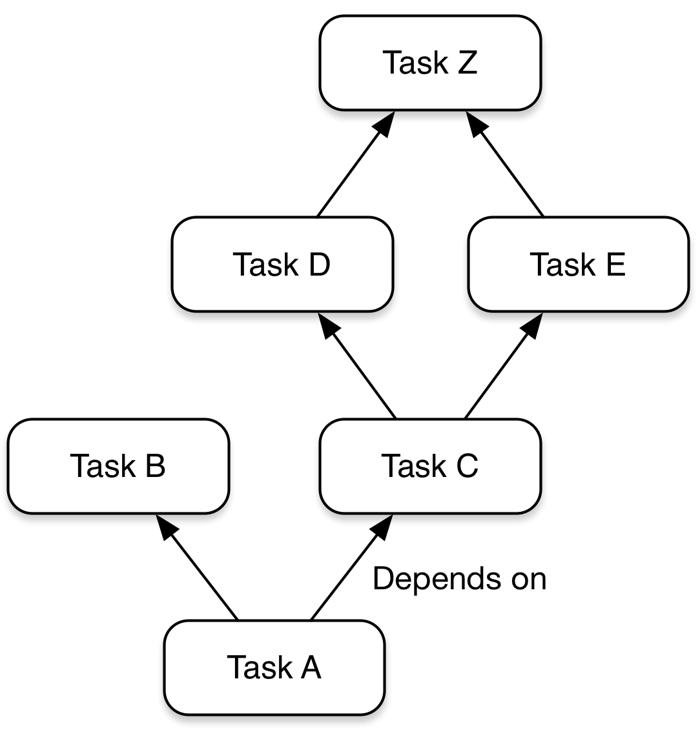
\includegraphics[width = 0.5\linewidth]{gradle_graph.png}
    \caption{\label{gradle_graph}Граф задач Gradle.}
\end{figure}

Конфигурация проекта в Gradle описывается как набор задач и связей (зависимостей) между ними
(рисунок~\ref{gradle_graph}). Задачей может быть как сборка проекта, так и запуск исполняемого
файла, сборка тестов и т. п. При этом сам проект может состоять из нескольких суб-проектов.
Название проекта и суб-проектов определяются в файле settings.gradle.kts, который в простейшем
случае содержит лишь имя проекта, например
\begin{minted}{kotlin}
rootProject.name = "lets-plot-gradle-example"
\end{minted}

Всё самое интересное (граф задач) описывается в файле build.gradle.kts, который сам по себе
является Kotlin-скриптом, использующим, на самом деле специально определённый для Gradle набор
функций и классов (Domain Specific Language, DSL). При этом стандартный задачи для компиляции и
запуска приложений, написанных на Kotlin, в Gradle уже описаны в соответствующем плагине.  Мы
рассмотрим простое приложение, которое при запуске рисует картинку с помощью библиотеки lets-plot.
Сама библиотека lets-plot разбита на части, мы воспользуемся двумя из таких частей. При этом
скачаем библиотеки из репозитория Maven Cental:
\begin{minted}{kotlin}
// файл build.gradle.kts

// Этот плагин добавляет поддержку Котлина
plugins {
    kotlin("jvm") version "1.4.32"
}

// версия нашего проекта
version = "1.1"

// Используем известный репозиторий Java-проектов,
// поддерживаемый Apache Software foundation
repositories {
    mavenCentral()
}

// библиотеки из Maven Central,
// функции из которых мы будем использовать в нашем коде
dependencies {
    implementation("org.jetbrains.lets-plot:lets-plot-kotlin-jvm:3.0.2")
    implementation("org.jetbrains.lets-plot:lets-plot-image-export:2.1.0")
}
\end{minted}
Сам проект можно найти по ссылке https://github.com/EvgenyNerush/lets-plot-gradle-example

\subsubsection{Lets-plot}

Lets-plot практически копирует пакет ggplot2, написанный на языке R. Его отличие от многих других
пакетов в том, что он не просто предоставляет набор функций для создания определённых типов
графиков, а предоставляет некоторую \textit{грамматику} для компоновки независимых компонентов,
благодаря чему легко создавать как новые типы графиков, так и компоновать графики друг с другом.

График в ggplot2 (и, соответственно, в Lets-plot) --- это набор данных, способ их отображения в
геометрические объекты (точки, линии) или ``эстетические'' аттрибуты (цвет, форма, размер, важно,
что они меняются в зависимости от данных), а также как минимум один \textit{слой} (layer),
представляющий всё вышеперечисленное. Слои обычно создаются с помощью
\mintinline{kotlin}{geom} функций. Подробное описание ggplot2 дано, например, в этой книге
https://ggplot2-book.org/index.html A мы рассмотрим пример:
\begin{minted}{kotlin}
// файл main.kt

import jetbrains.letsPlot.export.ggsave
import jetbrains.letsPlot.geom.geomLine
import jetbrains.letsPlot.geom.geomPoint
import jetbrains.letsPlot.geom.geomSmooth
import jetbrains.letsPlot.letsPlot

fun main() {
    // определяем "облако" из точек
    val xs = listOf(1, 2, 2, 3, 3, 3, 4, 5, 5, 5, 5)
    val ys = listOf(8, 7, 4, 5, 4, 3, 4, 3, 2, 1, 2)
    val zs = listOf(0, 0, 0, 0, 1, 0, 1, 1, 1, 1, 1)

    // готовим данные для letsPlot в виду key-value хранилища
    val data = mapOf<String, Any>("xvals" to xs, "yvals" to ys, "zvals" to zs)

    // график = данные + один слой + другой слой
    val fig_1 = letsPlot(data) +
            // здесь цвет - просто свойство точек
            geomPoint( color = "dark-green"
                     , size = 3.0
                     ) { x = "xvals"; y = "yvals" } +
            geomLine() { x = "xvals"; y = "yvals" }

    // сохраняем в файл
    ggsave(fig_1, "plot_1.png")

    // ещё график
    val fig_2 = letsPlot(data) +
            // а здесь цвет - эстетика, он зависит от данных
            geomPoint(size = 3.0) { x = "xvals"; y = "yvals"; color = "zvals"} +
            // рисует усреднённые данные и разброс
            geomSmooth() { x = "xvals"; y = "yvals"}

    ggsave(fig_2, "plot_2.png")

    println("bye!")
}
\end{minted}
Результатом работы этого кода являются рисунки~\ref{lets-plot-example-1}
и~\ref{lets-plot-example-2}

\begin{figure}
    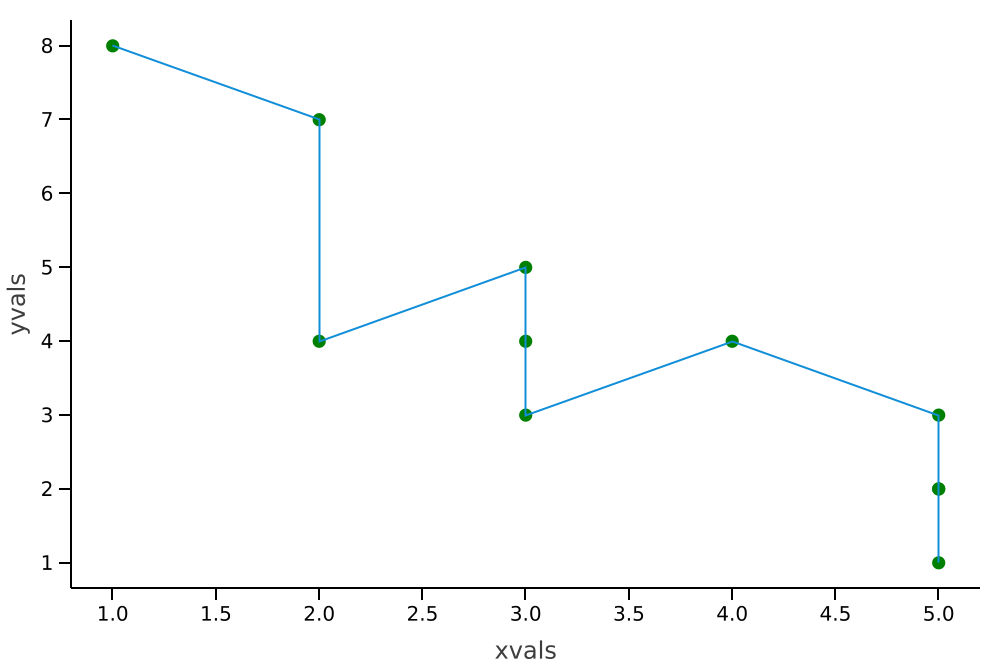
\includegraphics[width = 0.8\linewidth]{lets-plot-example-1.png}
    \caption{\label{lets-plot-example-1}Пример 1}
\end{figure}
\begin{figure}
    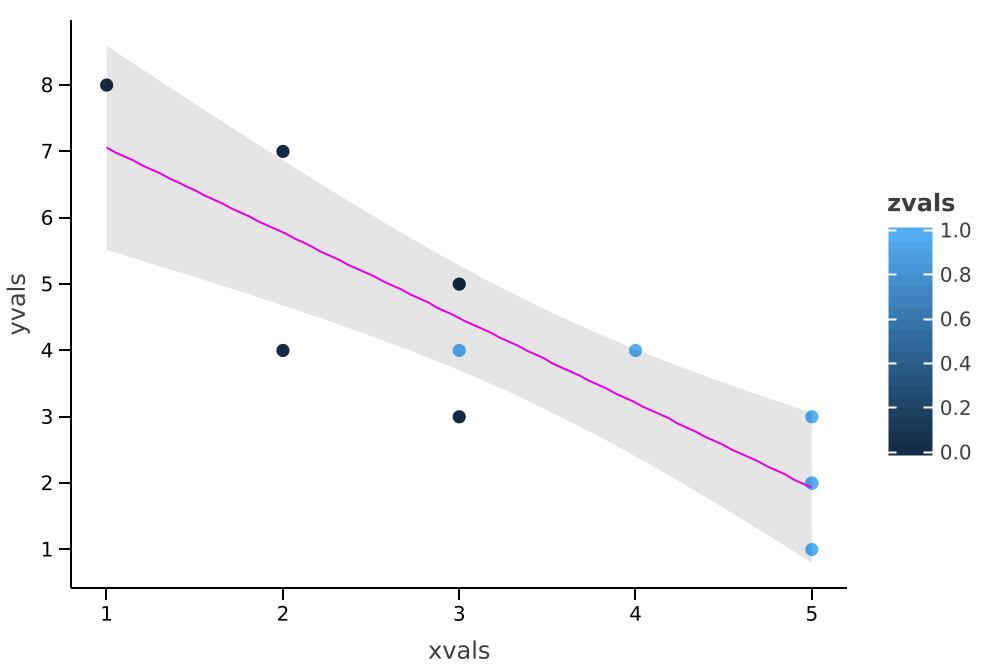
\includegraphics[width = 0.8\linewidth]{lets-plot-example-2.png}
    \caption{\label{lets-plot-example-2}Пример 2}
\end{figure}

\clearpage

\subsection{Множество Жулиа}

Есть комплексное отображение:
\begin{equation}
    f(z) = z^2 - 0.4 + 0.6 i,
\end{equation}
И есть последовательность
\begin{equation}
    g(n) = f^n = f(f( ...)(z), \; n \text{ раз}.
\end{equation}
Задача: построить распределение $n: \; \operatorname{abs}(g(n)(z)) <= 2$ в плоскости $z$ ($x \in [-2, 2]$, $y \in
[-2, 2]$. Можно взять $400 \times 300$ точек, $150$ итераций.  Дополнительные баллы за палитру,
красоту, подписи осей (tex) и т. п.. Делать - как минимум вдвоём.

\section{Доска Гальтона, задача о пьяном человеке и центральная предельная теорема}

\begin{figure}
    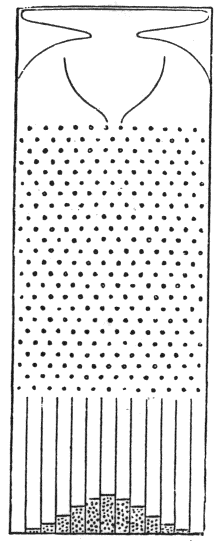
\includegraphics[width=0.7\linewidth]{Galton_board.png}
    \caption{\label{Galton_board}Устройство для демонстрации центральной предельной
    теоремы. Рисунок Гальтона, 1889 год.}
\end{figure}

В математике встречаются настоящие чудеса. Одно из самых известных - центральная предельная теорема
(ЦПТ). Мы увидим, что именно благодаря ей можно найти зависимость ошибки интегрирования методом
Монте-Карло от числа используемых точек и (главное!) показать, что эта зависимость никак не зависит
от размерности пространства. Однако начнём мы со связи центральной предельной теоремы и уравнений в
частных производных --- не столько для доказательства ЦПТ, сколько для демонстрации связи
совершенно разных разделов математики.

Фрэнсис Гальтон тоже был восхищён центральной предельной теоремой, и для её демонстрации в 1873
году изобрёл специальное устройство (рисунок~\ref{Galton_board}), позже названное в его честь (в
английской литературе помимо Galton board используется bean machine). Устройство состоит из
регулярных рядов гвоздиков, поперёк которых из одной и той же точки насыпаются мелкие шарики
(зёрнышки, дробинки и т. п.), которые после прохождения рядов гвоздиков собираются в корзинки
(bins). Таким образом, высота столбиков, образованных зёрнышками в корзинках, демонстрирует функцию
распределения зёрнышек.

Как распределены зёрнышки по корзинкам? Чтобы ответить на этот вопрос, построим простейшую
математическую модель доски Гальтона. В доске Гальтона зёрнышки отскакивают от гвоздиков в
случайном направлении и на достаточно случайное расстояние. Мы же будем рассматривать одиночное
зёрнышко, которое на каждой итерации будет перемещаться вдоль оси $x$ на расстояние, равное $+1$
или $-1$ с равной вероятностью. Зададимся вопросом, какова вероятность найти зёрнышко с координатой
$j$ после $i$ итераций?  Данная математическая модель по понятным причинам носит название
<<задача о пьяном человеке>>.  Внимательный читатель заметит, что если при $i = 0$ зёрнышко
находилось в точке $j = 0$, то далее при нечётных значениях $i$ оно всегда будет иметь нечётную
координату $j$, а при чётных --- чётную.  Для того, чтобы <<сгладить>> распределение зёрнышек,
будем считать, что изначатьно при $i = 0$ зёрнышко стартует с $j = 0$ или с $j = 1$, с вероятностью
$1/2$ каждая.


Введём обозначение $P(i, j)$ --- вероятность того, что после $i$ итераций зёрнышко окажется в точке с
координатой $j$. Тогда можно записать связь распределения вероятности зёрнышек для $i$ и $i+1$
итераций:
\begin{equation}
    \label{P_drunk_man}
    P(i+1, j) = \frac{1}{2} P(i, j - 1) + \frac{1}{2} P(i, j + 1)
\end{equation}
(с вероятностью $1/2$ зёрнышко с координатой $j - 1$ пойдёт вправо, и с вероятностью $1/2$ зёрнышко
с координатой $j + 1$ пойдёт влево).
Можно заметить, что при большом числе итераций ($i \gg 1$) характерная ширина
функции $P(i, j)$ по координате $j$ (то есть характерная ширина распределения зёрнышек в доске
Гальтона) много больше единицы. При этом уравнение~(\ref{P_drunk_man}) можно записать в виде
\begin{equation}
    P(i+1, j) - P(i, j) = \frac{P(i, j + 1) - 2 P(i, j) + P(i, j - 1)}{2}.
\end{equation}
и рассматривать как численную аппроксимацию уравнения в частных производных:
\begin{equation}
    \label{heat_equation}
    \frac{\partial P}{\partial t} = \frac{1}{2} \frac{\partial^2 P}{\partial x^2},
\end{equation}
где вместо дискретных $i$ и $j$ введены, соответственно, непрерывные $t$ и $x$.

Уравнение~(\ref{heat_equation}) носит название уравнения теплопроводности (поскольку, в том числе,
описывает распространение тепла). С помощью подстановки легко проверить, что это уравнение имеет
следующее частное решение:
\begin{equation}
    P(t, x) = \frac{1}{s} e^{-\frac{x^2}{2 s^2}}, \qquad s(t) = \sqrt{t}.
\end{equation}
\textit{Вопрос}. Проверить, что данная функция является решением уравнения теплопроводности.

Заменяя в этом решении $x$ на $j$ и $t$ на $i$, получим приближённое решение задачи о пьяном человеке. Таким
образом, мы видим, что совершенно стохастический процесс иногда может быть описан с помощью
дифференциального уравнения. Позже мы увидим обратный пример, где для решения дифференциального
уравнения нам придётся построить определённый стохастический процесс.

Какое отношение наша математическая модель имеет к реальной доске Гальтона? Как полученное решение
будет зависеть от функции, описывающей рассеяние зёрнышка на отдельном гвоздике? Чтобы ответить на
этот вопрос, усложним нашу задачу --- введём функцию рассеяния $w_k$ --- вероятность того, что
зёрнышко отскочит на расстояние $k$ от текущего гвоздика. Очевидно, $\sum_k w_k = 1$. С введением
функции рассеяния соотношение~(\ref{P_drunk_man}) заменится следующим:
\begin{equation}
    \label{advanced_drunk_man}
    P(i+1, j) = \sum_k w_k P(i, j - k).
\end{equation}
Аналогично тому, как мы это делали ранее, мы можем считать, что функция $P(i, j)$ --- плавная по
обеим координатам, и использовать непрерывные координаты $t$ и $x$ вместо дискретных $i$ и $j$.
Тогда, заменяя конечные разности производными, получим:
\begin{multline}
    P(i + 1, j) - P(i, j) = \sum_k w_k P(i, j - k) - P(i, j) \sum_k w_k \\
    = \sum_k w_k \left[ P(i, j - k) - P(i, j) \right] \approx - \sum_k w_k k \left( \frac{\partial
    P}{\partial x} \right)_{j - k/2}.
\end{multline}
В последнем слагаемом индекс обозначает точку по $x$, в которой берётся производная от $P$.
Несмотря на то, что функция $P$ плавная, мы не можем вынести $\partial P / \partial x$ за знак
суммы, поскольку $k$ в сумме может быть как положительным, так и отрицательным и, вынося
производную за знак суммы, мы можем потерять ведущее слагаемое в нашем уравнении (а в
случае симметричной функции рассеяния $\sum_k w_k k = 0$, и мы просто получим ноль в правой части).
Казалось бы, мы можем переписать наше уравнение так:
\begin{multline}
    \label{P_error}
    P(i + 1, j) - P(i, j) = -\left( \frac{\partial P}{\partial x} \right)_j \sum_k w_k k \\
    + \sum_k w_k k \left[ \left( \frac{\partial P}{\partial x} \right)_j - \left( \frac{\partial
    P}{\partial x} \right)_{j - k/2} \right] \\
    \approx - \left( \frac{\partial P}{\partial x} \right)_j \sum_k w_k k + \sum_k \frac{w_k
    k^2}{2} \left( \frac{\partial^2 P}{\partial x^2} \right)_{j - k/4}.
\end{multline}
Однако и здесь нельзя выносить (теперь уже вторую) производную за знак суммы! Для того, чтобы это
понять, рассмотрим следующий пример.

Пусть $w_k = 1$ для $k = 1$ и $w_k = 0$ для всех прочих $k$. Тогда, очевидно, такая доска Гальтона
на каждом шаге будет просто смещать зёрнышки вправо, а эволюция функции распределения будет
описываться переносом, $P(t, x) = P(0, x - t)$. Дифференциальное уравнение, описывающее перенос,
есть $\partial P / \partial t = -\partial P / \partial x$, и оно не содержит второй производной.
Однако для выбранной функции рассеяния $\sum w_k k^2 = 1$, и вторая производная (которой не должно
быть) возникает в уравнении~\ref{P_error}. Это говорит об ошибочности подхода с выносом второй
производной из суммы.

Можно догадаться, что избавиться от зависимости производных от $k$ возможно, вычисляя производные
$\partial P / \partial x$ в той точке, из которой происходит перенос функции $P$, а именно в точке
$j - \mu$, где
\begin{equation}
    \mu = \sum_k w_k k.
\end{equation}
Учитывая, что $j - k = j - \mu + (\mu - k)$, меем:
\begin{equation}
    P(i, j - k) \approx P(i, j - \mu) + \left( \frac{\partial P}{\partial x} \right)_{j - \mu} (\mu
    - k) + \left( \frac{\partial^2 P}{\partial x^2} \right)_{j - \mu} \frac{(\mu - k)^2}{2}.
\end{equation}
Тогда из~\ref{advanced_drunk_man} получаем:
\begin{multline}
    P(i + 1, j) - P(i, j) = \sum_k w_k \left[ P(i, j - \mu) - P(i, j) \right. \\
    \left. + \left( \frac{\partial P}{\partial x} \right)_{j - \mu} (\mu - k) + \left(
    \frac{\partial^2 P}{\partial x^2} \right)_{j - \mu} \frac{(\mu - k)^2}{2} \right] \\
    \approx -\mu \left( \frac{\partial P}{\partial x} \right)_{j - \mu/2} + \frac{1}{2} \left(
    \frac{\partial^2 P}{\partial x^2} \right)_{j - \mu} \sum (k - \mu)^2 w_k,
\end{multline}
здесь мы воспользовались соотношением $\sum (\mu - k) w_k = 0$, а также тем, что производные уже не
зависят от $k$, что позволило вынести их за знак суммирования. Очень важно, чтобы и первая, и
вторая производные брались в одной и той же точке. Здесь же они берутся в разных точках, поэтому
нужно быть осторожным:
при изменении точки, в которой берётся первая
производная, возникает дополнительное слагаемое со второй производной. Однако можно заменить во
втором слагаемом (без потери точности) точку взятия производной на $j - \mu/2$. Производную по
времени также можно рассматривать в этой точке (что не вполне корректно?). В итоге, приходим к
следующему дифференциальному уравнению:
\begin{equation}
    \label{heat_equation_mu_sigma}
    \frac{\partial P}{\partial t} = -\mu \frac{\partial P}{\partial x} + \frac{\sigma^2}{2}
    \frac{\partial^2 P}{\partial x^2}, \qquad \mu = \sum_k w_k k, \qquad \sigma^2 = \sum_k  (k -
    \mu)^2 w_k.
\end{equation}

\textit{Вопрос}. Покажите, что замена переменных $t = t'$, $x = \sigma x' + \mu t'$ переводит это
уравнение к виду уравнения теплопроводности~(\ref{heat_equation}) в координатах $t'$ и $x'$.

\textit{Вопрос}. Вычислите $\mu$ и $\sigma$ для модельной задачи о пьяном человеке ($w_k = \pm 1/2$
для $k = \pm 1$).

Решение уравнения~(\ref{heat_equation_mu_sigma}), аналогичное приведённому выше частному решению
уравнения теплопроводности, имеет следующий вид:
\begin{equation}
    \label{heat_equation_mu_sigma_solution}
    P(t, x) = \frac{1}{s'} \exp \left[-\frac{(x - \mu t)^2}{2 s'^2} \right], \qquad s'(t) = \sigma
    \sqrt{t}.
\end{equation}
Что значит это решение с точки зрения задачи о доске Гальтона? Во-первых, видно, что в случае
несимметричной функции рассеяния возникает снос <<колокольчика>> со скоростью $\mu$. Во-вторых,
ширина распределения зёрнышек, как и прежде, растёт пропорционально $\sqrt{t}$.
Но самое главное --- то, что детальный вид функции $w_k$ для поведения решения не важен --- важны
только первые её два момента, $\mu$ и $\sigma$! На самом деле это далеко не очевидный результат.

В задаче о доске Гальтона положение зёрнышка есть сумма случайных смещений, которые придают ему
ряды гвоздиков. Из полученного решения следует, что среднее положение зёрнышек после $i$ отскоков
есть $\mu i$, а среднеквадратичное отклонение случайной величины --- положения зёрнышка ---
есть $s' = \sigma \sqrt{i}$.

\textbf{Центральная предельная теорема} рассматривает ситуацию, очень похожую на задачу о доске
Гальтона. А именно, пусть случайная величина $x$ есть сумма (независимых!) случайных величин $x_i$,
которые соизмеримы (то есть, грубо говоря, их средние $\mu_i$ одного порядка, и их дисперсии
$\sigma_i^2$ одного порядка). Для доски Гальтона, как уже было сказано, смещение равнялось сумме
случайных величин --- смещений, имеющих одно и то же распределение. Так вот, ЦПТ утверждает, что при $i \gg 1$
среднее $\mu$ и дисперсия $\sigma^2$ случайной величины $x$ есть сумма средних и дисперсий,
соответственно, для величин $x_i$,
\begin{equation}
    \mu = \sum_i \mu_i, \qquad \sigma^2 = \sum_i \sigma_i^2,
\end{equation}
а распределение $x$ имеет гауссов вид, аналогичный~(\ref{heat_equation_mu_sigma_solution}). На
практике оказывается, что часто даже для двух-трёх случайных величин распределение их суммы очень
похоже не гауссово. Чтобы <<прочувствовать>> ЦПТ, попробуйте ответить на несколько вопросов.

\textit{Вопрос}. Найдите среднее и дисперсию распределения зёрнышек по корзинкам для доски
Гальтона, пользуясь ЦПТ.

\textit{Вопрос}. Придумайте контрпримеры для ЦПТ, нарушая то или иное её условие. Например, в
алгоритме Метрополиса текущее состояние цепи Маркова есть сумма смещений из её предыдущих
состояний. Почему, тем не менее, алгоритм Метрополиса генерирует распределение, не подчиняющееся
ЦПТ?

\textit{Вопрос}. Рассмотрите случайную величину $N_{in}$ --- число точек, попавших внутрь фигуры,
площадь которой мы пытаемся найти, производя интегрирование методом Монте-Карло. Чему равно среднее
и дисперсия этой случайной величины, как она зависит от общего числа точек $N$? Как ошибка
интегрирования метода Монте-Карло зависит от $N$ и от размерности пространства?

\section{Функциональное программирование}

Императивное (команды), ОО (инкапсуляция, наследование) и функциональное (декларация, описание)
программирование.

Каким должен быть научный код? Он должен быть открытым, но и рецензируемым в первую очередь. Это
значит, что он должен быть не только читаемым и понятным, хорошо документированным, но и
тестируемым.  Главным здесь (как и для ненаучного кода) становится модульность. Аналогия со
структурным программированием. Код - совокупность и последовательное применение функций.
Функциональное программирование. Переиспользование кода (функций). Это ещё и ключ к простоте кода.

Why functional programming matters? John Hughes, 1990. Рассмотрим кусочек этой работы. Код в той
работе - на Miranda, здесь же мы попробуем убить двух зайцев --- разобраться с классической работой
и понять, как использовать функциональную парадигму в Kotlin.

Функция высшего порядка --- функция, принимающая и (или) возвращающая другую функцию.

\begin{minted}{kotlin}
    //// Functions are the first-class passengers ////

    // any function of Pi; note functional type here
    fun ofPi(f: (Double) -> Double): Double {
        return f(PI)
    }

    val r = ofPi(::sin) // note `::`
    println("$r") // 1.2e-16

    // Composition of functions, f.g: (f.g)(x) = f(g(x))
    // note a closure (lambda function)
    fun <A, B, C> compose(f: (B) -> C, g: (A) -> B): (A) -> C =
        { x -> f(g(x)) }

    // `n` times apply `f`;
    // Recursion instead of a loop;
    // Without `x`, just functions and composition
    fun apply(f: (Double) -> Double, n: Int): (Double) -> Double =
        if (n == 1) f else compose(apply(f, n - 1), f)

    // let's try
    fun g(x: Double) = x * x
    val h = apply(::g, 2) // (x^2)^2 = x^4
    println("${h(2.0)}") // 16.0
\end{minted}

Алгебраический тип данных - составной тип, представляющий собой тип-сумму из типов-произведений.
Тип-сумма - объединение типов (как алфавит - объединение букв). Тип-произведение - декартово
произведение (кортеж, пара координат, например). Список, дерево - алгебраические типы данных?

\begin{minted}{kotlin}
// just an example of a class
class MyPair(i: Int, j: Int) { /*...*/ }

// `object` keyword creates a type with only one instance, i.e. a singleton
object MyUselessSingleton { /* something can be here */ }

// Algebraic data types: an example;
// `sealed` ~ not extendable
sealed class Maybe {
    // singleton `None` inheriting `Maybe`
    object None : Maybe()
    // data class holds data only
    data class Just(val value: Double) : Maybe()
}
\end{minted}

Теперь попробуем их использовать.

\begin{minted}{kotlin}
    fun printJust(x: Maybe) {
        // pattern matching
        when (x) {
            is Maybe.Just -> println("${x.value}")
            is Maybe.None -> println("None")
        }
    }

    val num = Maybe.Just(5.0)
    printJust(num) // 5.0
\end{minted}

Список. Kotlin: Any, Unit and Nothing.
\begin{minted}{kotlin}
// list as a recursive class: it is either an empty list
// or a value (head) attached to another list;
// Note `out` and `Nothing` (type with no instance) here
sealed class MyList<out T> {
    object Nil : MyList<Nothing>() // object can't have a generic type in Kotlin
    data class Cons<T>(val head: T, val tail: MyList<T>) : MyList<T>()
}
\end{minted}

Использование.
\begin{minted}{kotlin}
    /* "Modular design brings with it great productivity improvements.
   First of all, small modules can be coded quickly and easily. Second,
   general-purpose modules can be reused, leading to faster development
   of subsequent programs. Third, the modules of a program can be tested
   independently, helping to reduce the time spent debugging."
   John Hughes, "Why Functional Programming Matters", 1990
    */

    // []
    val a = MyList.Nil
    // [1]
    val b = MyList.Cons(1, MyList.Nil)
    // [1, 2]
    val c = MyList.Cons(1, MyList.Cons(2, MyList.Nil))

    fun sum(list: MyList<Int>): Int {
        val res = when (list) {
            is MyList.Nil  -> 0
            is MyList.Cons -> list.head + sum(list.tail)
        }
        return res
    }

    println("sum([1,2]) = ${sum(c)}") // 3
\end{minted}

Как эту функцию разбить на части? Как можно обобщить такую простую функцию?
\begin{minted}{kotlin}
    /* Only `0` and `+` in the definition of `sum` are specific to computing a sum.
    This means that the computation of a sum can be modularized by gluing together
    a general recursive pattern with `0` and `+`. This recursive pattern is
    conventionally called `foldr` (right fold).
     */
    fun <A, B> foldr(plus: (A, B) -> B, zero: B, list: MyList<A>): B {
        val res = when (list) {
            is MyList.Nil  -> zero
            is MyList.Cons -> plus(list.head, foldr(plus, zero, list.tail))
        }
        return res
    }

    fun newSum(xs: MyList<Int>) = foldr(Int::plus,0, xs)
    println("newSum([1,2]) = ${newSum(c)}") // 3

    /* And now `foldr` can be reused! */

    // note zero = 1 here
    fun product(xs: MyList<Int>) = foldr(Int::times,1, xs)
    fun anyTrue(xs: MyList<Boolean>) = foldr( Boolean::or, false, xs)
    fun allTrue(xs: MyList<Boolean>) = foldr( Boolean::and, true , xs)

    // [4, 1, 2]
    val ints = MyList.Cons(4, c)
    println("product([4,1,2]) = ${product(ints)}") // 8
    // [false, true]
    val bools = MyList.Cons(false, MyList.Cons(true, MyList.Nil))
    println("anyTrue([0,1]) = ${anyTrue(bools)}") // true
    println("allTrue([0,1]) = ${allTrue(bools)}") // false
\end{minted}

Можно заметить, что...
\begin{minted}{kotlin}
    /* "One way to understand `foldr` is as a function that replaces all occurrences
    of `Cons` in a list by `plus`, and all occurrences of `Nil` by `zero`."
    Cons(1, Cons(2, Nil))
    plus(1, plus(2,   0))
     */

    // Thus foldr(Cons, Nil, xs) = xs, and we can reuse `foldr` even further,
    // e.g. we can substitute `Nil` with another list:

    // I don't know how to pass `Cons()` directly to `append`
    fun <T> cons(x: T, xs: MyList<T>): MyList.Cons<T> {
        return MyList.Cons(x, xs)
    }
    fun <T> append(xs: MyList<T>, ys: MyList<T>): MyList<T> = foldr(::cons, ys, xs)
    println("sum [4,1,2,4,1,2] = ${sum(append(ints, ints))}") // 14

    // That if we substitute `Cons()` with `count`?
    fun <T> count(x: T, n: Int): Int = n + 1
    // `count` increments 0 as many times as there are `Cons`
    fun <T> length(xs: MyList<T>): Int = foldr(::count, 0, xs)
    println("length of [4,1,2] = ${length(ints)}") // 3

    // Now we would write a function which `plusOne` all the elements of a list,
    // for which we replace `Cons(x, xs)` with `Cons(plusOne x, xs)`. However, this can be
    // generalized.
    fun <A, B> fandCons(f: (A) -> B): (A, MyList<B>) -> MyList<B> =
        { x, xs -> MyList.Cons(f(x), xs) }
    fun <A, B> map(f: (A) -> B, xs: MyList<A>): MyList<B> =
        foldr(fandCons(f), MyList.Nil, xs)
    // note that `map` can be obviously written using `when`

    fun plusOne(x: Int) = x + 1
    println("sum of [5,2,3] = ${sum(map(::plusOne, ints))}") // 10
\end{minted}

Функции map и foldr --- очень часто встречаются и в других языках. Как написать map для списков в
C++? Теория категорий.

\section{ЦПТ - повторение}

Шумы на фото.

\textit{Вопрос}. Рассмотрите случайную величину $N_{in}$ --- число точек, попавших внутрь фигуры,
площадь которой мы пытаемся найти, производя интегрирование методом Монте-Карло. Чему равно среднее
и дисперсия этой случайной величины, как она зависит от общего числа точек $N$? Как ошибка
интегрирования метода Монте-Карло зависит от $N$ и от размерности пространства?

\textit{Вопрос}. Для интегрируемой функции $f$ найдите (с точностью до постоянного множителя) свёртку
\begin{equation}
    g(x) = \int_{x - 1/2}^{x + 1/2} \int_{x_1 - 1/2}^{x_1 + 1/2} ... \int_{x_{n - 1} -
    1/2}^{x_{n - 1} + 1/2}
    f(x_n) \, dx_n \,
    ... \, dx_2 \, dx_1,
\end{equation}
где интегрирование производится $n$ раз, $n \gg 1$. Тоже для
\begin{multline}
    g(x) = \int_{-\infty}^\infty \int_{-\infty}^\infty ... \int_{-\infty}^\infty
    f(x_n) \exp\left[-(x_n - x_{n - 1})^2 \right] ...\\
    \exp\left[-(x_2 - x_1)^2 \right]
    \exp\left[-(x_1 - x)^2 \right]
    \, dx_n \, ... \, dx_2 \, dx_1,
\end{multline}
где интегрирование производится $n$ раз, $n \gg 1$.

\textit{Задача о вычислении объёма многомерного шара}. Требуется написать программу, вычисляющую с
помощью геометрического метода Монте-Карло объём $V$ шара единичного радиуса в пространстве
размерности $D$ и построить график $V(D)$ вплоть до $D = 10$. Можно заметить, что ошибка метода
(обозначим её $\varepsilon$), то есть разница вычисленного и реального объёмов, есть случайная
величина. Для $D = 2$ или $D = 3$ требуется построить зависимость среднеквадратичного отклонения
$\sigma$ для случайной величины $\varepsilon$ от числа точек, $N$, и показать, что
$\sigma_\varepsilon \sim 1 / \sqrt{N}$. Команда - 4 человека. Модульность, git (github.com),
параллельная версия - приветствуются.

\section{Уравнение Шредингера}

Какое отношение доска Гальтона имеет к квантовой механике? Мы рассмотрим задачу, упрощённо
представляющую симуляции, возникающие в калибровочных теориях на решётках (lattice gauge theory) ---
численном описании задач квантовой теории поля с сильной связью (квантовая хромодинамика, кварки,
глюоны...), где теория возмущений (которая используется в квантовой электродинамике) не работает.
Значительный вклад в lattice gauge theory внёс Кеннет Уильсон (Kenneth Wilson), лауреат Нобелевской
премии по физике 1982 года (``за теорию критических явлений в связи с фазовыми переходами'').

Что изменится, если зёрнышки с некоторой вероятностью $u(j)$ будут пропадать на гвоздиках? (Условно
можно сказать, что к доске Гальтона приделали пылесос).  Легко показать, что уравнение на функцию
распределения примет вид
\begin{equation}
    P(i+1, j) = [1 - u(j)]\sum_k w_k P(i, j - k).
\end{equation}
Домножая это уравнение на $[1 - u]^{-1}$ и вычитая $P(i,j)$, в правой части можно прийти к тем же
выражениям, что и ранее, в левой же части приближенно получится $\partial P / \partial t + u(j)
P(i, j)$.
Для простоты, мы выбрали $w_{-1} = w_1 = w_0 = 1/3$ ($\mu = 0$, $\sigma^2 = 2/3$) и 
$u(x) = \alpha x^2$, где $\alpha$ --- некоторый коэффициент. Тогда
\begin{equation}
    \label{Feynman_board}
    \frac{\partial P}{\partial t} = \frac{1}{3} \frac{\partial^2 P}{\partial x^2} - \alpha
    x^2 P.
\end{equation}
Это уравнение есть уравнение Шредингера в комплексном времени. Для того, чтобы перейти от него к
привычному виду уравнения Шредингера, сделаем замену 
$\tau
= i t$ при условии $\hbar / 2 m = 1 / 3$, $k / 2 \hbar = \alpha$,
которая даст
\begin{equation}
    \label{Schroedinger_oscillator}
    i \hbar \frac{\partial P}{\partial \tau} = - \frac{\hbar^2}{2 m} \frac{\partial^2
    P}{\partial x^2} + V(x) P,
\end{equation}
где $V(x) = k x^2 / 2$ --- потенциал, в котором находится частица, $k$ --- жесткость пружины.
Уравнение Шредингера~\ref{Schroedinger_oscillator} описывает поведение \textit{волновой функции}
гармонического осциллятора. Правая часть уравнения Шредингера есть применение оператора энергии к
функции $P$. Если мы найдём какую-либо собственную функцию оператора энергии $P_n(x)$ (соответствующему
собственному значению $E_n$ (то есть для неё $\hat H P_n = E_n P_n$), то ей будет соответствовать
решение уравнения Шредингера $P_n(x) \exp(-i E_n \tau / \hbar)$. При переходе к переменной $t$ из
этой зависимости от времени мы
получим убывающую экспоненту $\exp(- E_n t)$, а зависимость от $x$ останется прежней.

Предположим, что мы не можем по каким-то причинам решать напрямую уравнение Шредингера (например,
конечно-разностными методами), но хотим найти уровни энергии (хотя бы самые нижние). Тогда можно
попробовать, моделируя <<доску Гальтона с пылесосом>>, найти форму $P(x)$ для нижнего уровня и $E_0$,
подождав достаточно долго. Нижний уровень соответствует минимальной энергии, соответствующая
экспонента затухает медленнее всех, следовательно, только решение, соответствующее нижнему уровню,
выживет на больших временах.

\textit{Задача}
Из квантовой механики известно, что $E_n = \{\hbar \Omega / 2, 3 \hbar \Omega / 2, 5 \hbar \Omega /
2, ...\}$, где $\Omega = \sqrt{k / m}$ --- частота осциллятора в классической задаче. Смоделировать
<<доску Гальтона с пылесосом>> [для этого удобно ввести вес частиц, и вместо <<выкидывания>> частиц
уменьшать их вес на каждом шаге, в соответствии с $u(x)$], и найти $P(t, x)$ для некоторого
начального условия.  Используя найденную функцию, попытаться найти два-три нижних уровня энергии
($E_n$) и соответствующие собственные функции [стоит учесть, что любое решение уравнения Шредингера
представимо в виде суперпозиции собственных функций; уровни энергии удобно вычислять по наклону в
логарифмическом масштабе]. Для описанной выше доски Гальтона $Omega = 4 \alpha / 3$, что для
$\alpha = 10^{-4}$ даст $\Omega \approx 0.012$ (?!).

\section{Интегралы по траекториям}

Путешествую по доске Гальтона, разные зёрнышки проходят по разным траекториям. И можно задаться
вопросом, какова вероятность того, что зёрнышко выберет ту или иную траекторию. Зная вероятность
рассеяния и исчезновения зёрнышка $w_k$ и $u(j)$ можно найти вероятность конкретной траектории как
произведение ...

\subsection{Terminal. Git. IntelliJ tips and tricks.}

terminal idea project
\begin{minted}{bash}
help
help cd
cd
cd src\main
cd ..\..
help xcopy
xcopy /P src\main\kotlin\main.kt .
use tab, up arrow
dir
more main.kt
where /?
where /R . main.kt
del main.kt
ping 8.8.8.8
ping ya.ru
exit
\end{minted}

Git --- система контроля версий (ещё есть SVN, Mercurial...), позволяет хранить различные версии
кода, просматривать разницу между ними, а также чрезвычайно удобна для совместной разработки.
Хранит изменения, а не весь код. При таком подходе, если разные люди работают над разными частями
кода, их изменения можно легко соединить (merge). Ветки. git status, log, commit, pull, push.

VCS/Import into version control/Create GIT repository...
Cannot run git, download...
all default...

Git GUI
New - dir of project, close. git bash, ls -la
intellij, перезапустить idea, пкм main.kt (слева), git add, внизу - version control, commit, log
hello, universe - посмотреть изменения в окне version control

version control, local changes.
println("qwe"), разицу видно в реальном времени

в консоли проекта:
git status
modified: src/main...main.kt
git add main.kt
git status // modified - зеленым
git commit -m 'Universe instead of world'
git status .. nothing to commit
git log

git pull
git push
git branch
git checkout

tips, rename fun and alt +enter, ctrl y, ctrl w, x.for enter, x.if enter, drag and dock tabs, git
diff, comput with shift shift, extract parameter ctrl alt p, select all occurences ctrl alt shift
j, ctrl shift f12, code completeon ctrl shift enter or space, ctrl shift t, help/learn ide
features, completeon with short names, alt ->, ctrl tab, ctrl e, ctrl shift e, ctrl shift v my
friend! alt enter driven development, ctrl shift m для навигации {}, ctrl alt t editor fold

слепая печать

\subsection{Функциональное программирование на практике}

\clearpage

\textit{Задача}. Cгенерировать массив псевдослучайных чисел с функцией распределения
\begin{equation}
    \frac{dN}{dx} \propto \exp(\sin(\pi x^2)), \qquad x \in (0, 1).
\end{equation}
Продемонстрировать корректность работы генератора:
\begin{enumerate}
  \item Найти функцию распределания полученного генератора, <<раскидав>> сгенерированные числа по
      корзинкам, и сравнив с теорией на графике.
  \item Найти и вывести на экран <<центр масс>> полученного распределения (среднее значение $x$).
        % 0.561418
  %\item для массива случайных точек из 10000 элементов измерить время генерации
  %    и нахождение среднего (суммарное), вывести на экран % 1 б за время, 1б за
  %    %хорошую скорость
  %      наперёд заданной длины (!)
\end{enumerate}

\clearpage

сначала плоская (альтернативный метод), потом любая p.

Пусть целевое распределение пропорционально функции $f(x)$, а шаги генерируются с распределением
$g(x - y)$, где $x$ --- текущая точка, $y$ --- следующая. Тогда на каждой итерации алгоритм
выглядит так:
\begin{enumerate}
    \item qwe
    \item qwz
\end{enumerate}

Интегрирование для неравномерного распределения. Пусть нам нужно вычислить интеграл от
произведения, $a(x) p(x)$:
\begin{equation}
    \int_a^b a(x) p(x) \, dx \approx \frac{\sum_{i=1}^N f(x_i)}{N},
\end{equation}
где $p$ --- плотность вероятности используемого случайного распределения, для равномерного
распределения --- константа. Если нужно вычислить интеграл от $f$ (для узкой $f$, например), то
можно сгенерировать распределение с плотностью вероятности $f$. Такой метод даст
меньшую ошибку.

Вильсон (не тот, что камера Вильсона). Интегралы по траекториям.

\subsection{Задача о пьяном человеке, доска Гальтона и Центральная предельная теорема}

Синяя тетрадь, оранжевые наклейки.

\subsection{Дз --- несимметричная доска Гальтона + решение уравнения Шредингера (нахождение уровней
энергии нижних трёх состояний, формы волновых функций? Найти $\Omega$ для $\alpha = 10^{-4}$,
должно получиться около $0.012$.}

Как ошибка в Монте-Карло интегрировании зависит от числа точек --- теперь можем ответить.
Рассмотрим геометрический метод Монте-Карло. Очевидно, что при фиксированном общем числе точек
число точек "под кривой" есть сумма большого числа случайных величин ($\pm 1$ с некоторой вероятностью, что
соответствует попаданию или непопаданию под кривую). Применив ЦПТ, получим, что число точек внутри
стремится к вероятности попасть под кривую, умноженной на общее число точек (закон больших чисел), а квадрат
среднеквадратичного отклонения (дисперсия) растет пропорционально числу частиц. Ошибка
интегрирования, равная среднеквадратичному отклонению, деленному на число точек $N$,
пропорциональна $1 / \sqrt{N}$.

На прошлой лекции --- уравнение теплопроводности. Для $w_{-1} = w_1 = 1/2$:
\begin{equation}
    \frac{\partial P}{\partial t} = \frac{1}{2} \frac{\partial^2 P}{\partial x^2},
\end{equation}
для произвольной $w$ вместо $1/2$ будет стоять $\sum_l l^2 w_l / 2$, что в случае $w_{-1} = w_1 =
w_0 = 1/3$ даст $1/3$. Сравним с уравнением Шредингера для гармонического осциллятора:
\begin{equation}
    i \hbar \frac{\partial \Psi}{\partial t} = - \frac{\hbar^2}{2 m} \frac{\partial^2 \Psi}{\partial x^2} + V(x) \Psi,
\end{equation}
где $V(x) = k x^2 / 2$, $k$ --- жесткость пружины.
Что нам от него нужно? Правая его часть --- оператор энергии, его собственные значения ---
дискретны. (Красивая математическая идея Гейзенберга о неизмеримости и некоммутативности). Уровни
энергии --- атомные уровни, спектр излучения. Для собственных векторов оператора энергии $\Psi
\propto \exp(-i E_k / \hbar)$, $E_k = \{\hbar \Omega / 2, 3 \hbar \Omega / 2, ...\}$, где $\Omega =
\sqrt{k / m}$ --- частота осциллятора в классической задаче.

Предположим, что мы не можем по каким-то причинам решать напрямую уравнение Шредингера (например,
конечно-разностными методами), но хотим найти уровни энергии (хотя бы самые нижние). Заменой $\tau
= i t$ при условии $\hbar / 2 m = 1 / 3$, $k / 2 \hbar = \alpha$ из Шредингера получим
\begin{equation}
    \frac{\partial \Psi}{\partial t} = \frac{1}{3} \frac{\partial^2 \Psi}{\partial x^2} - \alpha
    x^2 \Psi,
\end{equation}
где $Omega = 4 \alpha / 3$.
Очень похоже на уравнение теплопроводности.
Собственные функции правой части --- те же, что и раньше, собственные числа те же, но экспоненты
станут действительными.

Как построить "доску Гальтона" для этого уравнения? Например, можно ввести веса частиц и при
переходе строго вниз умножать вес частицы на $(1 - V(x) / w_0)$ ("пылесос"). Экспоненты можно найти
из корреляции, например:
\begin{eqnarray}
    \Psi(x, 0) = \sum_l C_l \psi_l(x), //
    \int_{-\infty}^\infty \Psi(0) \Psi(t) = \sum_l C_l^2 \exp(-E_t).
\end{eqnarray}
($\psi$ ортогональны в силу эрмитовости $\bar H$, пусть они заодно и нормированы. По наклону в
логарифмическом масштабе можем найти самую "медленную" экспоненту...


\subsection{Python}

{Как пользоваться}

Программы --- Стандартные --- Командная строка
\begin{minted}{bash}
    set PATH=%PATH%;C:\Anaconda3
    python filename.py # jupyter-notebook
    # or
    set PATH=%PATH%;C:\Anaconda3\Scripts
    jupyter-notebook
\end{minted}
Писать можно в любом текстовом редакторе, однако есть очень удобная вещь --- тетрадки jupyter
(New -> Python3, Ctrl + Enter, \mintinline{python}{%matplotlib inline}).
Также можно использовать alpha.iodide.io.

Python is powerful... and fast;
plays well with others;
runs everywhere;
is friendly \& easy to learn;
is Open.

Стековая машина, польская нотация и последовательность вычислений.

Минималистичный синтаксис, большой объём реализованных полезных функций.
Портирован на огромное число платформ и ОС. Гвидо
ван Россум, конец 80х.

Интерпретируемый язык с динамической типизацией.

Синтаксис: тип переменной не объявляется (иногда его можно явно объявить),
фигурных скобок нет, вместо них --- отступы. Посмотрим на его возможности с точки зрения того, что
мы знаем про C++ и стандартную библиотеку.

Пример программы на питоне, вычисляющей сумму чисел Фибоначчи.
\begin{minted}{python}
  # a comment
  import time # modules instead of libs

  def fib(n):
      if n == 0:
          return 0 # можно не ставить ;
      elif n == 1:
          return 1
      elif n>1:
          return fib(n - 1) + fib(n - 2)
      else: # n < 0
          return fib(n+2) - fib(n+1)

  start = time.clock() # access to a function from module
  n = 30
  sum = 0
  start = time.perf_counter()
  for i in range(n): # list(range(3)) = [0, 1, 2]
      sum += fib(i)
  end = time.perf_counter()
  print("sum = ", sum)
  print("uptime = " + str(end - start) + " s")
\end{minted}

Замечания.
\begin{minted}{python}
  5 / 2 # 2.5
  5 % 2 # 1
  2**2 # power
  5**2 # 25
  "Its ok" # string
  "It\"s ok" # the same
  print("1\n2")
  # 1
  # 2
  print(r"1\n2") # raw string
  # 1\n2
  print("""Hi! # string on multiple lines
  Bye!""")
  # Hi!
  # Bye!
  "Py" + "thon" # Python
\end{minted}

Индексы списка в питоне часто используются. Как реализовать списки? Списки на самом деле
разнородные в питоне.
\begin{minted}{python}
  word = "Jupite"r
  print(word[0], word[1], word[-1])
  # J u r
  print(word[7])
  # Index error
\end{minted}

Слайсы $a[:]$, отрицательные индексы и т. д. Пределы индексов.

Списки, продолжение.
\begin{minted}{python}
  x = [1,2] + [3, 4] # [1,2,3,4]
  x.append(5) # [1,2,3,4,5]
  x.append(x[-1]) # [...4,5,5]
  x[0:2] = [] # x = [3,4,5,5]
  len(x) = 4
  y = [[1,2],3]
  y[0][0] # 1
\end{minted}

List comprehension (абстракция списков, включение списков).
\begin{minted}{python}
  y = []
  for i in range(4):
      y.append(i * i)
  print(y) # 0,1,4,9
\end{minted}
Код эквивалентен следующему:
\begin{minted}{python}
  y = [i * i for i in range(4)]
\end{minted}
Возможно добавление условий:
\begin{minted}{python}
  # числа, не делящиеся на 3
  y = [i for i in range(30) if i % 3 != 0]
  # не делятся на 3, 2 и на 5
  x = [z for z in y if z % 5 != 0 and z % 2 !=0]
  # [1, 7, 11, ...]
  # пример посложнее
  from math import sin
  z = [sin(i/20) * sin(j/20) for i in range(100) for j in range(100)]
  len(z) # 10000
\end{minted}

Кортежи (Tuple). Разница с массивами - структура vs упорядоченность. Разный смысл. Постоянная
структура и длина, могут быть использованы в key - value.
\begin{minted}{python}
  u = (1, "a")
  u[0]
  u[1]
  u + ("qwe", "qwa") # (1, "a", "qwe", "qwa")
  u[0] = 2 # ERROR, item assignment in tuples is not allowed
  # --- tuples are immutable
  # list comprehenshion again
  [(x, y) for x in range(1,10) for y in range(1,10) if x % y != 0]
  # deletes 5-th element
  del a[5]
  # deletes entire variable
  del a
  # now a[0] = 5 is error
\end{minted}

Функции
\begin{minted}{python}
  def fib(n):
      """Print a Fibonacci series up to n."""
      a, b = 0, 1
      while a < n:
        print(a, end = " ")
        a, b = b, b + a
      print()
  # default arguments
  def hello(x, y = "Hello, ", z = "!"):
    print(y + x + z)
  hello("world") # Hello, world!
  hello("Mike", "Hi, ") # Hi, Mike!
  hello("world", z = "?") # Hello, world?
  # последнее удобнее, чем в C++
\end{minted}

Словари. Подобны типу map из стандартной библиотеки C++, key -- value хранилище (как оно может быть
устроено?).
\begin{minted}{python}
  tel = {"guido": 1234, "mike": 4690}
  print(tel["guido"]) # 1234
  tel["john"] = 4321
  del tel["guido"]
  [print(x) for x in tel] # "john", "mike"
  [print(tel[x]) for x in tel] # 4321, 4690
\end{minted}

Снова про функции.
\begin{minted}{python}
  def f(x, y, z = 4, a = 5):
      print(x, y, z, a)
  xy = [1, 2]
  f(*xy) # 1 2 4 5
  za = {"z": 72}
  f(9, 8, **za) # 9 8 72 5
  #
  import matplotlib.pyplot as mpl
  from math import *
  x = [0.1 * i for i in range(100)]
  y = [sin(z) for z in x]
  # keyword arguments
  kwargs = {"color": "r", "linewidth": 0.7}
  plot(x, y, **kwargs)
\end{minted}

\subsection{Matplotlib на примере Collatz conjecture, гипотеза Коллатца}

Рассмотрим функцию от натуральных чисел:
\begin{eqnarray}
    f(n) & = & n / 2, \text{ $n$ --- четное}, \\
    f(n) & = & 3 n + 1, \text{ в противном случае}.
\end{eqnarray}

Рассмотрим последовательность:
\begin{equation}
  n, f(n), f(f(n)), ...
\end{equation}

Гипотеза: для любого натурального $n$ последовательность придёт к единице.
Проверим гипотезу для небольших $n$ перебором. Будем рисовать то, что происходит с числами на
каждом шаге до тех пор, пока они не придут к единице.

\inputminted{python}{collatz.py}

\begin{figure}[p]
  \centering
  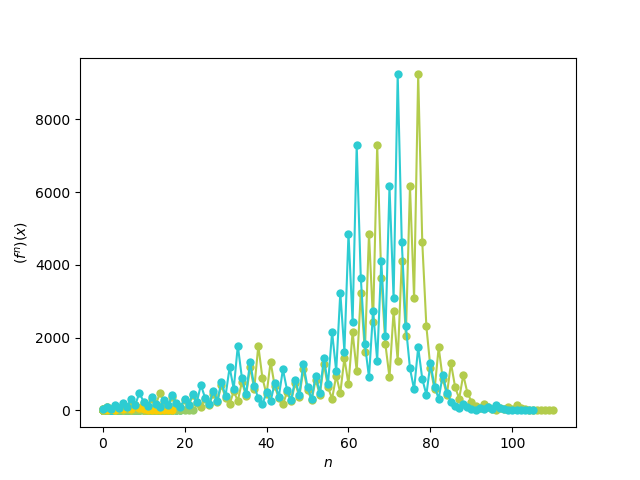
\includegraphics[width=8.3cm]{collatz.png}
  %\caption{\label{fig:collatz5}}
\end{figure}

\subsection{Numpy}

Рассмотрим пример цикла на питоне:
\begin{minted}{python}
  n = 10000
  a = []
  for i in range(n):
      a.append(sqrt(i / (n - 1))
\end{minted}
Что здесь может работать медленно?
\begin{enumerate}
    \item Цикл сам по себе работает не быстро из-за особенностей интерпретатора
        Python, и при простом содержимом цикла может быть гораздо затратнее
        содержимого.
    \item Вызов функции в питоне гораздо более затратен, чем в C++, частично
        из-за приведения типов и выбора из набора функций для разных типов.
        Рекурсии в питоне стоит также избегать.
\end{enumerate}

Варианты решения проблем: multiprocessing

JIT-компиляция. Pypy --- вместо интерпретатора питона,
делает байт-код, потом компилирует его с оптимозацией. Существенно (в разы)
ускорение, однако не поддерживает все библиотеки питона. Numba --- создаёт
скомпилированные версии функций, может быть применена только к части кода. Очень
новая, нет в репозиториях и т. п.

Другой вариант --- векторизация операций. Интерпретация кода происходит один
раз, например, в list comprehension.

Аналогичный подход --- в библиотеке numpy. Перепишем наш код:
\begin{minted}{python}
    import numpy as np
    n = 10000
    a = np.arange(n) # 0..(n-1)
    a = a * i / (n - 1)
    a = np.sqrt(a) # sqrt от каждого элемента.
\end{minted}
Всего 3 (а не 30000) вызова функции и решения о типе и т. д. Корень работает
быстро (используется ф-я на C, скорее всего). Подобная векторная идеология
интенсивно используется в языке R. Вообще, провалов производительности везде
можно избежать, и уменьшение скорости по сравнению с C++ может быть и не очень
большим (10 раз по сравнению с O3).

\begin{minted}{python}
    #numpy tutorial
    import numpy as np
    a = np.array([1, 2, 3, 4, 5, 6]) # array([[1,2],[3,4]])
    print(type(a)) # numpy.ndarray
    print(a.shape) # (6,)
    b = np.reshape(a, (2,3))
    # [[1,2,3],
    #  [4,5,6]]
    print(b[0,1]) # 2
    print(b.transpose())
    # create empty, with ones, random, zeros...
    np.empty((5, 4))
    ...zeros, ones...
    np.eye(3) # identity matrix
    np.random.random((2,2)) # uniform (linear distribution), [0, 1)
    np.random.random(5)
    # slices
    c = b[:,1:]
    print(c)
    # [[2, 3]
    #  [5, 6]]
    # bool indexing
    bi = (c%2 == 1)
    # [[False,  True],
    # [ True, False]], dtype=bool
    print(c[bi]) # [3, 5] # matrix as index,
                          # [i] ведут себя по-разному в зависимости от типа i
    c[c%2 == 1] # alternative
    c[c > 2] # [3, 5, 6]
    # data type
    x = np.array([1,2,3], dtype=np.float) # int, int64, float, float64...
    # math
    x = np.arange(100)
    x = 0.1 * x
    y = np.sin(x) + np.cos(x) # ...plot(x, y)
    y = x * y # поэлементно
    # matrix operations
    x = np.array([1,-1,2])
    y = np.array([3,5,7])
    np.dot(x,y) # 12, как скалярное произведение
    m = np.array([x1 * y1 for x1 in x for y1 in y])
    # [ 3,  5,  7, -3, -5, -7,  6, 10, 14], все со всеми
    m = np.reshape(m, (3, -1))
    # [[ 3,  5,  7],
    #  [-3, -5, -7],
    #  [ 6, 10, 14]]
    print(np.dot(m, x)) # [ 12, -12,  24]
    print(np.dot(x, m)) # [18, 30, 42]
\end{minted}


Рассмотрим
задачy: сгенерировать массив чисел наперёд заданной длины (!), числа псевдослучайные
с функцией распределения (вероятность найти число в интервале):
\begin{equation}
    f(x) = \frac{dw}{dx} \propto \exp(\sin(\pi x^2)),\; x \in (0, 1).
\end{equation}
и продемонстрировать корректность работы генератора.
\begin{enumerate}
  \item найти функцию распределания полученного генератора и сравнить с теорией
      на графике % 3 б
  \item найти и печатать на экран <<центр масс>> полученного
      распределения (среднее значение $x$), 0.561418%, 1 б
  \item для массива случайных точек из 10000 элементов измерить время генерации
      и нахождение среднего (суммарное), вывести на экран % 1 б за время, 1б за
      %хорошую скорость
\end{enumerate}

Решение. Числа будем генерировать, используя метод Монте-Карло на плоскости. Медленный метод:
\begin{minted}{python}
# -*- coding: utf-8 -*-

import time
import numpy as np

# число точек с нужным распределением
n = 200000

# функция распределения с максимумом, равным 1 при x \in (0, 1)
def f(x):
    return np.exp(np.sin(np.pi * x * x)) / np.e

def mean(x):
    return sum(x) / len(x)

rands = np.empty(n);

# slow generation
t0 = time.perf_counter()
i = 0
while i < n:
    r1 = np.random.rand()
    r2 = np.random.rand()
    if r2 < f(r1):
        rands[i] = r1
        i += 1

t1 = time.perf_counter()
print("slow generation took " + str(t1 - t0) + " s")
print("<x> = ", mean(rands)) # should be 0.561418
\end{minted}
На моём компьютере получается
\begin{minted}{bash}
    slow generation took 1.4595759409712628 s
    <x> =  0.561022241364
\end{minted}

Быстрый метод.
\begin{minted}{python}
# fast method of generation
t2 = time.perf_counter()
rands = np.array([])
m = n
while len(rands) < n:
    r1 = np.random.rand(m)
    r2 = np.random.rand(m)
    # list comprehension is fast, but to get huge speed-up we
    # also should compute f(r1) using vector operation
    r3 = f(r1)
    a = [x for ((x, y), z) in zip(zip(r1, r2), r3) if y < z]
    # ...but length(a) != n
    rands = np.append(rands, a)
    m = m - len(a) + 10000 # для простоты
rands = rands[:n] # обрезаем небольшой "хвост"
t3 = time.perf_counter()
print("fast generation took " + str(t3 - t2) + " s")
print("<x> = ", mean(rands))
\end{minted}
Получается:
\begin{minted}{bash}
    fast generation took 0.14974620402790606 s
    <x> =  0.561465849588
\end{minted}
Теперь нужно собрать числа по ведёркам.
\begin{minted}{python}
# распределяем по корзинкам (bins)
nb = 100
b = np.zeros(nb)
# медленный метод
t4 = time.perf_counter()
for x in rands:
    i = int(x * nb) # ok if x is always >=0 and < 1
    b[i] += 1
t5 = time.perf_counter()
print("slow buckets: " + str(t5 - t4) + " s")
# быстрый, "векторный" метод
t6 = time.perf_counter()
x = (rands * nb).astype(int) # element-wise to int
b = np.array([len(x[x==i]) for i in np.arange(nb)])
t7 = time.perf_counter()
print("fast buckets: " + str(t7 - t6) + " s")
# ещё один быстрый метод
t6 = time.perf_counter()
(b, bin_edges) = np.histogram(rands, nb, (0, 1))
t7 = time.perf_counter()
print("histogram: " + str(t7 - t6) + " s")
\end{minted}
Получилось:
\begin{minted}{bash}
    slow buckets: 0.26687249704264104 s
    fast buckets: 0.03806155297206715 s
    histogram:    0.004349093185737729 s
\end{minted}
Теперь построим ступеньками.
\begin{minted}{python}
# теперь построим
u = [[x, x] for x in b]
u = np.reshape(u, 2 * nb)
v = np.empty(2 * nb)
v[0] = bin_edges[0]
v[-1] = bin_edges[-1]
w = [[x, x] for x in bin_edges[1:-1]] # not includes the last
v[1:-1] = np.reshape(w, 2 * (nb - 1))
import matplotlib.pyplot as plt
plt.plot(v, u, "b-")
x = np.linspace(0, 1, 100)
plt.plot(x, f(x) * max(u), "r-")
plt.xlabel(r"$x$")
plt.ylabel(r"$f(x)$")
plt.show()
\end{minted}

%\begin{figure}
%  \centering
%  \includegraphics[width=8.3cm]{distribution_py.png}
%  \caption{Распределение сгенерированных чисел.}
%\end{figure}

\subsection{Matplotlib: настройки, gridspec}

\begin{minted}{python}
    import matplotlib
    import matplotlib.pyplot as plt
    from matplotlib import gridspec

    font = {"family" : "Liberation Serif",
            "weight" : "normal",
            "size"   : 10}
    matplotlib.rc("font", **font)
    matplotlib.rc("lines", linewidth=lw)
    matplotlib.rc("axes", linewidth=lw)

    plt.figure(figsize=(3.3,4.5),dpi=300) # in inches
    gs = gridspec.GridSpec(3, 2)
    gs.update(left=0.15, right=0.97, bottom=0.07, top=1.0, wspace = 0.55)
    plt.subplot( gs[0,:], aspect = T / 0.4 / 3 )
    plt.subplot( gs[1,:], aspect = T / 250 / 3 )
    plt.subplot( gs[2,1], aspect = 0.5 )
    plt.subplot( gs[2,0], aspect = a0[-1] - a0[0] )
    plt.savefig("qwe.pdf")
\end{minted}

\section{Что дальше?}

\subsection{Задача \# 5, множество Жулиа, 7 баллов}

Есть комплексное отображение:
\begin{equation}
    f(z) = z^2 - 0.4 + 0.6 i,
\end{equation}
И есть последовательность
\begin{equation}
    g(n) = f^n = f(f( ...)(z), \; n \text{ раз}.
\end{equation}
Задача: построить распределение $n: \; abs(g(n)(z)) <= 2$ в плоскости $z$ ($x \in
[-2,, 2]$, $y \in [-2, 2]$. Можно взять $400 \times 300$ точек, $150$ итераций.
\begin{enumerate}
\item 5 б. за график
\item 2 б. за палитру, красоту, подписи осей (tex), pdf, 12 см шириной.
\end{enumerate}

Замечания по задаче.
\begin{minted}{python}
z * z - 0.4 + 0.6j
plt.imshow(n - xys, origin = "lower", cmap = "cubehelix", interpolation = "none",
        extent = (x1, x2, y1, y2))
plt.clim(-n * 1 / 8, n)
plt.colorbar(label = r"$n$")
plt.xlabel(r"$\operatorname{Re} \, z$")
plt.ylabel(r"$\operatorname{Im} \, z$")
plt.tight_layout()
plt.savefig("julia.pdf")
\end{minted}

\subsection{FFI, scipy, ode, linalg...}

\subsection{Контрольная, 1 час, дома можно дорешать}

\newpage

\begin{enumerate}
    \item Составьте численную схему для решения уравнения
        \begin{equation}
            \frac{d^2 x}{dt^2} + \frac{dx}{dt} + x = 0.
        \end{equation}
    \item Дана группа --- множество чисел $\{1,2,..,p - 1\}$ с операцией умножения по модулю $p$,
        где $p$ --- простое число. Для $p = 7$ найдите (некоторые) подгруппы данной группы.
    \item Для интегрируемой функции $f$ найдите (с точностью до постоянного множителя) свёртку
        \begin{equation}
            g(x) = \int_{x - 1/2}^{x + 1/2} \int_{x_1 - 1/2}^{x_1 + 1/2} ... \int_{x_{n - 1} -
            1/2}^{x_{n - 1} + 1/2}
            f(x_n) \, dx_n \,
            ... \, dx_2 \, dx_1,
        \end{equation}
        где интегрирование производится $n$ раз, $n \gg 1$.
\end{enumerate}

\begin{enumerate}
    \item В равноудаленных точках численной сетки заданы числа $f_i$, $i \in \mathbb Z$.  На данной
        сетке можно ввести оператор трансляции, заменяющий числа $f_i$ на $f_{i - 1}$. Аналогичным
        образом оператор
        трансляции можно ввести для непрерывных функций. Найти генератор трансляции $\hat P$ для
        непрерывной функции $f(x)$, $x \in \mathbb R$ такой, что оператор трансляции на малое
        расстояние $a$ есть $\hat A f = f + a \hat P f$.
    \item Доказать, что если для любого элемента $a$ из некоторой группы выполнено условие $a \cdot
        a = e$, где $e$ --- единичный элемент, то для любых двух элементов группы $b$ и $c$
        выполнено равенство $bc = cb$. Приведите пример нетривиальной группы, для которой квадрат
        любого элемента равен единице.
    \item Для интегрируемой функции $f$ найдите (с точностью до постоянного множителя) свёртку
        \begin{multline}
            g(x) = \int_{-\infty}^\infty \int_{-\infty}^\infty ... \int_{-\infty}^\infty
            f(x_n) \exp\left[-(x_n - x_{n - 1})^2 \right] ...\\
            \exp\left[-(x_2 - x_1)^2 \right]
            \exp\left[-(x_1 - x)^2 \right]
            \, dx_n \, ... \, dx_2 \, dx_1,
        \end{multline}
        где интегрирование производится $n$ раз, $n \gg 1$.
\end{enumerate}

\begin{enumerate}
    \item Найти предел последовательности $a_i$ при $i \to \infty$, если $a_0 = 2$, а $a_{i + 1} =
        (a_i + 5 / a_i) / 2$.
    \item Дано множество чисел $\{1,2,..,p - 1\}$ с операцией умножения по модулю $p$.
        Для $p = 6$ найдите подмножества данного множества, образующие группы с данной групповой
        операцией.
    \item  Пусть $A$ и $B$ --- квадратные матрицы $n \times n$ ($n \gg 1$),
        коэффициенты которых --- независимые случайные числа с равномерным распределением на
        отрезке $[0, 1]$. Оцените среднее и дисперсию элементов матрицы --- произведения $A B$.
        Предложите метод для оценки среднего и дисперсии детерминанта матрицы $A$.
\end{enumerate}

\newpage

\section{Функциональное программирование. Why FP matters}

Функция высшего порядка --- функция, принимающая и (или) возвращающая другую функцию.

Зачем нужно оперировать функциями? Например, есть список
\begin{minted}{cpp}
    class mylist {
        mylist* next;
        double value;
    };
\end{minted}
Для double у нас есть много функций (sin, sqrt, арифметика, round, int). Хочется их всех применять
поэлементно для списка (можно реализовать шаблон с передачей функции или указателя на йункцию в
качестве аргумента).

Другой пример: пишем <<решатель>> уравнений движения частицы в произвольных электромагнитных полях.
Решатель принимает указатель на функцию двух аргументов ($\mathbf r$ и $t$), а поля удобно задавать
функциями со своими параметрами:
\begin{minted}{cpp}
    field plane_wave(vec r, double t, double a0, double phi)
    // ...
    field const_B(double a0)
    // ...
\end{minted}
Как их превратать в функцию двух аргументов? (частично применённые функции).

Зачем это может быть использовано?

Как и в структурном программировании, важна модульность. Небольшие простые модули проще пишутся,
легче отлаживаются (причём по отдельности). Модули общего назначения могут быть переиспользованы. 

Рассмотрим примеры.

(John Hughes, Why functional programming matters, 1990).

Haskell. Декларативный стиль, неизменяемые переменные, частичное применение функций, рекурсия
(оптимизация хвостовой рекурсии) вместо циклов, отложенные вычисления, вывод типов.

Решим задачу о генерации ровно $n$ псевдослучайных чисел со сложным распределением. Для этого
воспользуемся списками.

\begin{minted}{haskell}
-- список - либо пустой, либо сделанный конструктором
-- из элемента и "хвоста" (тоже списка)
data List a = Cons a (List a) | Nil
    deriving Show

-- алгебраические типы данных, в Rust - enum...
-- Как они могут быть устроены?
-- Др. пример: Option a = Sone a | None

-- определим сумму
sum Nil = 0
sum (Cons x xs) = x + sum_ xs

-- 0 и + определяют сумму; обобщим:
-- (...x + (y + (z + 0)))
-- 0 -> x, + -> f, скобки у функций не пишутся
foldr_ f x Nil = x
foldr_ f x (Cons y ys) = f y (foldr_ f x ys)
-- разобрать пример у доски?

-- sum -> foldr (+) 0
sum_ = foldr_ (+) 0
product = foldr_ (*) 1
-- anytrue, alltrue...

-- Можно заметить, что (foldr f x) заменяет в списке
-- все Cons на f а Nil на x.
-- Cons 3 (Cons 4 (Cons 5 Nil) -> (+) 3 ((+) 4 ((+) 5 0)) = 12

-- тогда (foldr Cons Nil) просто копирует список!

-- Склеим два списка
append a b = foldr_ Cons b a

-- Измерим длину списка
length_ as = foldr_ count 0 as
-- типы a и n совершенно разные!
count a n = n + 1

-- Ещё нам понадобатся функция, применяющая некоторую функцию _g_
-- к каждому элементу списка. Для этого Cons надо заменить на композицию
-- (cons . g), а Nil на Nil.
map_ f a = foldr_ (\x y -> Cons (f x) y) Nil a

-- Таким образом, из одной небольшой функции foldr получили
-- и map, и length, и sum и т. д.

-- Можно по-другому:
map__ _ Nil = Nil
map__ g (Cons x xs) = Cons (g x) (map__ g xs)
\end{minted}

Программы в функиональной парадигме --- функции из начального состояния в конечное. Композиция $f
\circ g, \; (f \circ g)(x) = f(g(x))$ --- композиция программ. Такая композиция может быть
организована через сохранение промежуточных результатов в файле. Однако файл может оказаться
слишком большим и, главное, условие окончания работы известно в программе f, а не в g, что мешает
композиции. Идея отложенных вычислений (lazy evaluation): функция g даёт результат по мере того,
как он требуется функции f. Могут ли отложенные вычисления ужиться с функциями с побочными
эффектами?

Примеры отложенных (ленивых) вычислений. Оперирование бесконечными списками. zeroes, fibs.
\begin{minted}{haskell}
tail (Cons x xs) = xs
zipWithPlus (Cons x xs) (Cons y ys) = Cons (f x y) (zipWithPlus xs ys)
fibs = Cons 0 (Cons 1 (zipWithPlus fibs (tail fibs)))
\end{minted}
Пример с отложенными матрицами, fusion.

\subsection{FP in C++ and Python}

\inputminted{cpp}{whyfpmatters.cpp}

Отложенные вычисления --- пример с пересечениями фигур.

map, reduce

\subsection{ООП в Erlang}

habr

\subsection{Maxwell, dispersion relation}

see Dropbox - prog (связанные осцилляторы)


\subsection{Theorem for free}

habr, аналитическое вычисление производных

constexpr?
shared ptr?
понятие о DSL

\bibliographystyle{unsrt}
\bibliography{lectures}

\end{document}
